\documentclass[twocolumn,tighten]{aastex62}

 \shortauthors{French $\&$ Wakker}
\usepackage{graphicx}
\usepackage{subfigure}
\usepackage{amsmath}

%\usepackage{dblfloatfix}    % To enable figures at the bottom of page

%\usepackage{dblfloatfix}
%\usepackage{stfloats}

%\usepackage{lipsum}

%\usepackage[breaklinks=true]{hyperref}
\usepackage{breakcites}
\usepackage{microtype}


\newcommand{\degrees}{\ensuremath{^{\circ}}}
\newcommand{\NII}{[\ion{N}{ii}]}
\newcommand{\SII}{[\ion{S}{ii}]}
\newcommand{\Halpha}{H\ensuremath{\alpha}}
\newcommand{\Hbeta}{H\ensuremath{\beta}}
\newcommand{\Lyalpha}{Ly\ensuremath{\alpha}}
\newcommand{\OonH}{\ensuremath{12+\log(\mathrm{O/H})}}

%\newcommand{\Lstar}{$L^{\**}$}
\newcommand{\Lstar}{$L^*$}
\newcommand{\kms}{$\rm km\, s^{-1}$}

\newcommand{\HI}{\mbox{H\,{\sc i}} }
\newcommand{\I}{\,{\sc i}}
\newcommand{\II}{\,{\sc ii}}
\newcommand{\III}{\,{\sc iii}}
\newcommand{\IV}{\,{\sc iv}}
\newcommand{\V}{\,{\sc v}}
\newcommand{\VI}{\,{\sc vi}}

\newcommand{\f}{\emph{f}/}


\graphicspath{{figures_final//}}

\begin{document}

%\title{Evidence for a Rotational Component in the CGM of Nearby Galaxies\footnote{Based on observations made with the Southern African Large Telescope (SALT).}}
\title{EVIDENCE FOR A ROTATIONAL COMPONENT IN THE CGM OF NEARBY GALAXIES\footnote{Based on observations made with the Southern African Large Telescope (SALT).}}


\author{David M. French}
\affil{Space Telescope Science Institute, 3700 San Martin Drive, Baltimore, MD 21218}
\affil{Department of Astronomy, University of Wisconsin, Madison, WI 53706, USA}

\author{Bart P. Wakker}
\affil{Department of Astronomy, University of Wisconsin, Madison, WI 53706, USA}


\cleardoublepage

\begin{abstract}

We present results of a study comparing the line-of-sight velocity of $\rm Ly\alpha$ absorbers relative to the rotation velocity of nearby galaxy disks in the local Universe ($z \leq 0.03$). We have obtained rotation curves via long-slit spectroscopy of 12 galaxies with the Southern African Large Telescope, and combine this dataset with an additional 17 galaxies with published rotation curves from the literature. Each galaxy appears within $3 R_{\rm vir}$ of a QSO sightline with available Cosmic Origin Spectrograph (COS) data covering the relevant $\rm Ly\alpha$ wavelength range. We present simple cylindrical and NFW galaxy halo rotation models to interpret these data in the context of probing three-dimensional galaxy halos via 1-dimensional QSO absorption-line spectroscopy. Relative to this model we find that up to $63\%$ of $\rm Ly\alpha$ absorbers have velocities consistent with co-rotation. Intriguingly, we find the $\rm Ly\alpha$ co-rotation fraction to decrease with galaxy luminosity (\Lstar) in a model independent fashion. Finally, we report that both anti-rotating absorbers and those found near luminous galaxies ($L \gtrsim 0.6$\Lstar) mostly have low Doppler $b$-parameters ($b \lesssim 50$ \kms). Absorbers consistent with co-rotation show a wide range of Doppler $b$-parameters. These results are broadly in agreement with the co-rotation fractions predicted by the \cite{stewart2011b} simulations, and furthermore provide some of the first observational evidence of the cold- and hot-mode accretion regimes predicted to occur in the low-z Universe. 

%provides some of the first observational evidence for cold-mode accretion onto sub-\Lstar~ galaxies in the low-$z$ Universe. 

%We discuss the implications of these results with respect to the theoretical predictions of cold versus hot mode accretion in the low-$z$ Universe.

\end{abstract}


\keywords{galaxies:intergalactic medium, galaxies:evolution, galaxies:halos, quasars: absorption lines}


\section{Introduction}
Our current Lambda Cold-Dark-Matter ($\Lambda$CDM) cosmology picture describes galaxies forming hierarchically out of overdensities in the underlying dark matter distribution. As the surrounding intergalactic medium (IGM) is funneled toward a growing galaxy, simulations predict the angular momentum of the inflowing gas is redistributed onto the disk and seeds the overall rotation of the galaxy (e.g., \citealt{stewart2011a, chen2003, sharma2005, brook2011, kimm2011, pichon2011, stewart2013}). As this infalling gas is responsible for birthing and continuing to feed the galaxies throughout their lifetimes, it is expected that the extended gaseous halos should rotate in the same sense as both the galactic disks and dark matter halos.  

In this $\Lambda$CDM picture, accretion falls broadly into two types. In the so-called ``hot-mode", gas shock-heats at the virial radius as it encounters the galaxy halo. The inner, more dense region of this hot gaseous halo then rains down onto the disk as it radiatively cools (e.g., \citealt{fillmore1984, bertschinger1985, danovich2012, shen2013}). However, most gas arrives cold ($T\sim 10^{4}$ K) from the IGM, and the proposed radiative shock is unstable to cooling. Thus this hot-halo scenario may not actually be created \citep{birnboim2003, keres2005, ocvirk2008, brooks2009, dekel2009}.


% From vandevoort2011 - Hence, hot accretion will dominate for the most massive haloes. The dominant form of accretion will thus depend on both the mass of the halo and accretion redshift 
%(Birnboim & Dekel 2003; Katz et al. 2003; Kere� et al. 2005; Ocvirk, Pichon & Teyssier 2008; Brooks et al. 2009; Kere� et al. 2009a; Crain et al. 2010)


%all this from Pichon 2011 (MNRAS 418, 2493?2507) See also Binney 1977. 

In contrast, as part of  the alternative ``cold-mode" accretion model, filaments of gas from the IGM would merge smoothly with the disk, thus converting a significant fraction of their infall velocity to rotational velocity of the galaxy \citep{keres2005, stewart2017}. The simulations of \cite{powell2011} agreed with these conjectures by showing that indeed, the accreting filaments connect rather smoothly to the disc, even in the presence of strong supernova driven winds. This cold-mode of accretion likely dominates the global growth of all but the most massive halos at high redshifts ($z \gtrsim 3$), and the growth of lower mass ($M_{\rm halo} \leq 5 \times 10^{11} ~M_{\rm *}$) objects at late times \citep{dekel2006, vandevoort2011}. Furthermore, cosmological SPH simulations such as those by \cite{stewart2011b, stewart2013} suggests that halo gas should co-rotate with disk-gas out to at least 100 kpc, and that absorption in intervening QSO sightlines should be able to accurately capture this rotation signature. 

%Galaxy rotation curves have been observed to extend at constant velocity out to... (cite...). It becomes increasingly difficult to measure gas rotation much farther from this however as the density rapidly decreases. Within this region the galaxy disks transition into circumgalactic medium (CGM), and eventually the CGM merges with the intergalactic medium (IGM). At what point, however, does the surrounding medium cease to circulate with the galaxy? A standard tool for probing gas at large radii from galaxies is QSO absorption line spectroscopy. 

\begin{deluxetable*}{l l l l l l l c l r}
%\rotate
\tablewidth{0pt}
\tabletypesize{\footnotesize}
\tablecaption{SALT Galaxy Observations\label{tab:params}}
\tablehead{
\colhead{Galaxy}	&  \colhead{R.A.}	&  \colhead{Dec.}  	&  \colhead{$v_{\rm sys}$}& \colhead{Published $v_{\rm sys}$} & \colhead{Type}	&  \colhead{$v_{\rm obs}$}	& \colhead{$v_{\rm rot} = v_{\rm obs} / \sin(\emph{i})$}	& \colhead{Obs. Date} & \colhead{$T_{\rm exp}$}  \\
			  	&          			&  			 	& \colhead{(\kms)}  				& \colhead{(\kms)}  		     	   &					&  \colhead{(\kms)}  		& \colhead{(\kms)}					&					& \colhead{(ks)} \\
\colhead{(1)}  	  	& \colhead{(2)}    	&  \colhead{(3)}   	& \colhead{(4)}  				& \colhead{(5)}    		     	   &	\colhead{(6)}  		& \colhead{(7)}    		&\colhead{(8)}  						& \colhead{(9)}  		& \colhead{(10)}   }
\startdata
 CGCG039-137 	& 11 21 27.0		& +03 26 41.7		& $6918 \pm24$				&	$6902 \pm 52^{a}$	& Scd			& $132 \pm 16$		& $143 \pm 25$			& 05 11 2016		& 700	\\ %done
 ESO343-G014	 	& 21 37 45.2		& $-$38 29 33.2	& $9139 \pm32$				&	$9162 \pm 45^{b}$	& S				& $203 \pm 32$		& $203 \pm 32$			& 05 16 2016		& 1000	\\ %done
 IC5325		 	& 23 28 43.4		& $-$41 20 00.5	& $1512 \pm8$					&	$1503 \pm 7^{c}$	& SAB(rs)bc		& \phantom{s}$53 \pm 5$	& $125 \pm 27$			& 05 17 2016		& 600	\\ %done
 MCG-03-58-009	& 22 53 40.9		& $-$17 28 44.0	& $9015 \pm19$				&	$9030 \pm 10^{d}$	& Sc				& $150 \pm 11$			& $171 \pm 22$			& 05 16 2016		& 1200	\\ %done
 NGC1566		& 04 20 00.4		& $-$54 56 16.1	& $1502 \pm15$				&	$1504 \pm 2^{e}$	& SAB(rs)bc		& \phantom{p}$64 \pm 8$	& $195 \pm 47$			& 10 18 2016		& 400	\\ %done
 NGC3513		& 11 03 46.1		& $-$23 14 43.8	& $1204 \pm12$				&	$1194 \pm 7^{c}$	& SB(s)c			& \phantom{s}$11 \pm 8$	& \phantom{s}$22 \pm 24$	& 05 26 2016		& 600	\\ %done
 NGC3633	 	& 11 20 26.2		& +03 35 08.2		& $2587 \pm7$					&	$2600 \pm 2^{f}$	& SAa			& $149 \pm 6$			& $157 \pm 9$				& 05 11 2016		& 1200	\\ %done
 NGC4536	 	& 12 34 27.1		& +02 11 17.3		& $1867 \pm33$				&	$1808 \pm 1^{g}$	& SAB(rc)bc		& $129 \pm 21$		& $148 \pm 39$			& 05 11 2016		& 1300	\\ %done
 NGC4939		& 13 04 14.4		& $-$10 20 22.6	& $3093 \pm33$				&	$3110 \pm 4^{e}$	& SA(s)bc			& $204 \pm 23$		& $234 \pm 39$			& 05 14 2016		& 500	\\ %done
 NGC5364	 	& 13 56 12.0		& +05 00 52.1		& $1238 \pm17$				&	$1241 \pm 4^{c}$	& SA(rs)bc pec		& $130 \pm 12$		& $155 \pm 23$			& 05 11 2016		& 700	\\ %done
 NGC5786	 	& 14 58 56.3		& $-$42 00 48.1	& $2975 \pm22$				&	$2998 \pm 5^{h}$	& SAB(s)bc		& $156 \pm 14$		& $172 \pm 25$			& 05 11 2016		& 250	\\ %done
 UGC09760	 	& 15 12 02.4		& +01 41 55.5		& $2094 \pm16$				&	$2023 \pm 2^{i}$	& Sd				& \phantom{s}$46 \pm 10$ & \phantom{s}$46 \pm 16$	& 05 11 2016		& 500	\\
 \hline
\enddata

\tablecomments{SALT targeted galaxies. Columns are as follows: 1) the galaxy name, 2), 3) R.A., Dec. in J2000, 4) measured galaxy systemic velocity, 5) published galaxy systemic velocity, 6) morphological type (RC3), 7) approaching side velocity, 8) receding side velocity, 9) observation date, and 10) exposure time. All observations used the RSS PG2300 grating.}
%\tablenotetext{a}{\cite{sdssDR3}} 
%\tablenotetext{b}{\cite{6dFDR3}}
%\tablenotetext{c}{\cite{RC3}}
%\tablenotetext{d}{\cite{mathewson1996}}
%\tablenotetext{e}{\cite{koribalski2004}}
%\tablenotetext{f}{\cite{RC3}}
%\tablenotetext{g}{\cite{lu1993}}
%\tablenotetext{h}{\cite{grogin1998}}
%\tablenotetext{i}{\cite{koribalski2004}}
%\tablenotetext{j}{\cite{RC3}}
%\tablenotetext{k}{\cite{dinella1996}}
%\tablenotetext{l}{\cite{giovanelli1997}}
%\tablerefs{\cite{giovanelli1997}}
\tablerefs{a. \cite{sdssDR3}; b. \cite{6dFDR3}; c. \cite{RC3}; d. \cite{mathewson1996}; e. \cite{koribalski2004}; f. \cite{lu1993}; g. \cite{grogin1998}; h. \cite{dinella1996}; i, \cite{giovanelli1997}}
 \label{salt_targets}
\end{deluxetable*}


Some observational evidence of cold-mode accretion has been obtained at higher redshifts. In pioneering studies focusing on the Mg\II~absorber kinematics and their connection with neighboring galaxies, \cite{charlton1998} and \cite{steidel2002} (and later \citealt{kacprzak2010, ho2017}) found tantalizing evidence that a significant fraction of Mg\II~absorbers have velocities that can be explained by an extended gaseous disk. Additionally, \cite{diamond-stanic2016} detect co-rotating H$\alpha$ emission and Mg\,{\sc ii} and Fe\,{\sc ii} absorption toward a Milky Way-like galaxy at $z=0.413$. However, as noted by \cite{steidel2002}, a simple extended disk model is insufficient to explain the observed bulk motion implied by their sample of 5 Mg\II~absorber-galaxy systems, and a rotating \emph{halo} may be a better model.


%However, as noted by Steidel 2002, a rotating \emph{halo} may be a better model than a simple extended thick disk model based on . 

Additionally, the picture may have changed since $z \sim 0.5$, the epoch 5 Gyr ago that most of these Mg\II~systems are probing. By $z \sim 0$ simulations (e.g., \citealt{keres2005, stewart2017}) predict a drop-off in cold-mode accretion and a decrease in the density of IGM filaments. Observational confirmation has been even more inconclusive in this low-redshift regime. In the largest such study, involving Ly$\rm \alpha$ absorber-galaxy kinematics, \cite{cote2005} probed the halos of nine galaxies using \emph{HST} observed background QSOs, and found that large warps would be needed to explain the velocity of \HI~absorbers by an extended rotating disk. Additionally, \cite{wakker2009} compiled a sample of 76 sightlines, which included only 4 galaxy-QSO systems for which the galaxy's rotation curve was known from the literature, and found only 1/4 of Ly$\alpha$ absorbers appeared to co-rotate with the associated galaxy disk. Similarly, \cite{kacprzak2011_kinematics} claim a reduction in Mg\II~co-rotation around $\rm \sim $\Lstar~ galaxies between $z\sim 0.5$ and $z\sim 0.1$. Approaching the question from a different angle, \cite{bowen2016} probed the halo of a single galaxy, NGC1097, with 4 nearby QSO sightlines, and suggests that an extended, slowly rotating disk with additional inflowing IGM material best matches observations. 


%The largest study of low-redshift, Ly$\rm \alpha$ absorber-galaxy kinematics was \cite{cote2005}, which worked with a  sample of 5 galaxy-absorber systems. 

%This cold-mode accretion should dominate the global growth of all galaxies at high redshifts (z ? 3) and the growth of low-mass (Mhalo ? 5 � 1011 M) objects at late times (Dekel & Birnboim 2006).

%his infalling gas is shock-heated and slowly cools (\cite{danovich2012}, \cite{shen2013}). As this infalling gas is responsible for birthing and continuing to feed the galaxies, it is expected that the extended gaseous halos should rotate in the same sense as both the galactic disks and dark matter halos. 

%As matter is funneled toward a growing galaxy, simulations predict conservation of angular momentum redistributes the angular momentum in this gas to match that of the halo and underlying dark matter as the gas is shock-heated and slowly cools (\cite{danovich2012}, \cite{shen2013}). As this infalling gas is responsible for birthing and continuing to feed the galaxies, it is expected that the extended gaseous halos should rotate in the same sense as both the galactic disks and dark matter halos. 

%There have been several studies with a sample size of one or a few aiming to compare the kinematics of the galaxy disk to absorption detected in it's CGM halo (e.g., C\^{o}t\'{e} et al. 2005; Wakker \& Savage 2009; Bowen et al. 2016; \textbf{MORE}). With these individual results we may be missing the forest for the sake of the individual trees. There has yet to be a more systematic search for observational evidence that the CGM is kinematically associated with galaxies in general.


%Numerous studies have shown a correlation between equivalent width and decreasing velocity difference between galaxies and IGM absorbers (e.g., \citealt{french2017}, MORE).

This current work aims to address many of these observational challenges. Firstly, by significantly increasing the sample size of galaxy-absorber systems, and secondly, by implementing a 3-dimensional rotating halo model to aid in the interpretation challenge inherent in a 1D sightline probing a 3D structure. To significantly improve observational statistics in this low-redshift regime, we have obtained rotation curves from the Southern African Large Telescope (SALT) for 12 nearby spiral galaxies which are located within $3 R_{\rm vir}$ of a background QSO observed by the Cosmic Origins Spectrograph (COS) on \textit{HST}. A literature search yielded an additional 17 galaxies with published rotation curves and known orientations. Each of these is probed by at least one QSO within $3 R_{\rm vir}$.

In Section \ref{data} we describe the selection and reduction of both SALT and COS spectra. In Section \ref{model} we present the rotating halo model we have developed to aid in the interpretation of our observations. In Section \ref{discussion} we discuss the overall results of this exercise and present a physically-motivated interpretation of these results. See Section \ref{summary} for a summary of our results and conclusions. Each galaxy-QSO system is discussed in detail in Appendix \ref{SALT_sample} (SALT-observed galaxies) and \ref{ancillary_data} (galaxies from the literature).




\begin{deluxetable*}{l l l l r r r}
\tablewidth{0pt}
\tabletypesize{\footnotesize}
\setlength{\tabcolsep}{0.15in}
\tablecolumns{7}
%\tablewidth{2.0pt}
\tablecaption{Summary of QSO Sample\label{tab:params}}
\tablehead{
\colhead{Target}  		&  \colhead{Galaxy} 			&  \colhead{R.A.}  		&  \colhead{Dec.}		& \colhead{z} 	&  \colhead{Program} &  \colhead{\tablenotemark{a} ${T_{\rm exp}}$}	\\
			  		&          					&  			 		& 		  			& 		     	&				  & \colhead{(ks)}}
\colnumbers
\startdata
1H0419-577  				&      NGC1566  		&      04 26 00.7  		&	$-$57 12 02.0  		&   0.10400  	& 11686		& 20429	\\
2E1530+1511				&	NGC5951			&	15 33 14.3		&	+15 01 03.0		&   0.09000	& 14071		& 9348	\\
3C232					&	NGC3067			&	09 58 20.9		&	+32 24 02.0		&   0.53060	& 8596		& 44662	\\
3C273.0  					&	NGC4536  		&      12 29 06.7  		&	+02 03 09.0 		&   0.15834  	& 12038		& 4002	\\
CSO295					&	NGC3432			&	10 52 05.6		&	+36 40 40.0		&   0.60900	& 14772		& 1088	\\
CSO1208					&	NGC3726			&	11 40 47.9			&	+46 22 05.0		&   0.11500	& 14729		& 3052	\\
FBQSJ0908+3246			&	NGC2770			&	09 08 38.8		&	+32 46 20.0		&   0.25989	& 14240		& 7430	\\
H1101-232  				&      NGC3513  		&      11 03 37.7  		&	$-$23 29 31.0  		&   0.18600  	& 12025		& 13341	\\
HE0429-5343  				&      NGC1566  		&      04 30 40.0  		&	$-$53 36 56.0 		&   0.04001  	& 12275		& 2067	\\
%HE0435-5304  			&      NGC1566  		&      04 36 50.9  		&      -52 58 47.0  		&   0.42616  	& 11520		& 8372	\\
%HE0439-5254  			&      NGC1566  		&      04 40 12.0  		&	-52 48 18.0  		&   1.05300  	& 11520		& 8402	\\
HE1228+0131  				&      NGC4536  		&      12 30 50.0  		&	+01 15 23.0  		&   0.11700  	& 11686		& 11036	\\
MRC2251-178  			&      MCG-03-58-009  	& 	22 54 05.9  		&	$-$17 34 55.0  		&   0.06609  	& 12029		& 5515	\\
MRK335					&	NGC7817			&	00 06 19.5		&	+20 12 11.0		&   0.02578	& 11524		&  5122	\\
MRK771					&	NGC4529			&	12 32 03.6		&	+20 09 30.0		&   0.06301	& 12569		& 1868	\\
MRK876					&	NGC6140			&	16 13 57.2		&	+65 43 11.0		&   0.12900	& 11524		& 12579	\\
%MS1047.3+3518			&	NGC3432			&	10 50 10.9		&	+35 02 02.0		&   0.04125	& 8316		&  8301	\\
PG0804+761				&	UGC04238		&	08 10 58.7		&	+76 02 43.0		&   0.10200	& 11686		& 5510	\\
PG1259+593				&	UGC08146		&	13 01 12.9		&	+59 02 07.0		&   0.47780	& 11541		&  9200	\\
PG1302-102  				&      NGC4939  		&      13 05 33.0  		&	$-$10 33 19.0  		&   0.27840  	& 12038		& 5979	\\
QSO1500-4140  			&      NGC5786  		&      15 03 34.0  		&	$-$41 52 23.0  		&   0.33500  	& 11659		& 9258	\\
%RBS567  				&      NGC1566  		&      04 39 38.7  		&	-53 11 31.0  		&   0.24300  	& 11520		& 8176	\\
RBS1503					&	NGC5907			&	15 29 07.5		&	+56 16 07.0		&   0.09900	& 12276		&  1964	\\
RBS1768  				&      ESO343-G014  	&   	21 38 49.9  		&	$-$38 28 40.0  		&   0.18299  	& 12936		& 6962	\\
RBS2000  				&      IC5325  			&      23 24 44.7  		&	$-$40 40 49.0  		&   0.17359  	& 13448		& 5046	\\
%RX\_J1002.9+3240		&	NGC3067			&	10 02 54.5		&	+32 40 39.0		&   0.83000	& 12603		&  7713	\\
RX\_J1017.5+4702			&      NGC3198			&	10 17 31.0		&	+47 02 25.0  		&   0.33544  	& 13314		& 8655     \\
RX\_J1054.2+3511			&	NGC3432			&	10 54 16.2		&	+35 11 24.0		&   0.20300	& 14772		&  533	\\
%RX\_J1117.6+5301			&	UGC06446		&	11 17 40.5			&	+53 01 51.0		&   0.15871	& 14240		&  4943	\\
RX\_J1117.6+5301  			&      NGC3631  		&      11 17 40.5  		&   	+53 01 51.0  		&   0.15871  	& 14240  		&  4943    \\
RX\_J1121.2+0326  			&      CGCG039-137, NGC3633  &   	11 21 14.0  	&	+03 25 47.0 		&   0.15200  	& 12248		& 2695	\\
%RX\_J1121.2+0326  		&      NGC3633  		&	11 21 14.0  		&	+03 25 47.0 		&   0.15200  	& 12248		& 2695	\\
RX\_J1142.7+4625			&	NGC3726			&	11 42 41.2			&	+46 24 36.0		&   0.11500	& 14772		&  2368	\\
RX\_J1236.0+2641			&	NGC4565			&	12 36 04.0		& 	+26 41 36.0		&   0.20920	& 12248		& 4235	\\
%SBS1116+523			&	UGC06399		&	11 19 47.9			&	+52 05 53.0		&   0.35568	& 14240		&  4949	\\
SBS1116+523				&	NGC3631			&	11 19 47.9			&	+52 05 53.0		&   0.35568	& 14240		&  4949	\\
SBS1503+570				&	NGC5907			&	15 04 55.6		&	+56 49 20.0		&   0.35894	& 12276		&  5163	\\
SDSSJ091052.80+333008.0	&	NGC2770			&	09 10 52.8		&	+33 30 08.0		&   0.11631	& 14240		&  7442	\\
SDSSJ091127.30+325337.0	&	NGC2770			&	09 11 27.3			&	+32 53 37.0		&   0.29038	& 14240		&  10028	\\
SDSSJ095914.80+320357.0	&	NGC3067			&	09 59 14.8		&	+32 03 57.0		&   0.56462	& 12603		&  2273	\\
%SDSSJ101622.60+470643.0	&	NGC3198			&	10 16 22.6		&	+47 06 43.0		&   0.82222	& 11598		& 4906  	\\
SDSSJ104335.90+115129.0	&	NGC3351			&	10 43 35.9		&	+11 05 29.0		&   0.79400	& 14071		& 4736	\\
%SDSSJ112005.00+041323.0  & 	NGC3633  		&      11 20 05.0  		&	+04 13 23.0 		&   0.54689  	& 12603		& 4708	\\
%SDSSJ112224.10+031802.0	&	NGC3633			&	11 22 24.1			&	+03 18 02.0		&   0.47528	& 12603		& 7588	\\
%SDSSJ112224.10+031802.0  & 	CGCG039-137 		&  	11 22 24.1  		&	+03 18 02.0 		&   0.47528  	& 12603		& 7588	\\
SDSSJ111443.70+525834.0  	& 	NGC3631  		&      11 14 43.7  		&   	+52 58 34.0  		&   0.07921  	& 14240  		& 13440   \\
SDSSJ112439.50+113117.0	&	NGC3666			&	11 24 39.4			&	+11 31 17.0		&   0.14300	& 14071		& 10427	\\
SDSSJ112448.30+531818.0	&	UGC06446, NGC3631	&	11 24 48.3		&	+53 18 19.0		&   0.53151	& 14240		& 7920	\\
%SDSSJ112632.90+120437.0	&	NGC3666			&	11 26 32.9			&	+12 04 37.0		&   0.97700	& 13314		& 8289	\\
%SDSSJ112756.70+115427.0	&	NGC3666			&	11 27 56.8			&	+11 54 27.0		&   0.50900	& 14145		& 5146	\\
SDSSJ135726.27+043541.4  	&	NGC5364  		&      13 57 26.3  		&	+04 35 41.0  		&   1.23453  	& 12264		& 14148	\\
SDSSJ151237.15+012846.0  	& 	UGC09760  		&      15 12 37.2  		&	+01 28 46.0  		&   0.26625  	& 12603		& 7590	\\
%SDSSJ152053.59+571122.1	&	NGC5907			&	15 20 53.7		&	+57 11 23.0		&   0.02952	& 13654		&  3753	\\
TON1009					&	NGC2770			&	09 09 06.2		&	+32 36 30.0		&   0.81028	& 12603		&  4740	\\
TON1015					&	NGC2770			&	09 10 37.0		&	+33 29 24.0		&   0.35400	& 14240		&  4774	\\
\hline
\enddata
%\tablenotetext{a}{Total exposure time and S/N ratio is given for multi-orbit exposures.}
\tablecomments{
\tablenotetext{a}{$T_{\rm exp}$ gives the total G130M integration time if multiple exposures were taken.}}
\end{deluxetable*}


\section{Data and Analysis} \label{data}

\subsection{SALT Data}
Our sample contains 12 galaxies observed with the Southern African Large Telescope (SALT) Robert Stobie Spectrograph (RSS) in longslit mode \citep{burgh2003, kobulnicky2003, buckley2006, odonoghue2006}. These 12 were selected from a larger pool of 48 submitted targets by the SALT observing queue. We chose these 48 possible targets for their proximity to background QSOs whose spectra contained promising Ly$\alpha$ lines. Finally, we only included galaxies with $z \leq 0.33$ ($cz \leq 10,000$ \kms), angular sizes less than 6' to enable easy sky subtraction using the outer edges of the slit and thus avoiding additional, off-target exposures, and surface brightnesses sufficient to keep exposure times below $\sim 1300 s$. Table \ref{salt_targets} summarizes these observations. Data were taken for 2 additional galaxies, NGC3640 and NGC2962, but proved unusable due to issues with spectral identification and low signal-to-noise (respectively).

%All SALT galaxy spectra were reduced and extracted using the standard PySALT reduction package (\textbf{\begin{table*}[ht]\footnotesize. 


All SALT galaxy spectra were reduced and extracted using the standard PySALT reduction package \citep{crawford2010}\footnote{http://pysalt.salt.ac.za/}, which includes procedures to prepare the data, correct for gain, cross-talk, bias, and overscan, and finally mosaic the images from the 3 CCDs. Next, we rectify the images with wavelength solutions found via Ne and Ar arc lamp spectra line identification. Finally, we perform a basic sky subtraction using an off-target portion of the spectrum, and extract 5-10 pixel wide 1-D strips from the reduced 2-D spectrum. 

For each resulting 1-D spectrum, we identify the H$\alpha$ emission lines and perform a non-linear least-squares Voigt profile fit using the Python package LMFIT\footnote{\url{http://cars9.uchicago.edu/software/python/lmfit/contents.html}}. While normally Gaussian profiles are used for fitting emission lines, we found a Voigt profile resulted in a better fit of the peak velocity (which is the measurement of prime importance for this analysis). The line centroid and 1$\sigma$ standard errors are returned, and these fits are then shifted to rest-velocity based on the galaxy systemic redshift with heliocentric velocity corrections calculated via the IRAF \emph{rvcorrect} procedure. The final rotation velocity is calculated by then applying the inclination correction, $v_{\rm rot} = v / \sin(i)$. 

Final errors are calculated as a quadrature sum of $1\sigma$ fit errors, systemic redshift error, and inclination uncertainty as follows:


%\begin{equation}
%\begin{split}
%	\sigma^2 = \left( \frac{\partial v_{rot}}{\partial \lambda_{obs}} \right)^2 (\Delta \lambda_{obs})^2 + \left(\frac{\partial v_{rot}}{\partial v_{sys}} \right)^2 (\Delta v_{sys})^2 + \\
%	\left( \frac{\partial v_{rot}}{\partial i} \right)^2 (\Delta i)^2,
%\end{split}
%\end{equation}

\begin{eqnarray} \label{error_calculation}
	\nonumber
	\sigma^2 = \left( \frac{\partial v_{rot}}{\partial \lambda_{obs}} \right)^2 (\Delta \lambda_{obs})^2 + \\
	\nonumber
	\left(\frac{\partial v_{rot}}{\partial v_{sys}} \right)^2 (\Delta v_{sys})^2 + \\
	\left( \frac{\partial v_{rot}}{\partial i} \right)^2 (\Delta i)^2,
\end{eqnarray}


\noindent where $\Delta \lambda_{obs}$, $\Delta v_{sys}$, and $\Delta i$ are the errors in observed line center, galaxy redshift, and inclination, respectively. We determine the inclination error by calculating the standard deviation of the set of all axis ratio values available in NED for each galaxy. This inclination component tends to dominate the error for low-inclination galaxies.

The final physical scale is calculated using the SALT image scale of 0.1267 arcsec/pixel, multiplied by the 4-pixel spatial binning, and converted to physical units using a redshift-independent distance if available, and a Hubble flow estimate if not. We adopt a Hubble constant of $H_0= 71$ \kms~$\rm Mpc^{-1}$ throughout.

Finally, we calculate our approaching and receding velocities via a weighted mean of the outer 1/2 of each rotation curve, with errors calculated as weighted standard errors in the mean. Our final redshifts are calculated by forcing symmetric rotation, such that the outer 1/2 average velocity for each side matches in magnitude. The upper-left panel of Figure \ref{model_fits} shows an example of this; the black points and error bars are the observed rotation measurements, the dark green lines show the average rotation velocity for the outer 1/2 edge of each rotation curve, and the green shading shows the $1\sigma$ error for this average value. See Appendix \ref{SALT_sample} for rotation curves and finder charts for each observed galaxy. 



\subsection{Additional Galaxy Data}
We have augmented our observed sample of galaxies with an additional 17 systems from the literature. While rotation curves for many galaxies have been published, a far smaller sample also included the necessary orientation information for our purposes. Of these, only the 17 included here were also relatively isolated and within $3 R_{\rm vir}$ of a background QSO with sufficient spectral coverage and signal-to-noise. The resulting sample come from a variety of sources, and we have endeavored to keep the galaxy properties (e.g., \emph{i}, $v_{\rm sys}$) adopted by the original data authors. For a small subset of these we have adopted more modern inclination and/or position angle measurements where appropriate (see Appendix \ref{ancillary_data} for details). We used the plot digitization software WebPlotDigitizer\footnote{WebPlotDigitizer; http://arohatgi.info/WebPlotDigitizer} to extract rotation curve data from figures when necessary. Rotation velocity errors are calculated with Eq. \ref{error_calculation} as for the SALT observed sample.




\begin{figure*}[ht!]
        \centering
        \vspace{0pt}
%        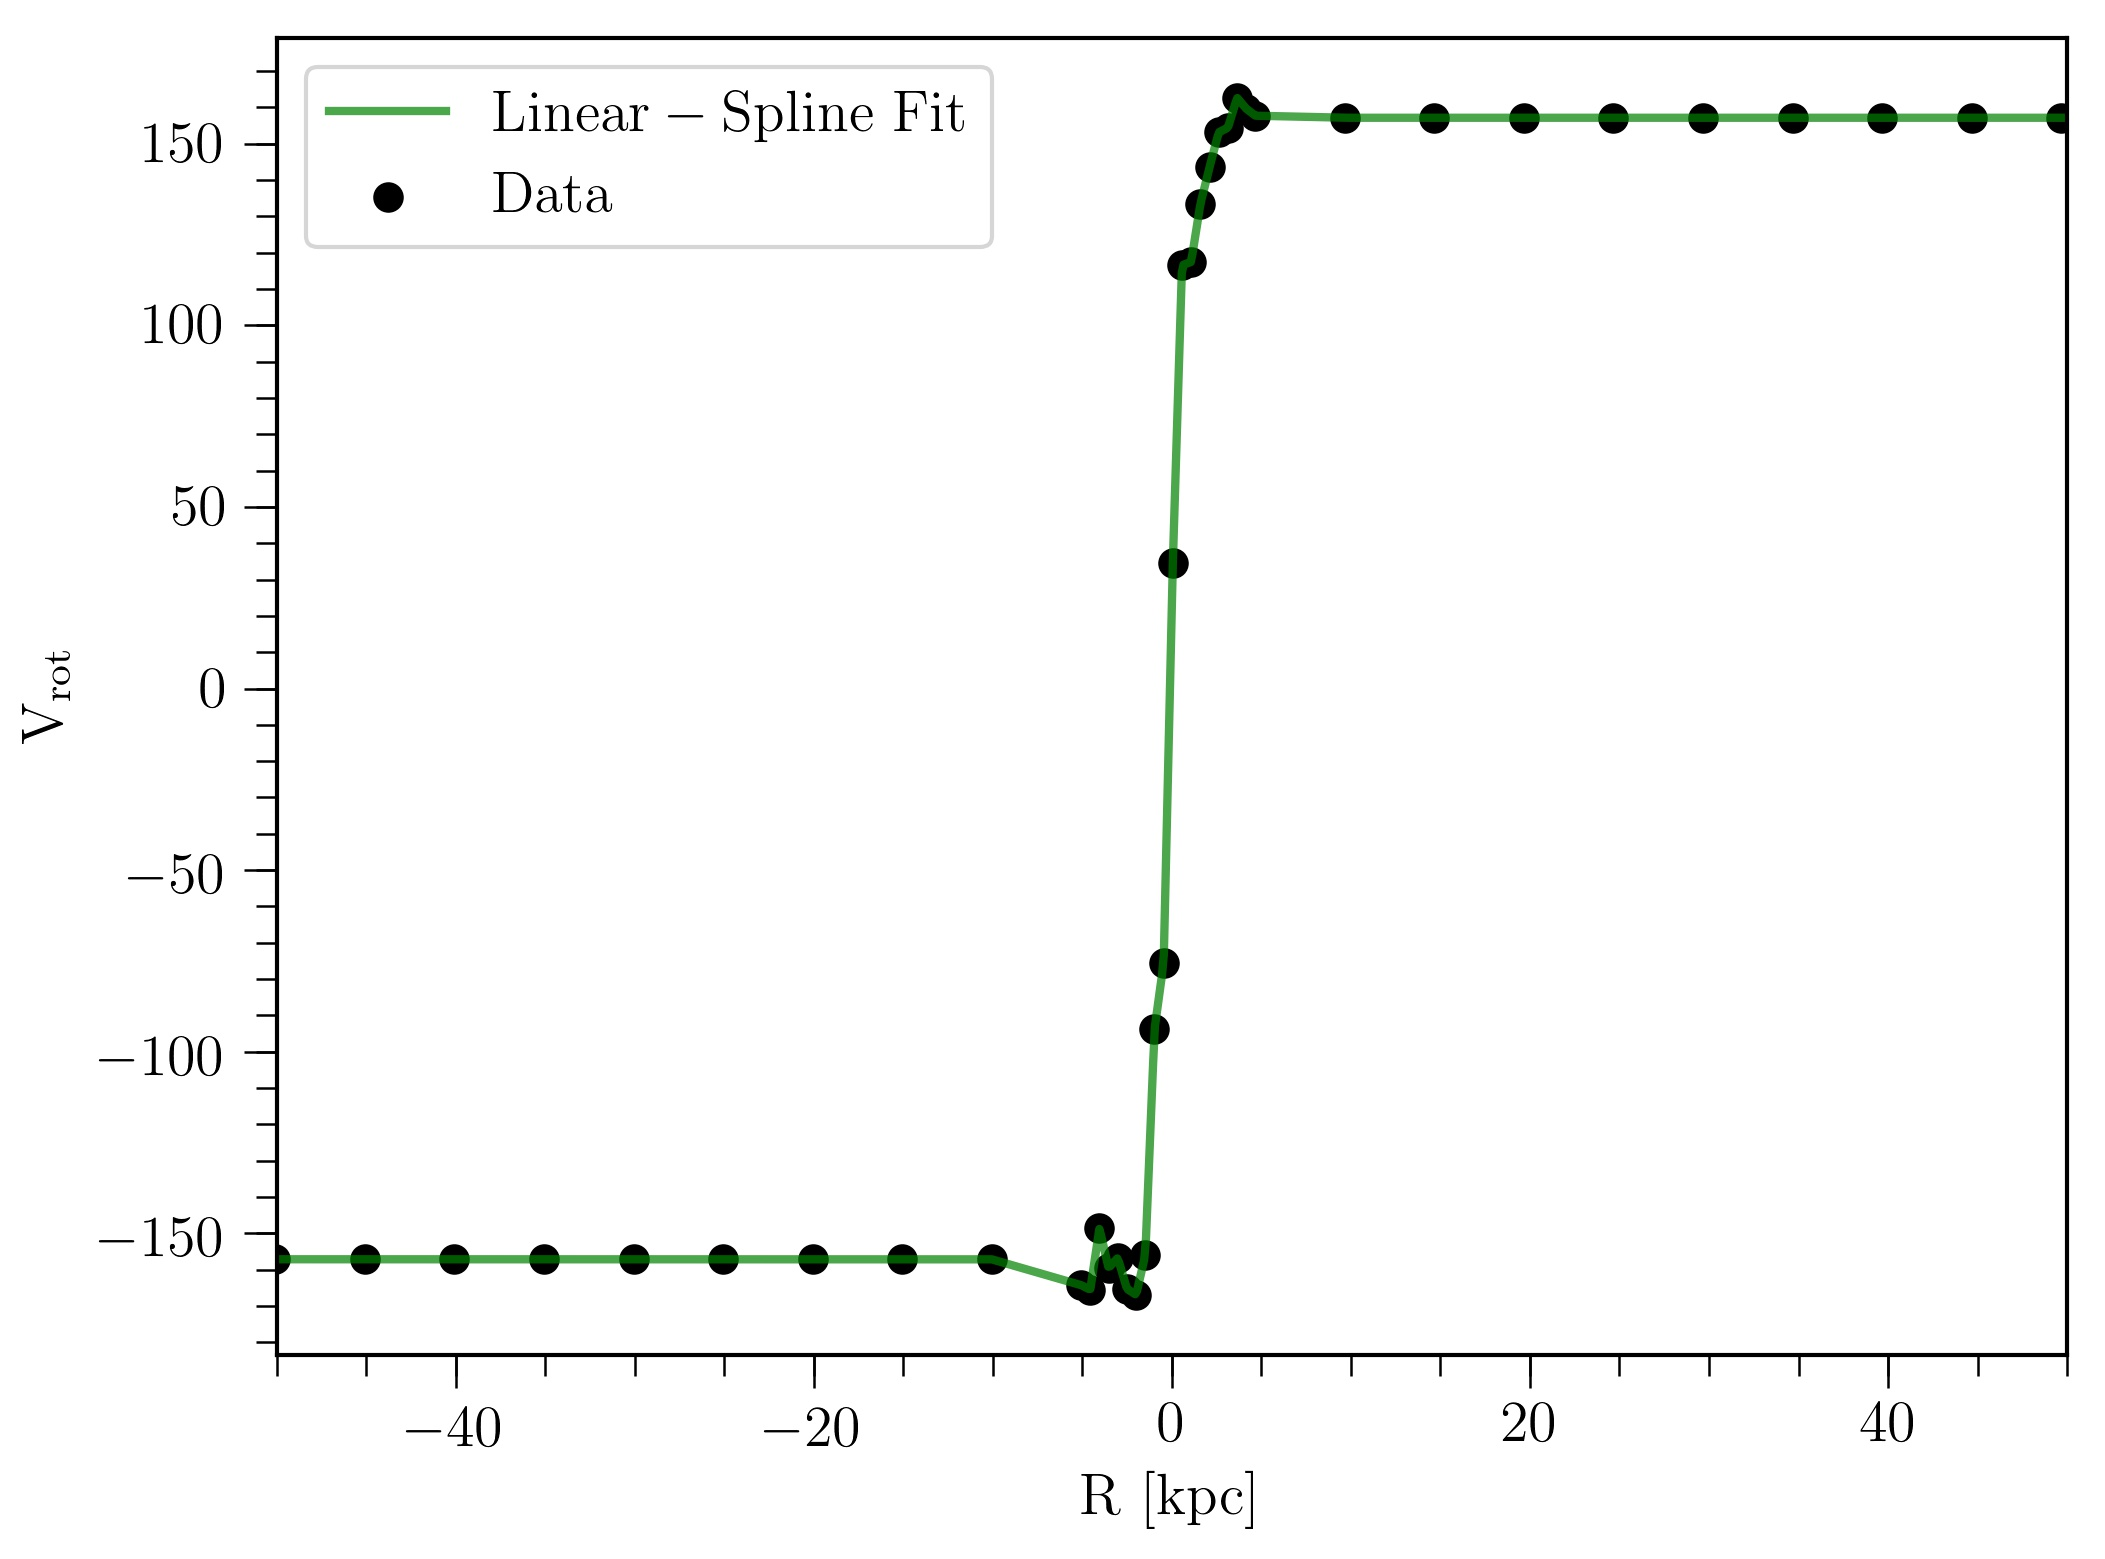
\includegraphics[width=0.36\textwidth]{NGC3633_splineFit_linear.jpg}
        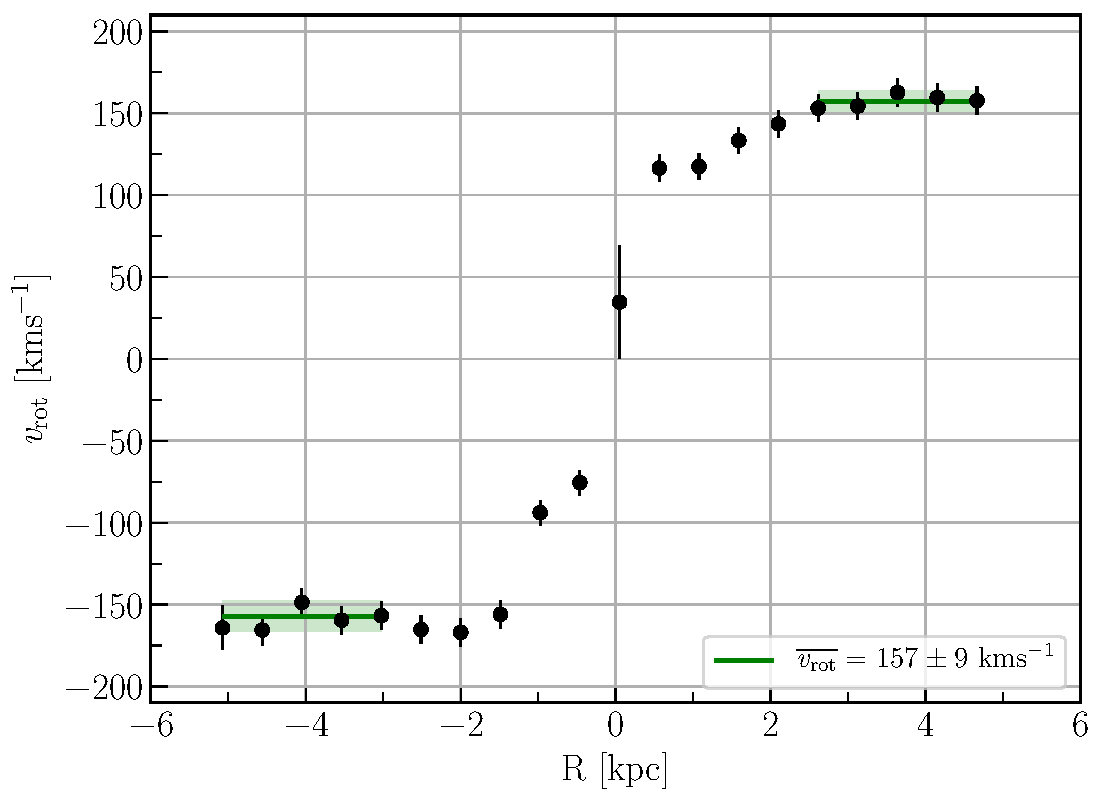
\includegraphics[width=0.33\linewidth]{NGC3633-rotation_curve_nice3.pdf}
%        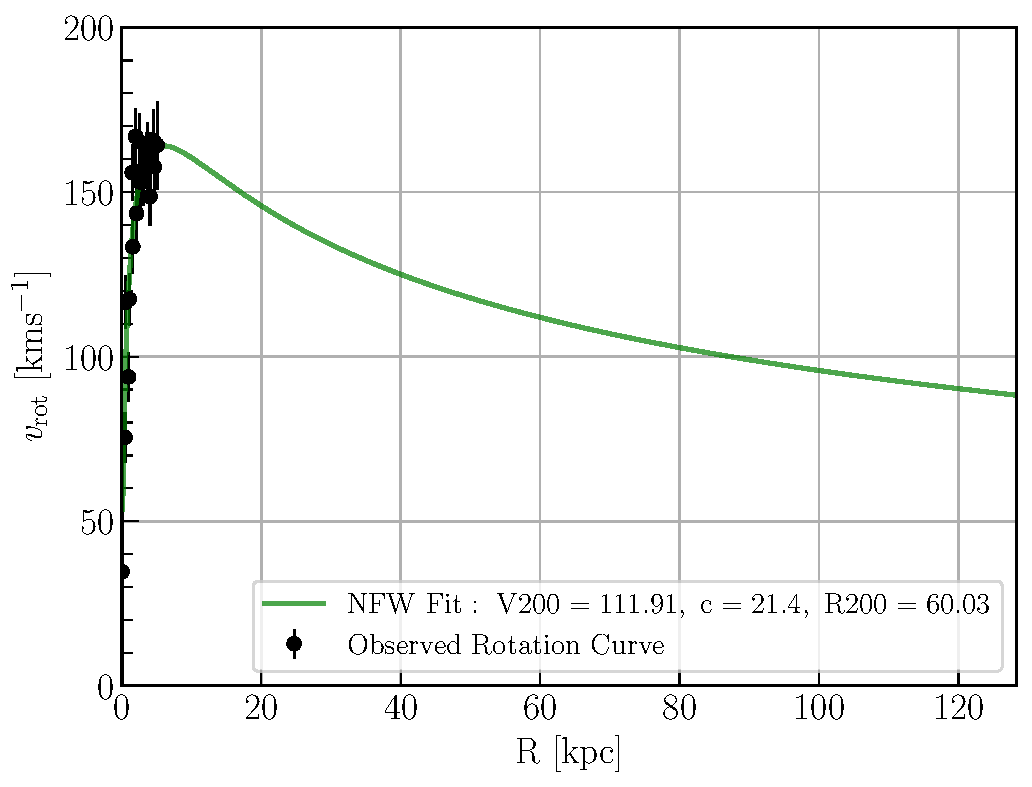
\includegraphics[width=0.319\linewidth]{NGC3633-NFW_fit_Rvir.pdf}
        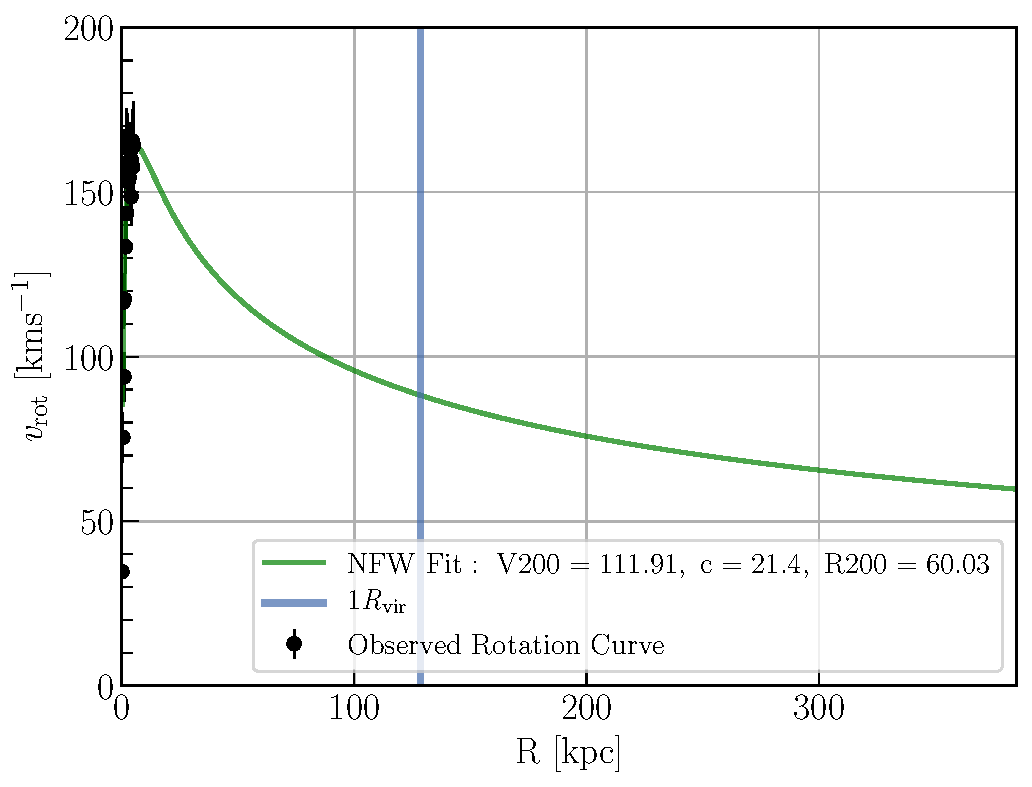
\includegraphics[width=0.319\linewidth]{NGC3633-NFW_fit_Rvir_times3_2.pdf}
        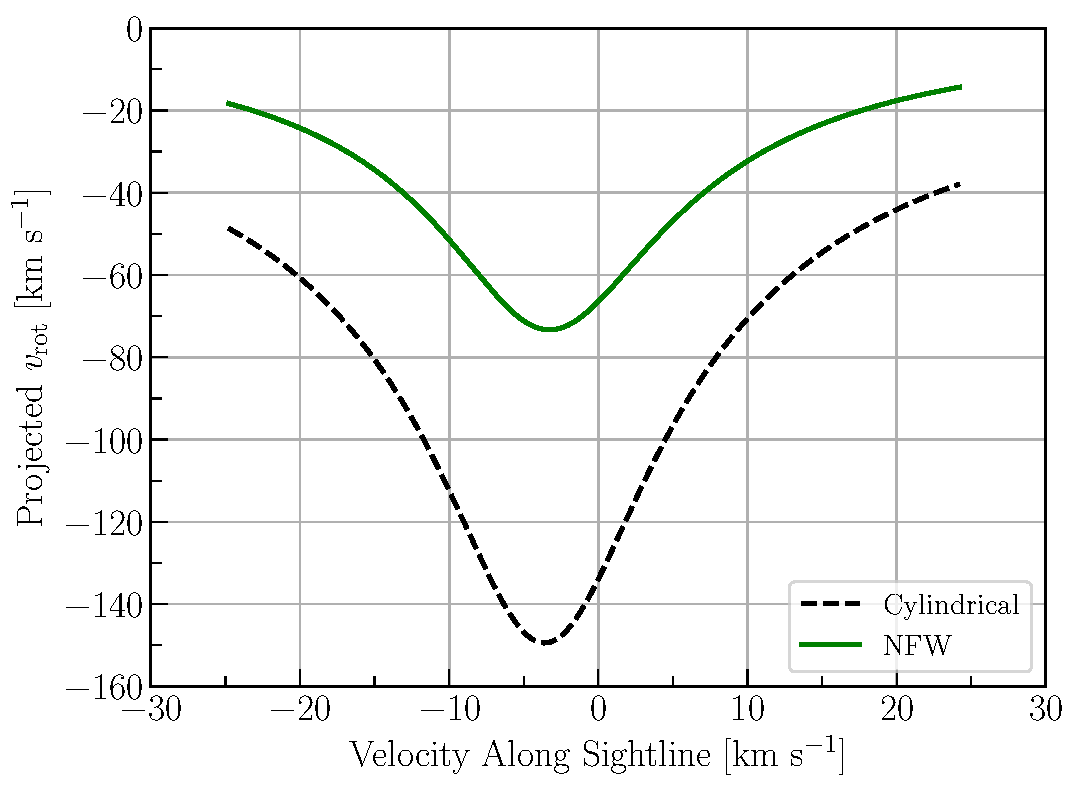
\includegraphics[width=0.331\linewidth]{NGC3633-RX_J1121_2+0326_model_plot4.pdf}
        
	\vspace{20pt}
	
        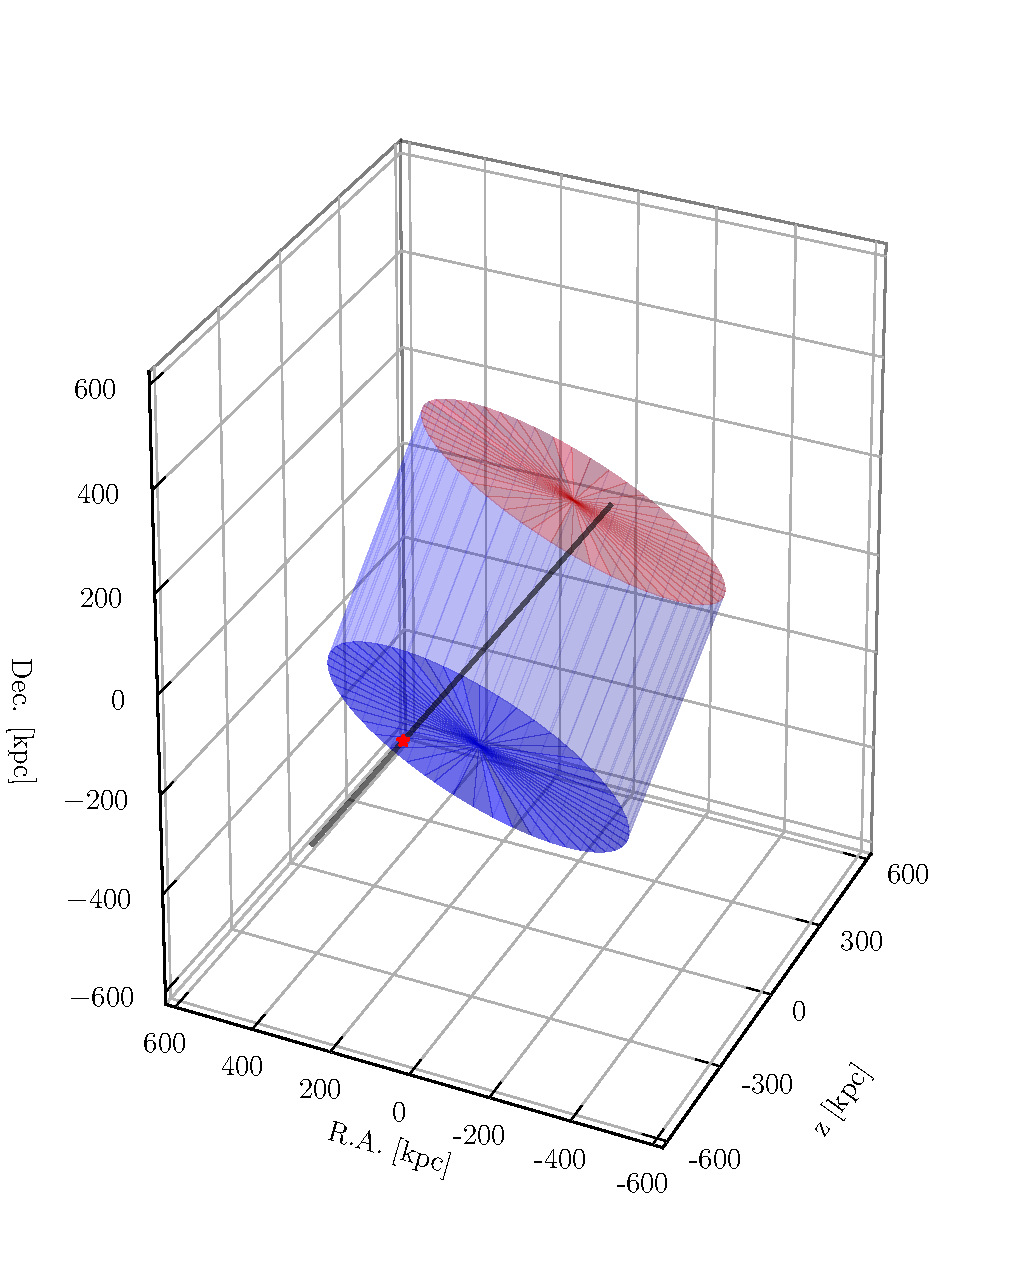
\includegraphics[width=0.32\linewidth]{NGC3633-RX_J1121_2+0326_3Dmodel_plot1_2.pdf}
        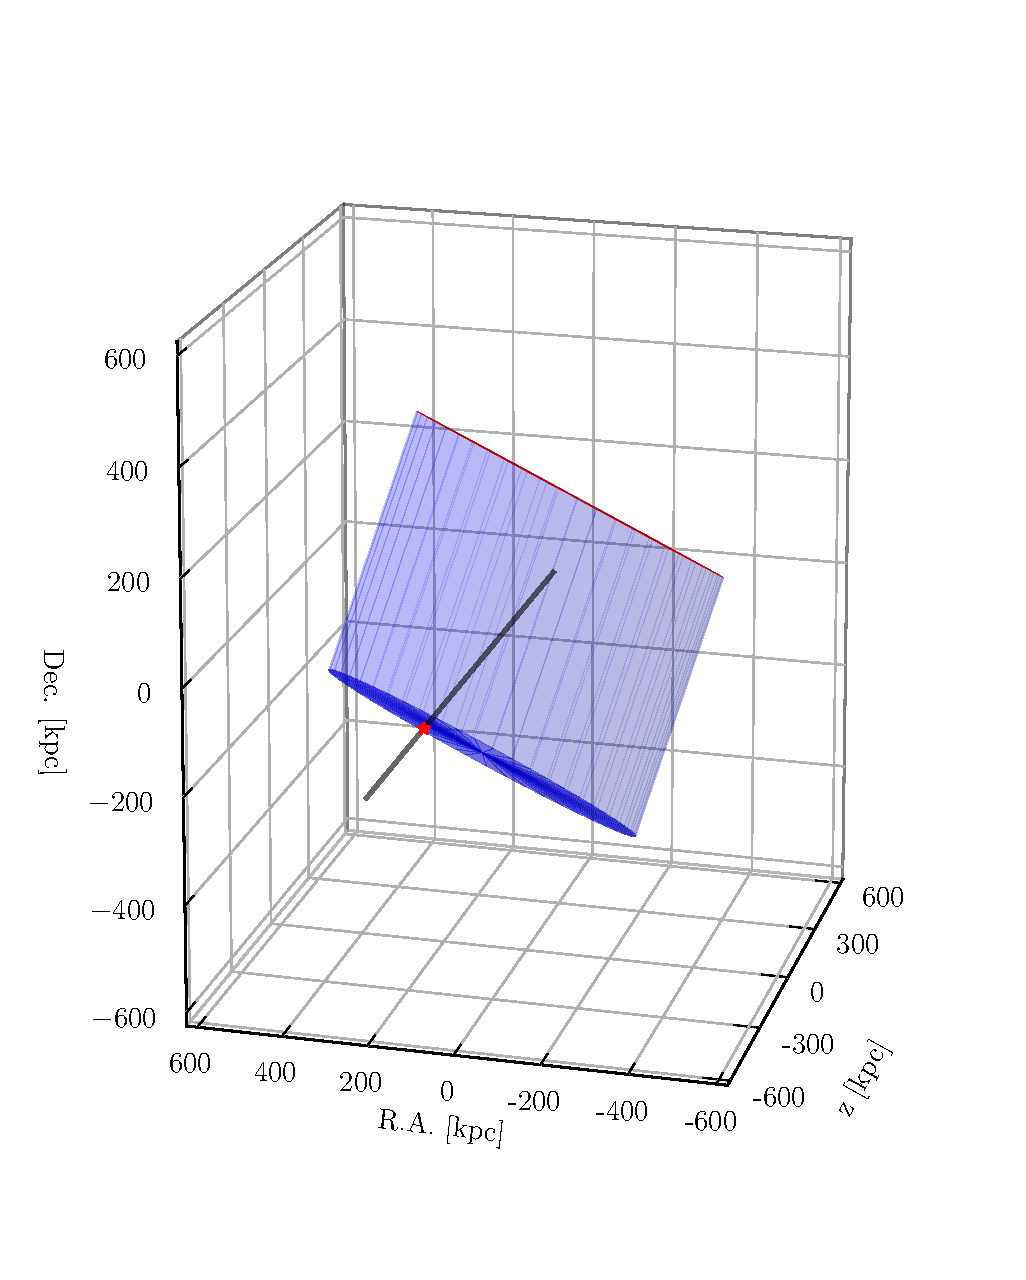
\includegraphics[width=0.32\linewidth]{NGC3633-RX_J1121_2+0326_3Dmodel_plot2_2.pdf}
        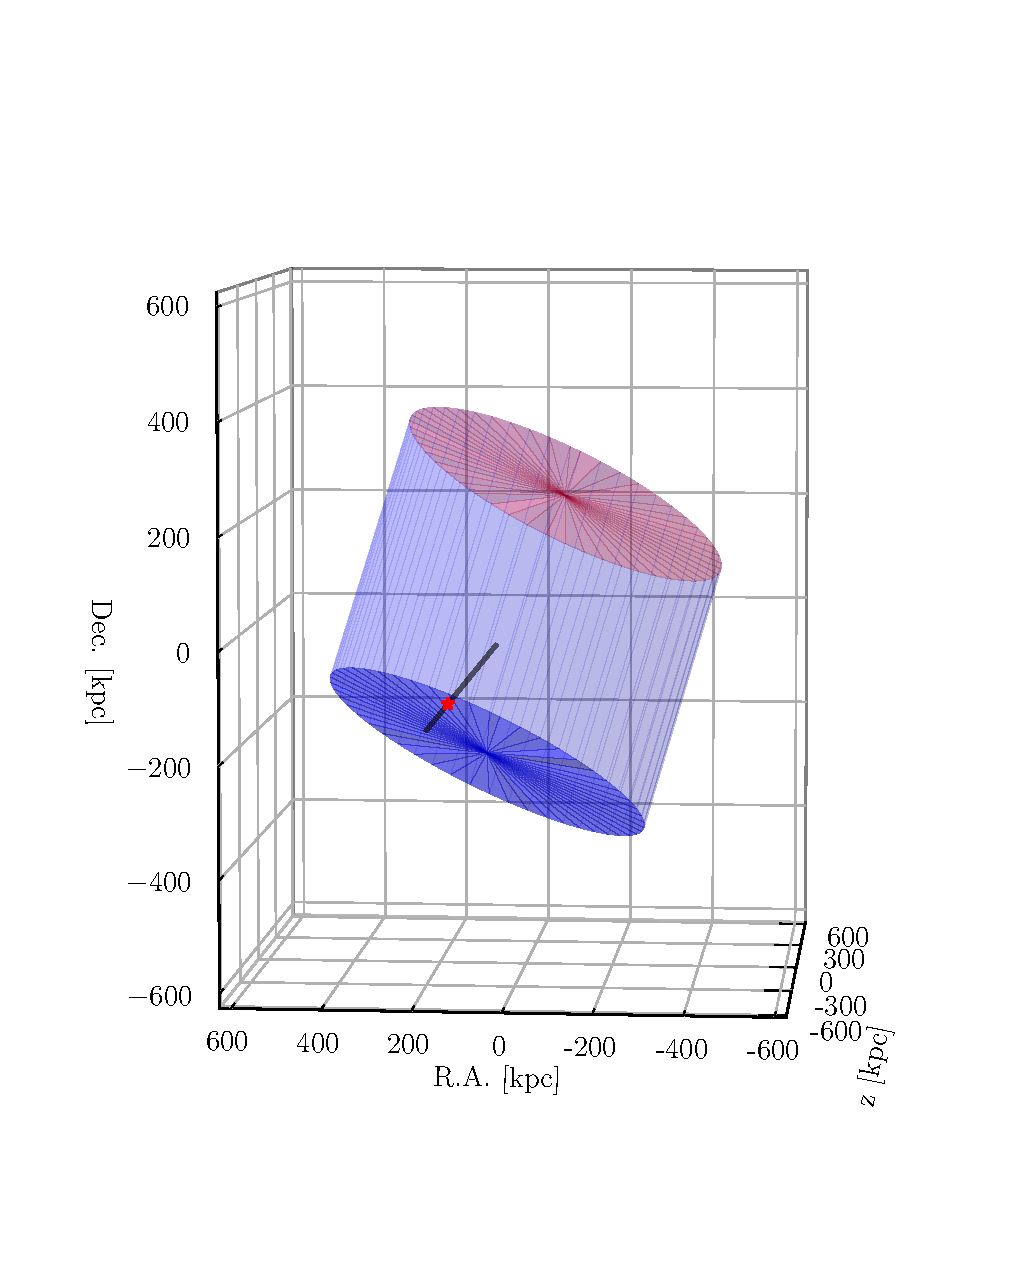
\includegraphics[width=0.32\linewidth]{NGC3633-RX_J1121_2+0326_3Dmodel_plot3_2.pdf}
        \caption{\small{\textbf{Top:} Left: The rotation curve for NGC3633 is shown in black, with the outer 1/2 mean rotation velocity indicated in green. Our cylindrical model simply extends this green average velocity out to $3 R_{\rm vir}$.  Middle: The observed rotation curve is again shown in black, with an NFW profile fit overlaid in green extending to $3 R_{\rm vir}$ ($1 R_{\rm vir}$ is shown by the vertical blue line).  Right: The resulting model velocity predictions for the cylindrical and NFW models are shown in dashed-black and solid-green (respectively). \textbf{Bottom:} A 3D example mockup of our halo rotation model showing the orientation and extent of the NGC3633 model from 3 different viewing angles. The approaching extreme edge of the NGC3633 cylindrical halo is shown by dark-blue oval, with the far edge shown in red. The black line shows the location of the sightline toward RX\_J1121.2+0326 as it penetrates the halo, with a red star marking the first intercept point.}}
%        \vspace{-5pt}
%        \label{3D_model}
	\label{model_fits}
        \vspace{10pt}
\end{figure*}



\subsection{COS Spectra}
The Barbara A. Mikulski Archive for Space Telescopes (MAST) archives yield 19 QSO targets observed by COS which lie within $3 R_{\rm vir}$ of our SALT galaxies. These targets vary widely in signal-to-noise from approximately 5 to 100 due to our choosing them based only on their proximity to galaxies with known rotation. The reduction procedure for these spectra follow those described by \cite{wakker2015} and \cite{french2017}. In short, spectra are processed with CALCOS v3.0 or higher and are aligned using a cross-correlation, and then shifted to make sure that (a) the velocities of the interstellar lines match the 21-cm HI profile, and (b) the velocities of lines in a single absorption system line up properly. Multiple exposures are combined by summing total counts per pixel before converting to flux. The COS instrument is described in detail by \cite{green2012}.

Once reduced we make a fourth-order or lower polynomial continuum fit in the region around each absorption line (typically within a 4000 \kms~window around each line) and measure integrated equivalent widths. To recover accurate Doppler $b$-parameter measurements, we then fit a Voigt profile to each line using the VoigtFit package by \cite{krogager2018}. The VoigtFit routine takes into account instrumental broadening by assuming a Gaussian with FWHM equal to the instrument spectral resolution (typically 17 \kms~for these COS spectra).

%combined via the method of \cite{wakker2015}, which helps corrects the COS wavelength scale misalignments produced by CALCOS. 


%\begin{figure*}[h]
%        \centering
%        \vspace{0pt}
%%        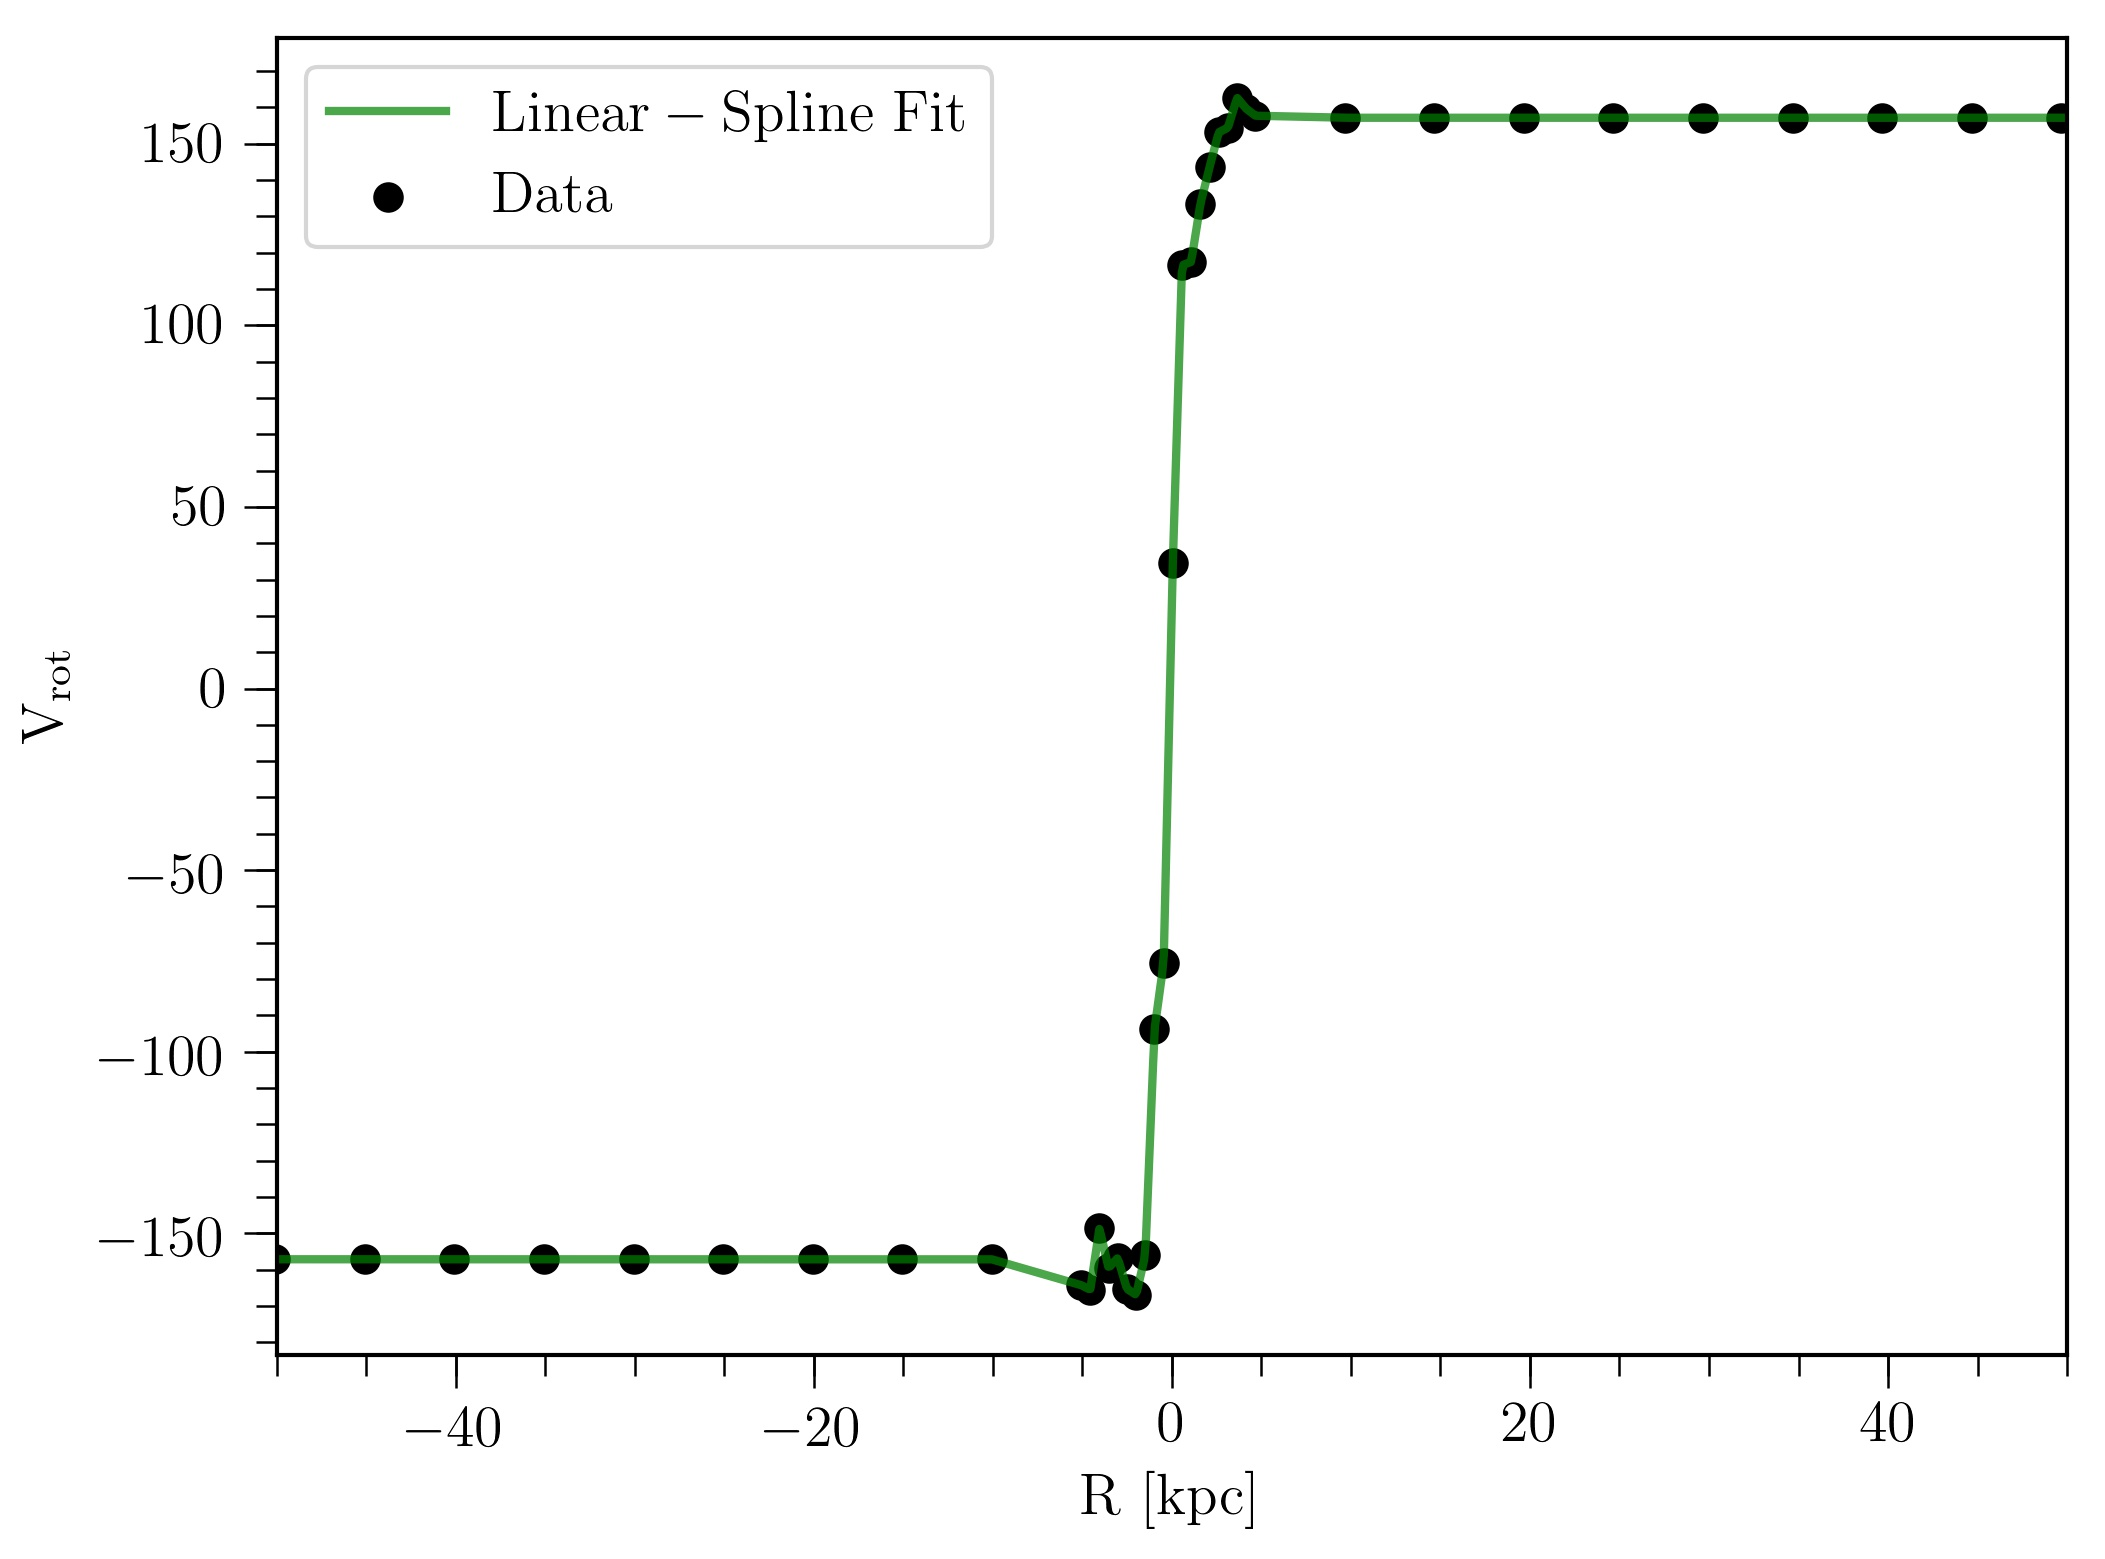
\includegraphics[width=0.36\textwidth]{NGC3633_splineFit_linear.jpg}
%        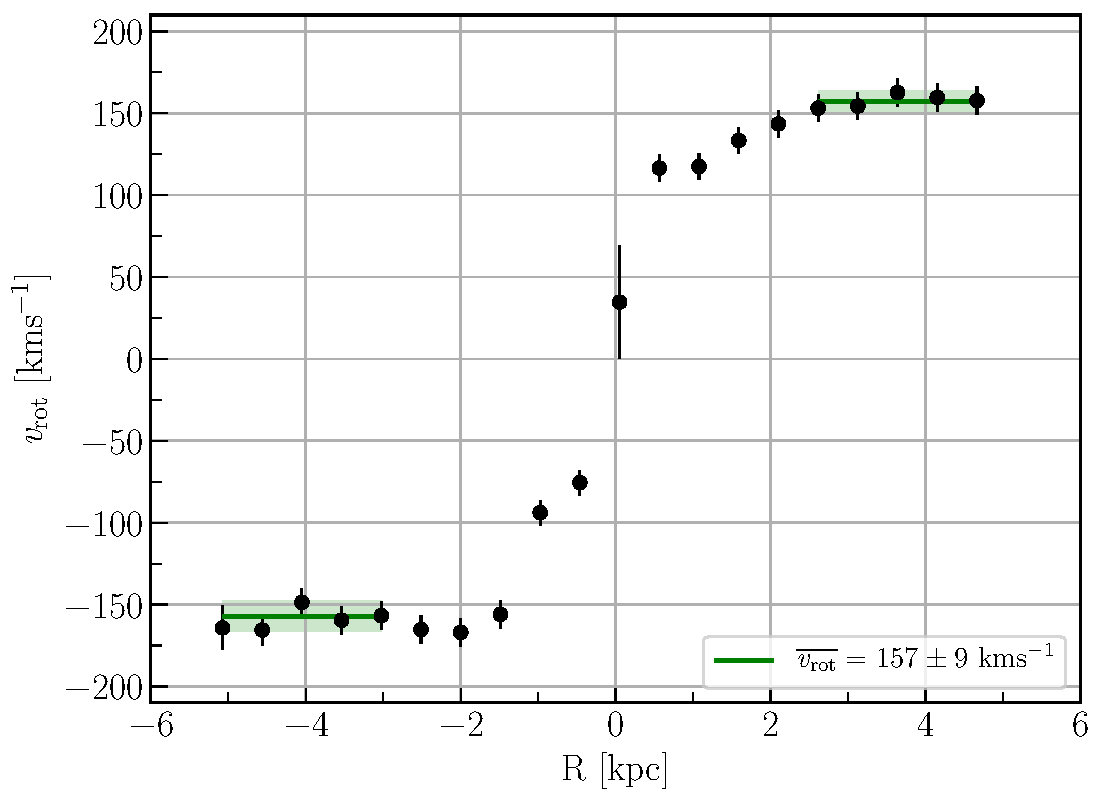
\includegraphics[width=0.33\linewidth]{NGC3633-rotation_curve_nice3.pdf}
%%        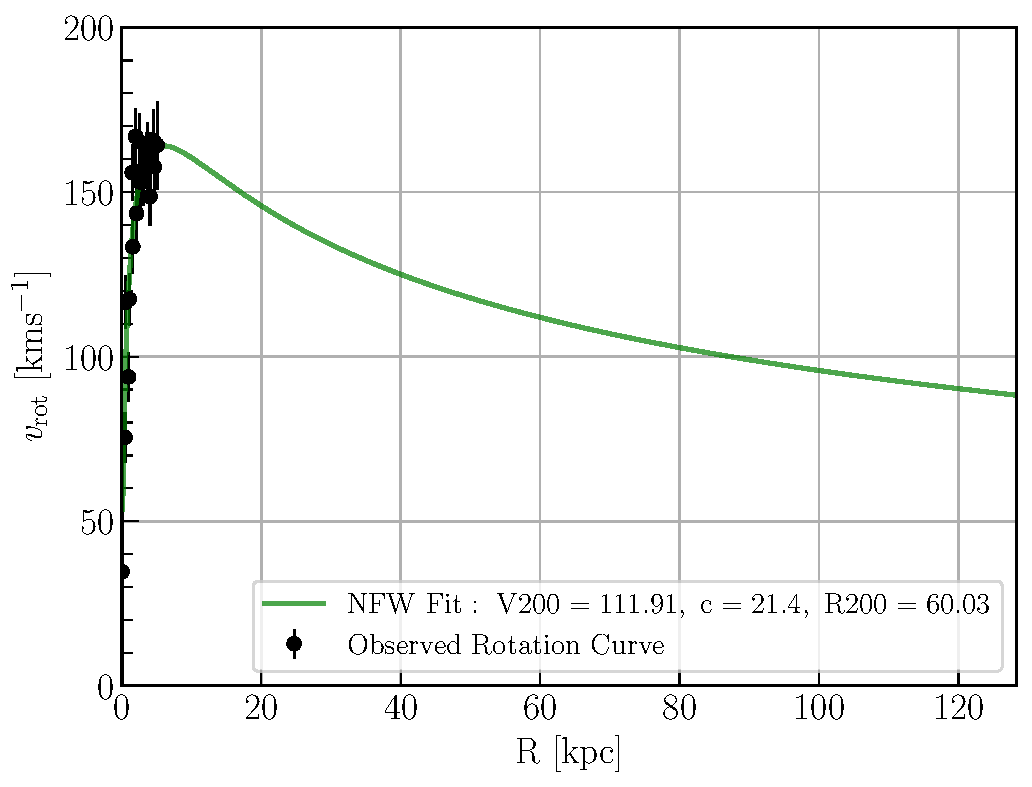
\includegraphics[width=0.319\linewidth]{NGC3633-NFW_fit_Rvir.pdf}
%        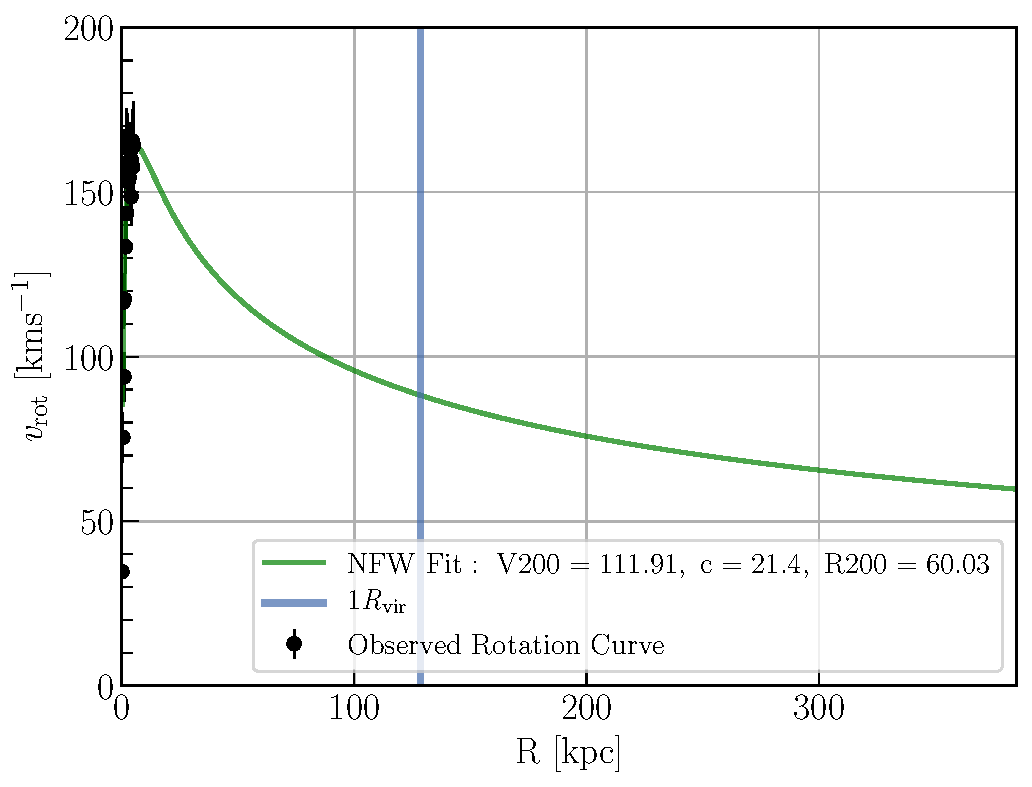
\includegraphics[width=0.319\linewidth]{NGC3633-NFW_fit_Rvir_times3_2.pdf}
%        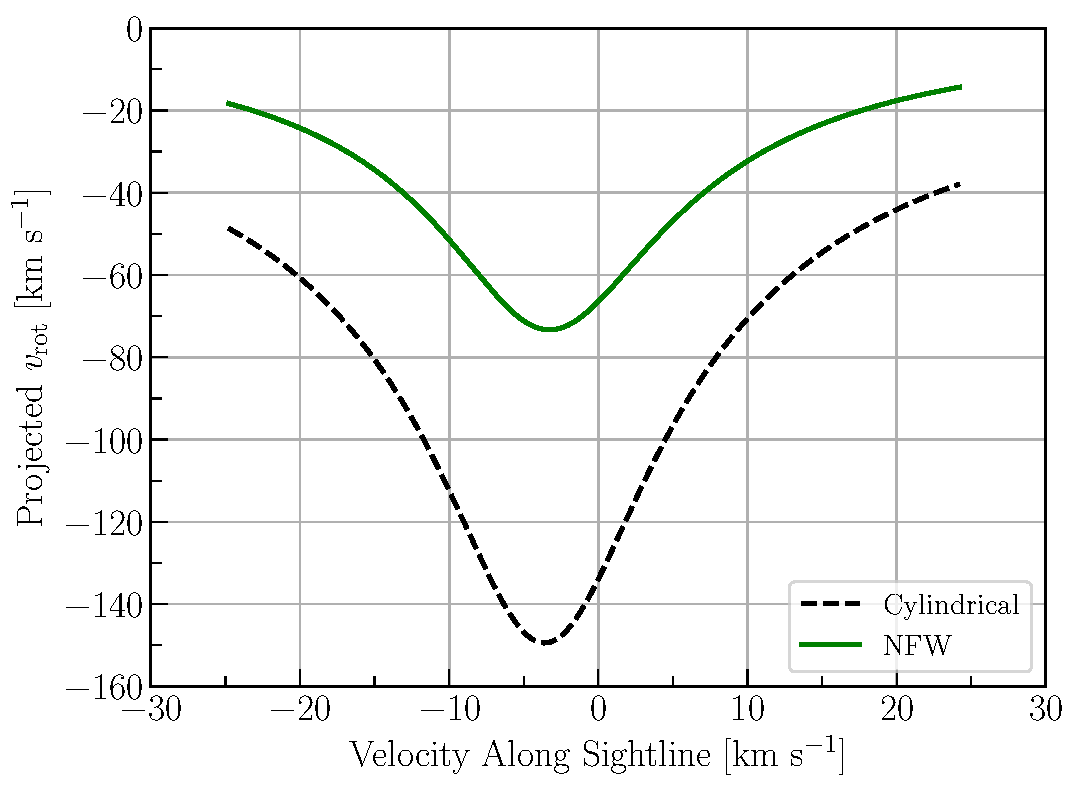
\includegraphics[width=0.331\linewidth]{NGC3633-RX_J1121_2+0326_model_plot4.pdf}
%        \caption{\small{Left: The rotation curve for NGC3633 is shown in black, with the outer 1/2 mean rotation velocity indicated in green. Our cylindrical model simply extends this green average velocity out to $3 R_{\rm vir}$.  Middle: The observed rotation curve is again shown in black, with an NFW profile fit overlaid in green. Right: The model velocity predictions for the cylindrical and NFW models are shown in dashed-black and solid-green (respectively).}}
%%        \vspace{-5pt}
%        \label{model_fits}
%        \vspace{5pt}
%\end{figure*}
%
%\begin{figure*}[h]
%        \centering
%        \vspace{0pt}
%        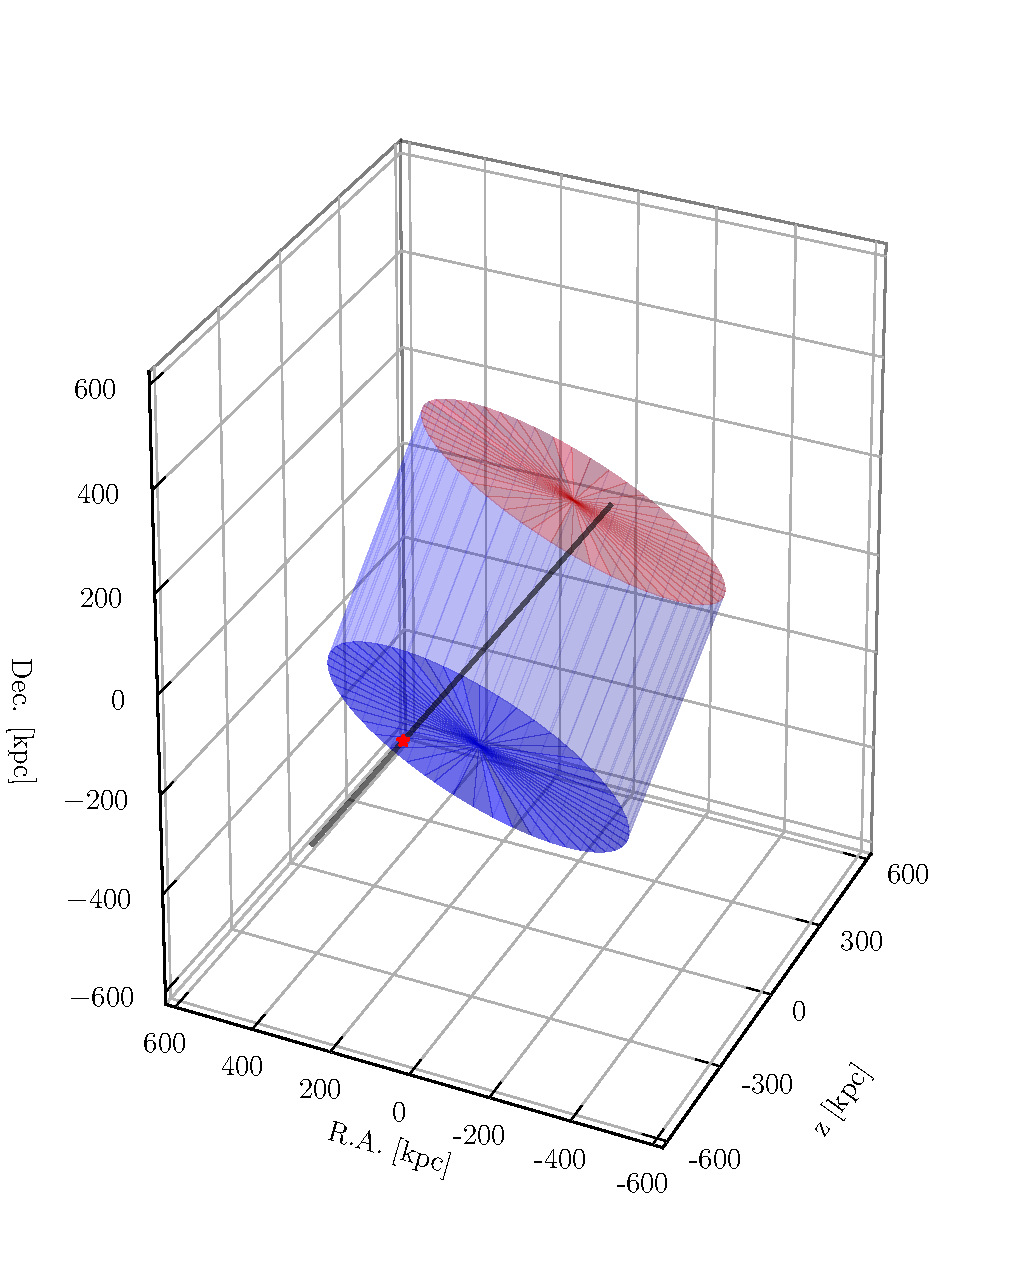
\includegraphics[width=0.32\linewidth]{NGC3633-RX_J1121_2+0326_3Dmodel_plot1_2.pdf}
%        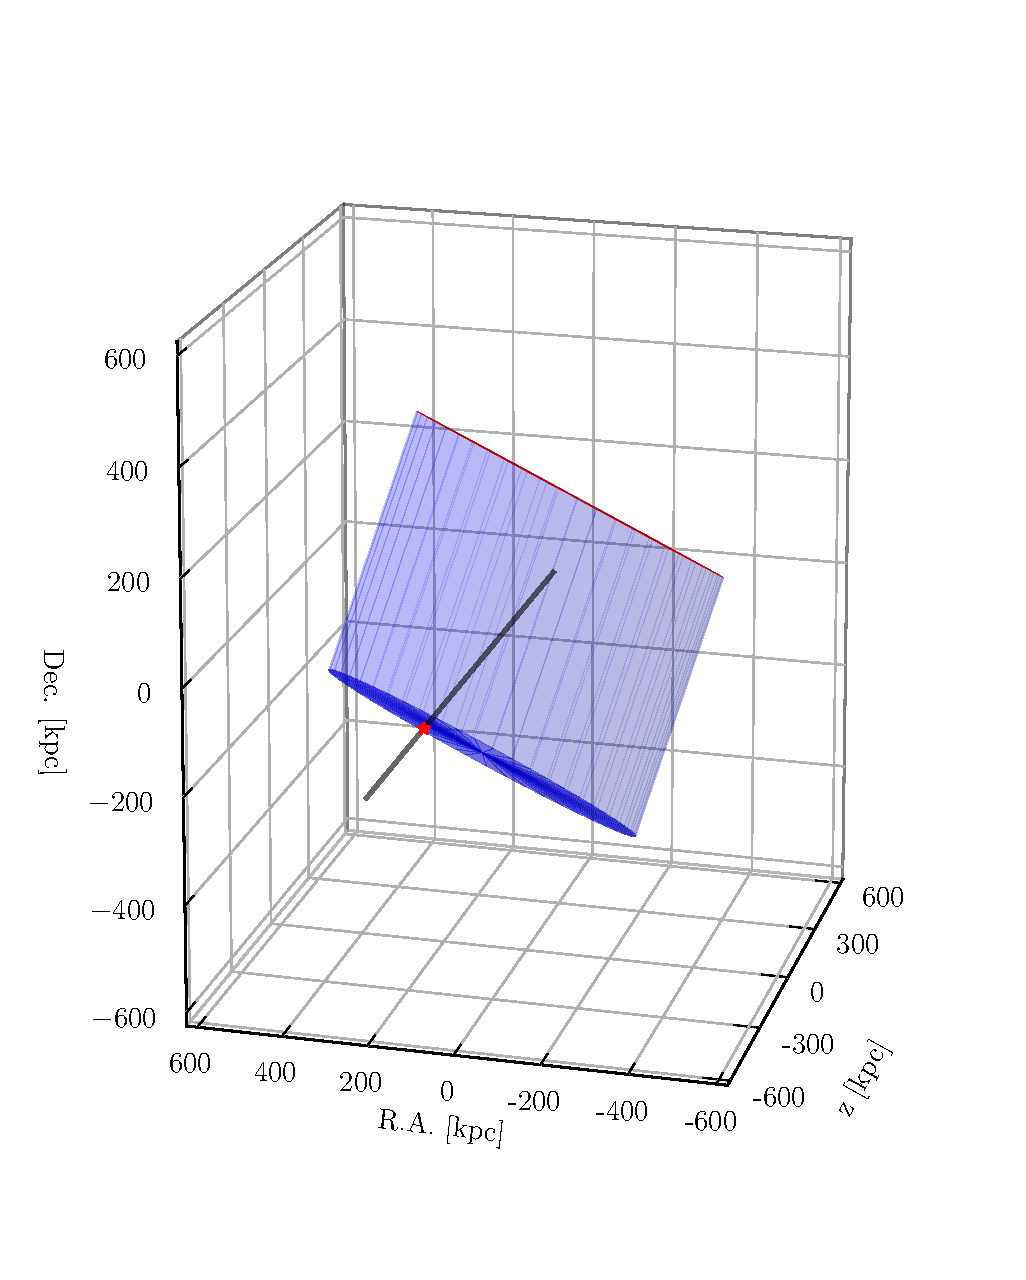
\includegraphics[width=0.32\linewidth]{NGC3633-RX_J1121_2+0326_3Dmodel_plot2_2.pdf}
%        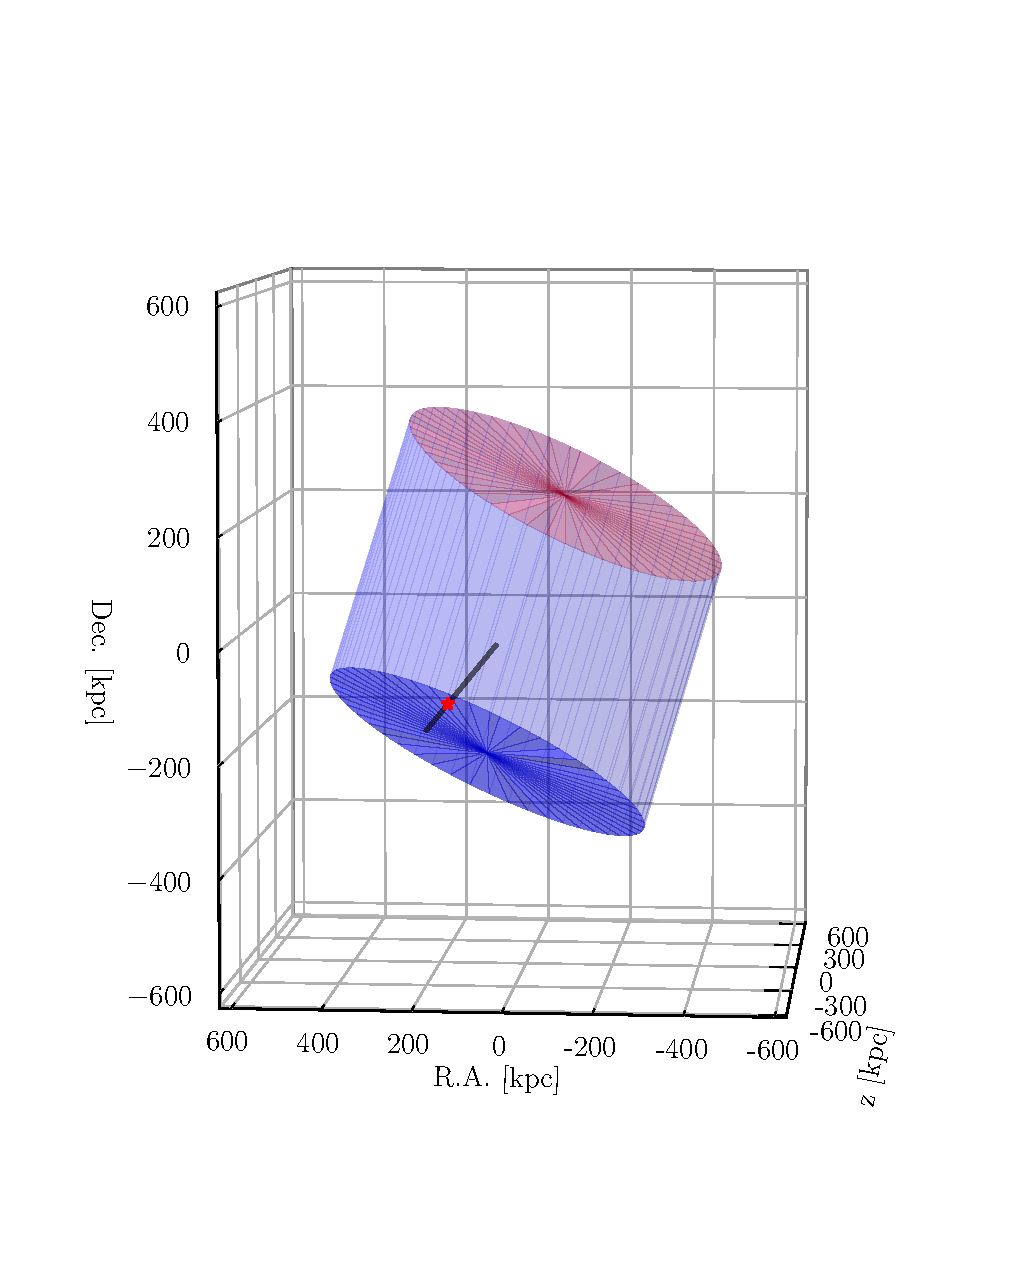
\includegraphics[width=0.32\linewidth]{NGC3633-RX_J1121_2+0326_3Dmodel_plot3_2.pdf}
%        \caption{\small{A 3D example mockup of our halo rotation model showing the orientation and extent of the NGC3633 model from 3 different viewing angles. The approaching extreme edge of the NGC3633 cylindrical halo is shown by dark-blue oval, with the far edge shown in red. The dark-grey line shows the location of the sightline toward RX\_J1121.2+0326 as it penetrates the halo, with a red star marking the first intercept point.}}
%%        \vspace{-5pt}
%        \label{3D_model}
%        \vspace{5pt}
%\end{figure*}



\section{Halo Rotation Model} \label{model}
%In order to better understand how QSO sightlines probe the intervening velocity structure we have developed a simple halo gas rotation model. 

In order to better understand how the 3D rotation of halo gas is mapped onto a 1D QSO sightline, we have developed a simple halo gas rotation model. This model is seeded by an observed rotation curve, which is then extrapolated out to a radius of $3 R_{\rm vir}$ and height of $2 R_{\rm vir}$ to form a coherently rotating halo. For each galaxy-QSO pair we create 2 rotation models: 1) a purely cylindrical halo with constant velocity from the edge of the observed rotation curve out to the edge of our $3 \times 2 R_{\rm vir}$ halo model, and 2) a cylindrical model with rotation velocities which smoothly decline as a function of radius based on a Navarro-Frenk-White (NFW) profile fit \citep{navarro1996, navarro1997}. 


For the first, purely cylindrical model, the input rotation curve is interpolated via a linear spline fit and extended out to 3$R_{vir}$ based on the average velocity of the outer 1/2 radius (see Figure \ref{model_fits}; top-left). For the second model, we fit a NFW rotation velocity profile to the input rotation curve. The form of this fit is as follows:

\begin{equation}
	V(R) = V_{200} \left [\frac{\ln(1 + c x) - c x / (1 + c x)}{x [ \ln(1 + c) - c / (1 + c)]} \right]^{\frac{1}{2}},
\end{equation}

\noindent where $x = R / R_{200}$, with $R_{200}$ being the radius at which the density contrast with respect to the critical density of the universe exceeds 200, $c = R_{200} / R_s$, with $R_s$ being the characteristic radius of the halo, and $V_{200}$ being the characteristic velocity at $R_{200}$. We have taken this form from \cite{deblok2008}. The resulting NFW fits tend to be somewhat poor toward the inner parts of the rotation curve (as has been noted by others, e.g., \citealt{cote2005}). Regardless, we are most interested in achieving a physically-motivated, declining velocity profile in the outer halo regions where most of our QSO sightlines are located, for which these fits are certainly adequate.


%\begin{figure}[h!]
%        \centering
%        \vspace{0pt}
%%        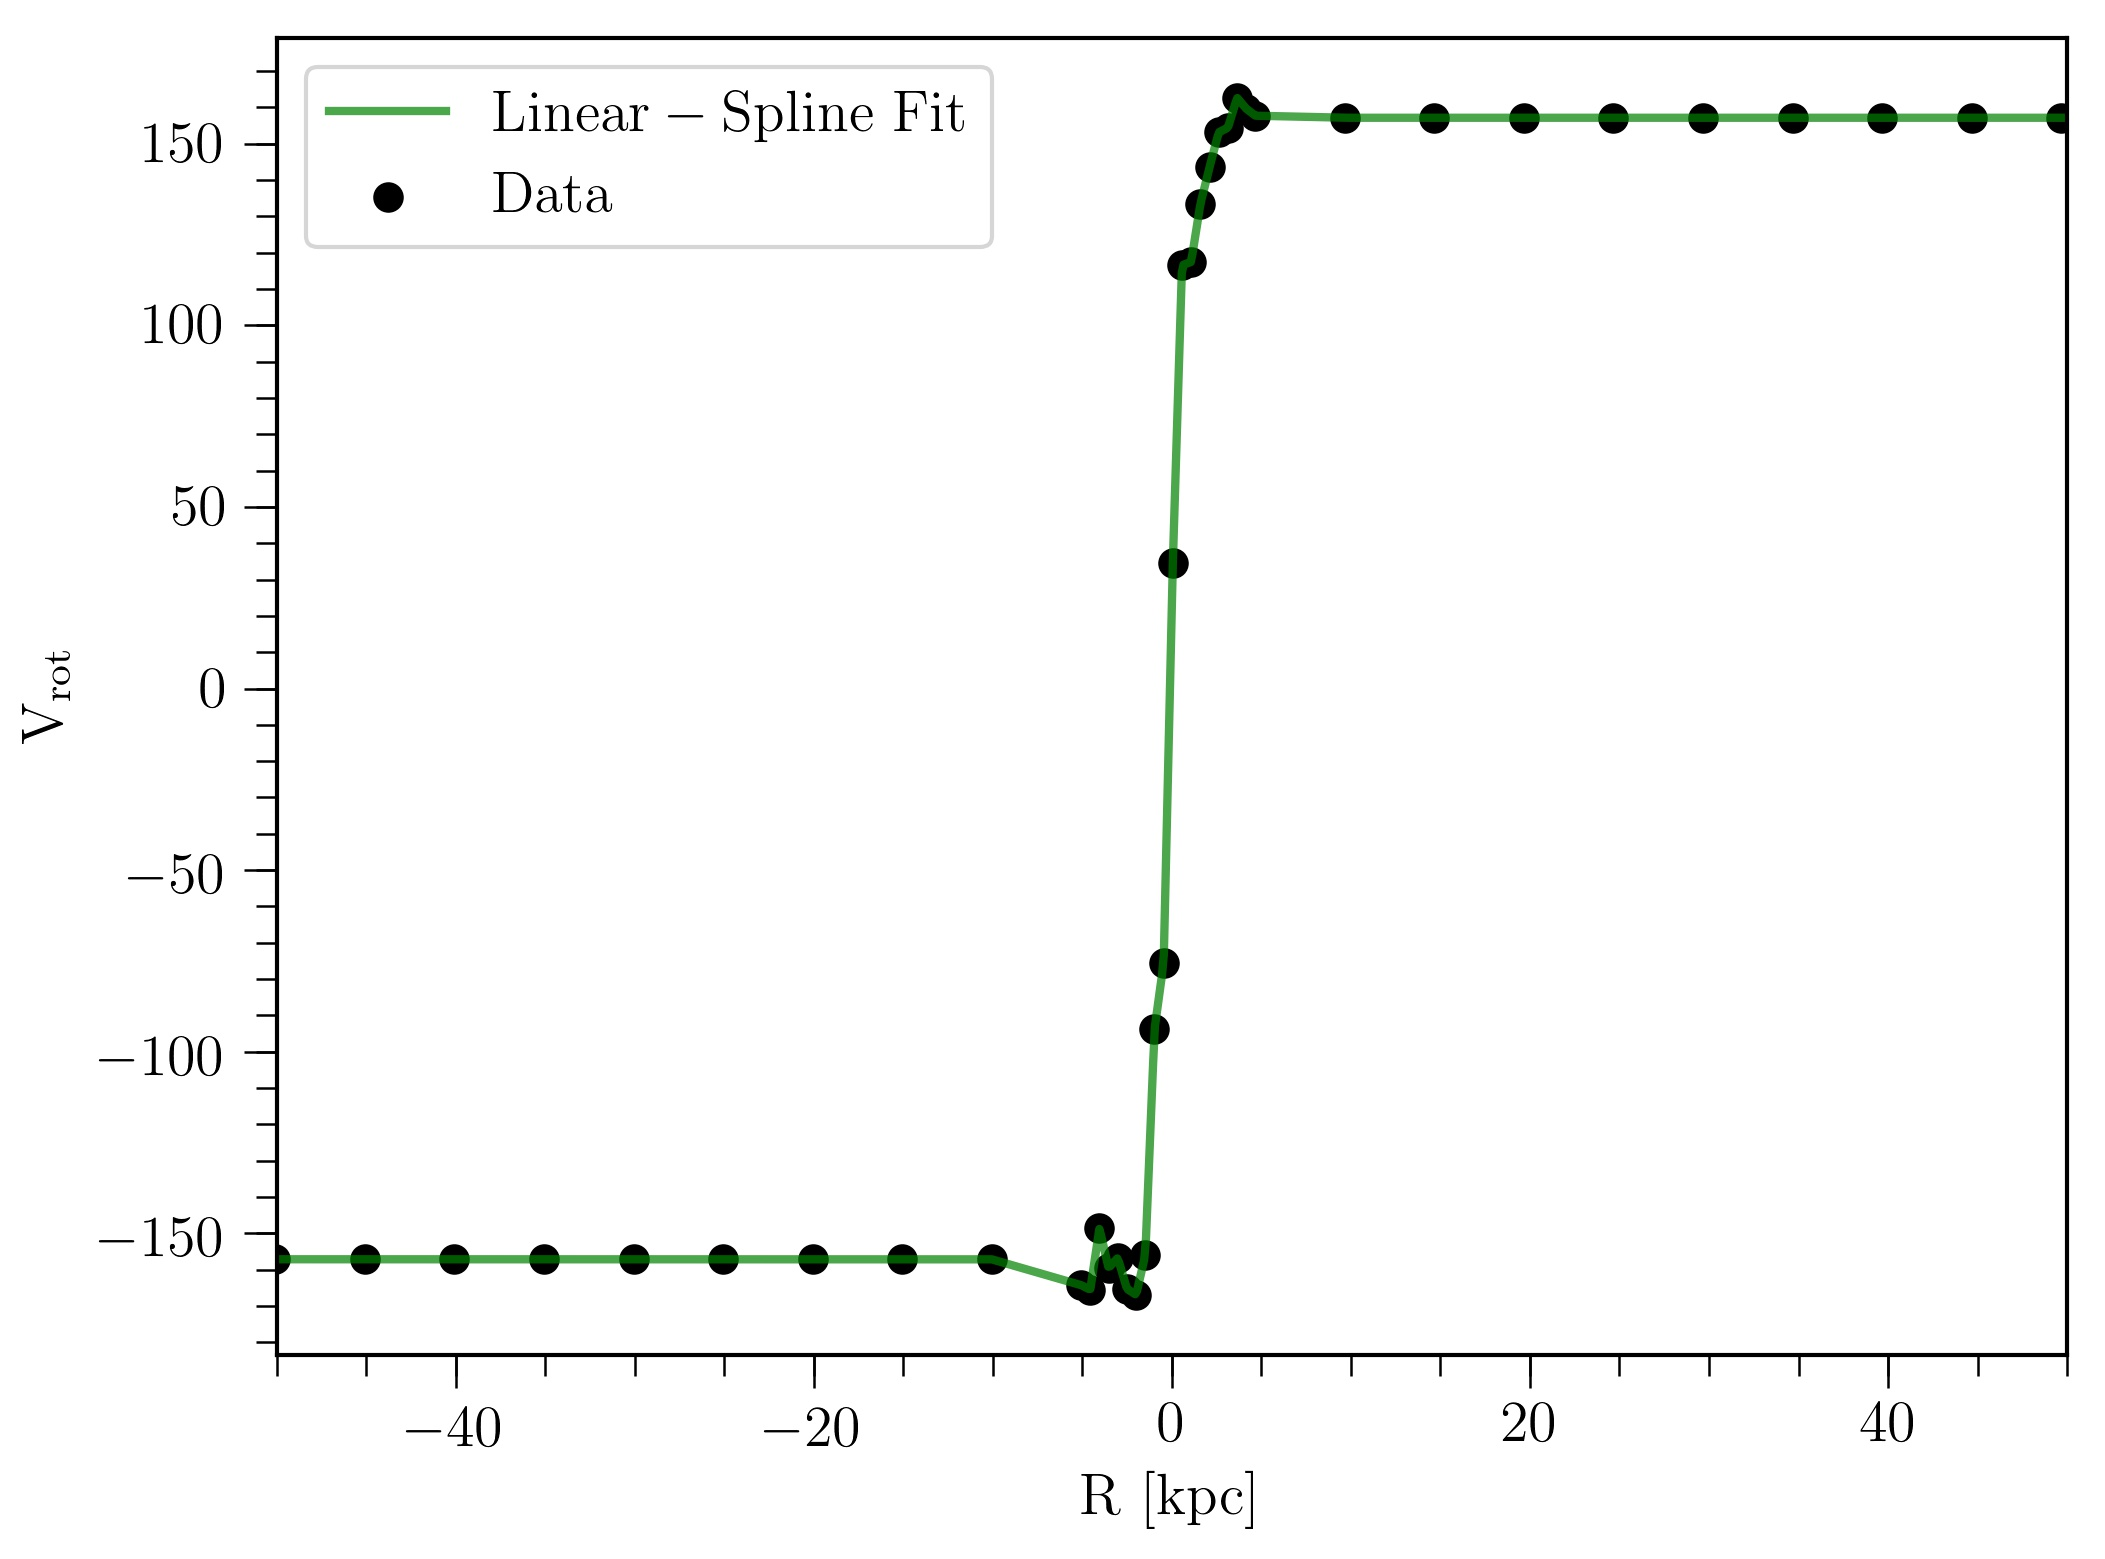
\includegraphics[width=0.36\textwidth]{NGC3633_splineFit_linear.jpg}
%        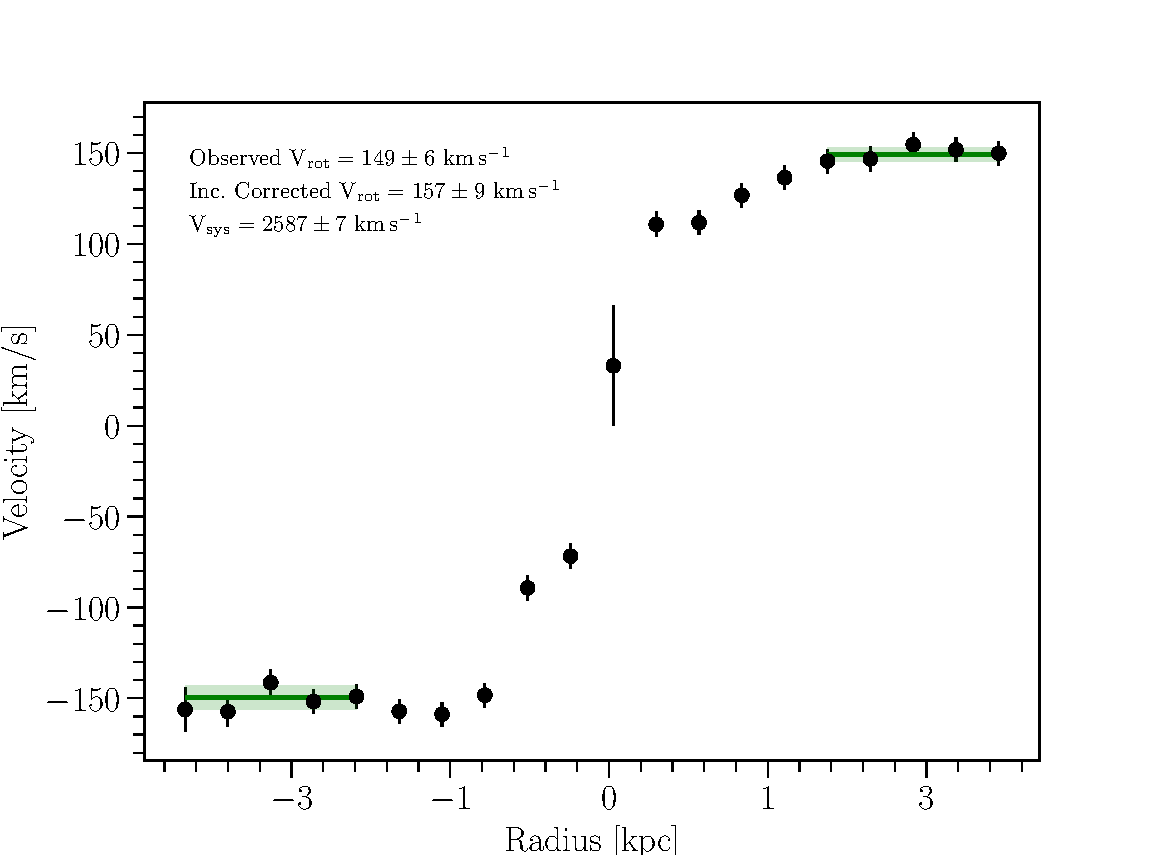
\includegraphics[width=0.9\linewidth]{NGC3633_2_rotation_curve_xphys_helio_vobs_vrotObs_new5.pdf}
%        
%        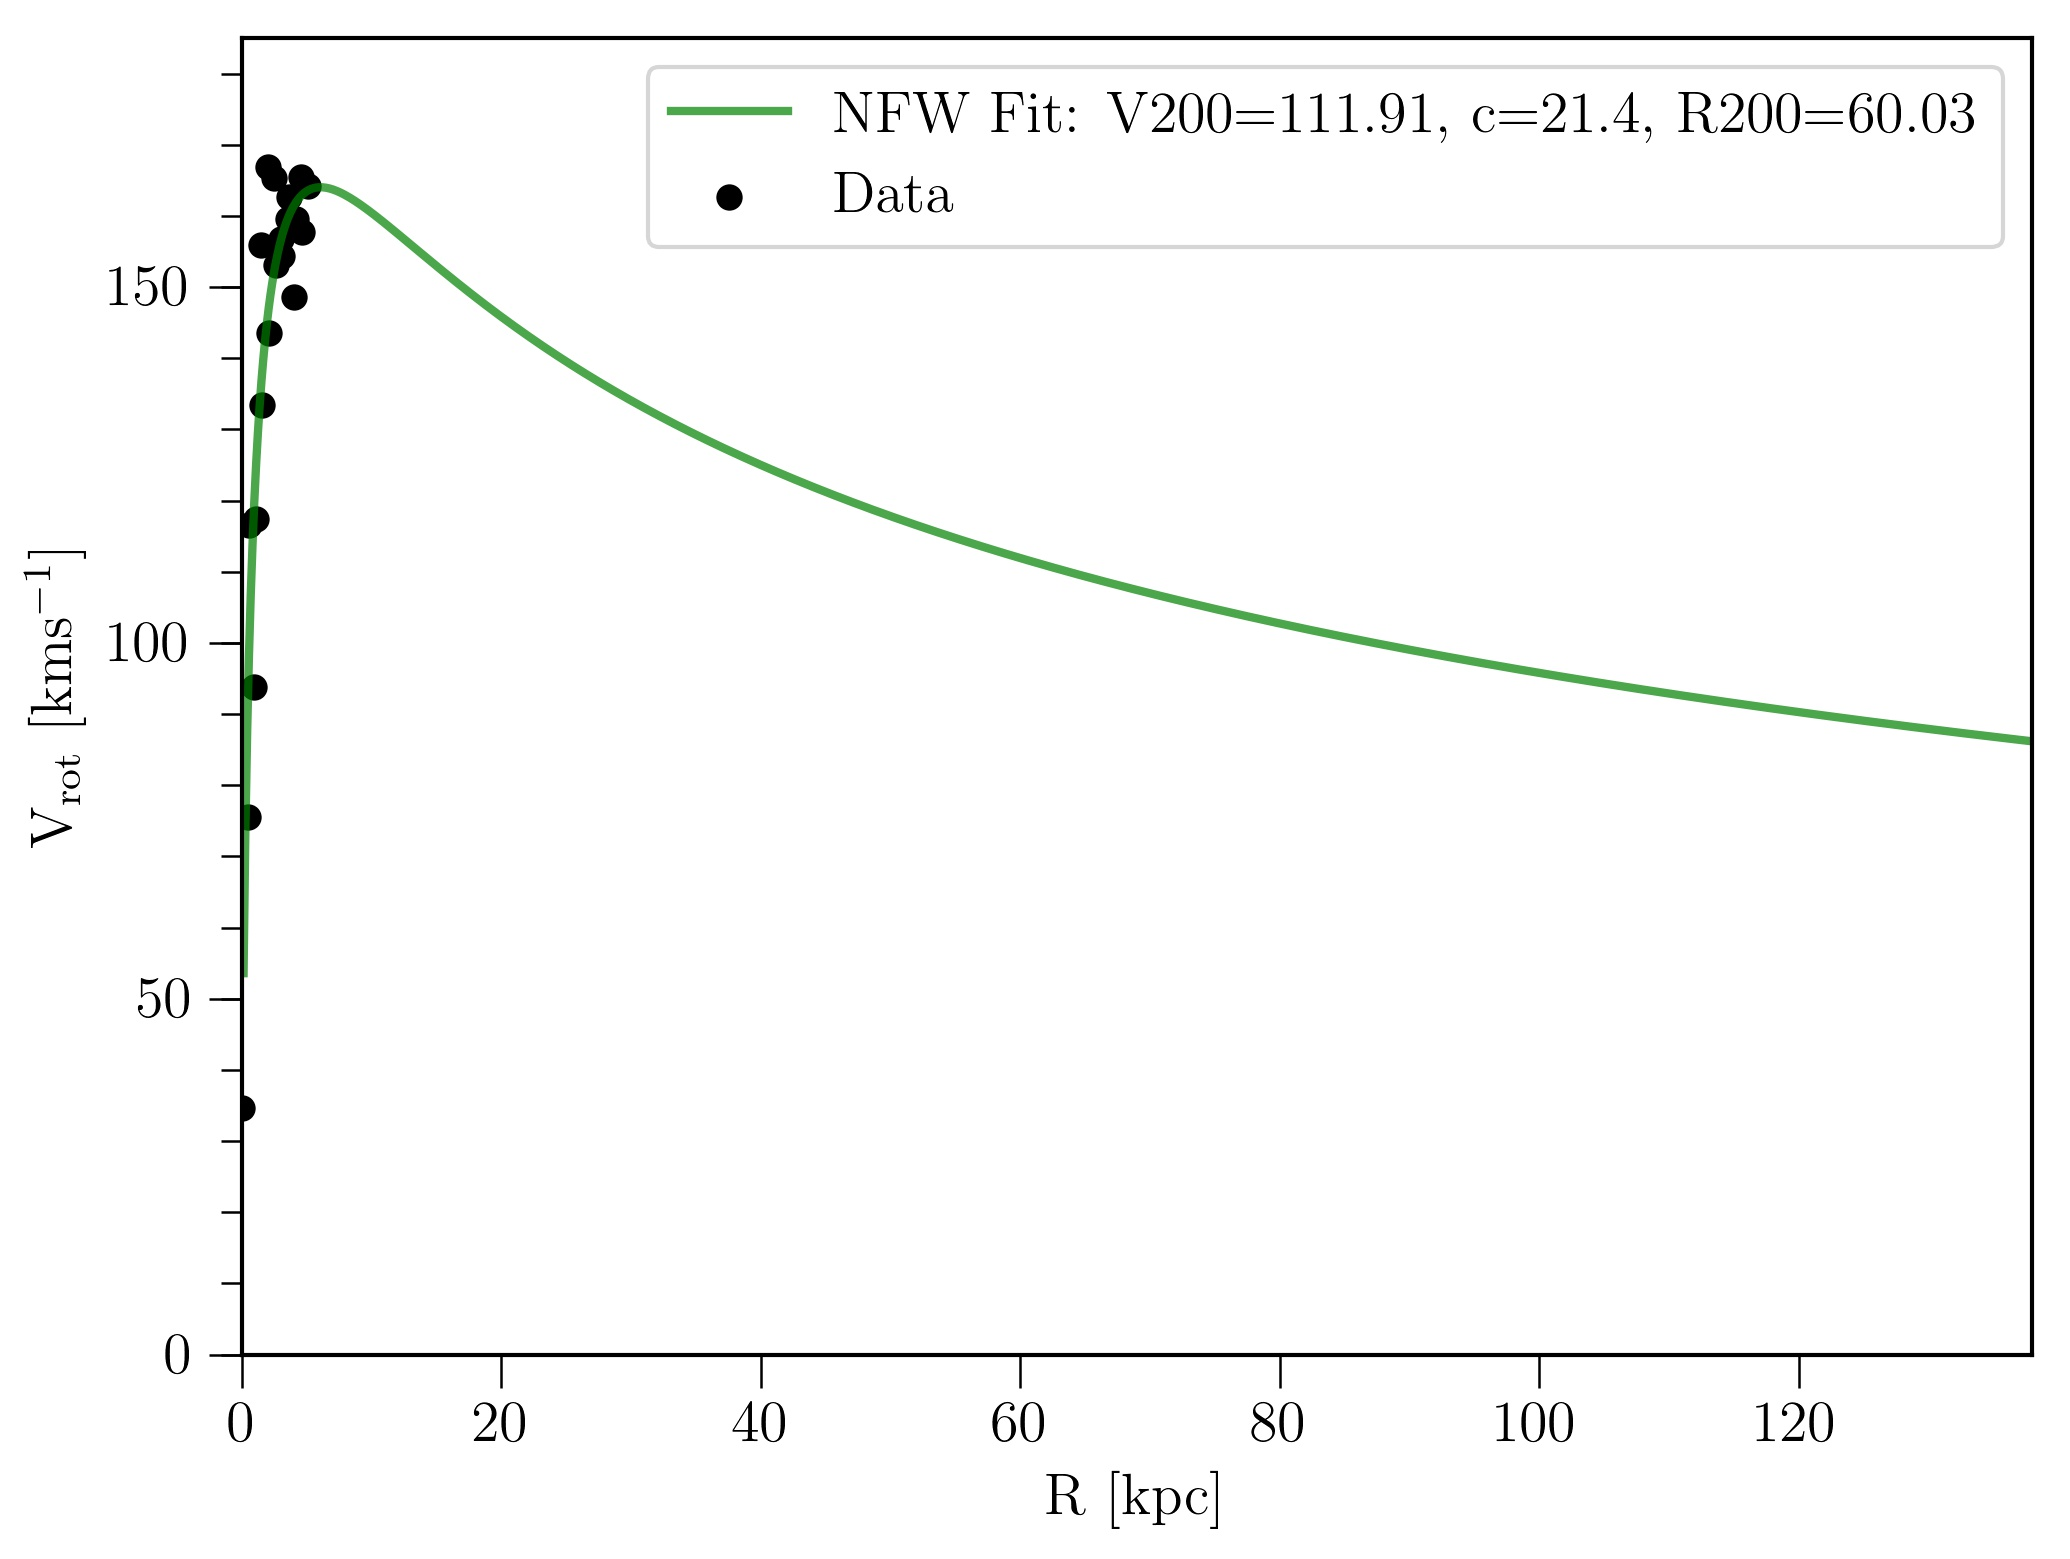
\includegraphics[width=0.9\linewidth]{NGC3633_NFW_138.jpg}
%        
%        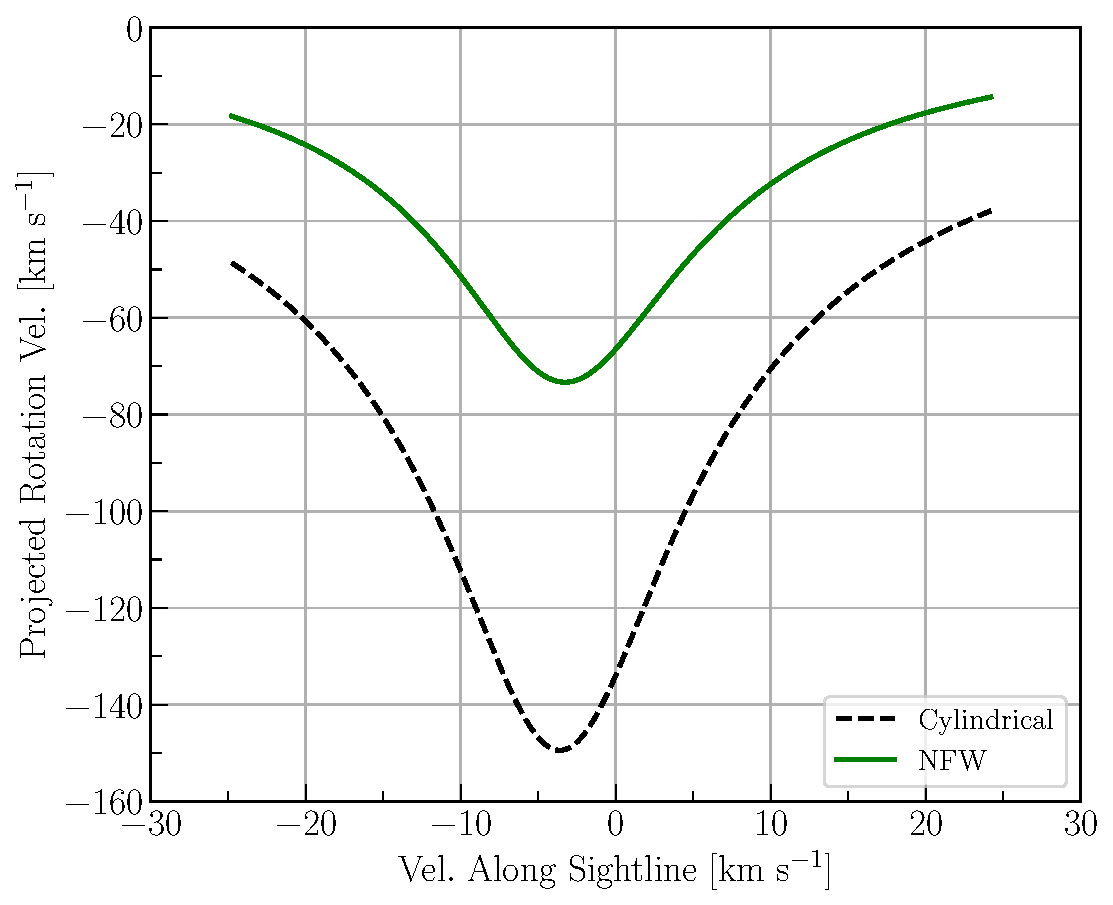
\includegraphics[width=0.9\linewidth]{NGC3633-RX_J1121_2+0326_model_plot3.pdf}
%        \caption{\small{Left: The rotation curve for NGC3633 is shown in black, with the outer 1/2 mean rotation velocity indicated in green. Our cylindrical model simply extends this green average velocity out to $3 R_{\rm vir}$.  Middle: The observed rotation curve is again shown in black, with an NFW profile fit overlaid in green. Right: The model velocity predictions for the cylindrical and NFW models are shown in dashed-black and solid-green (respectively).}}
%%        \vspace{-5pt}
%        \label{model_fits}
%        \vspace{5pt}
%\end{figure}
%
%\begin{figure}[h!]
%        \centering
%        \vspace{0pt}
%        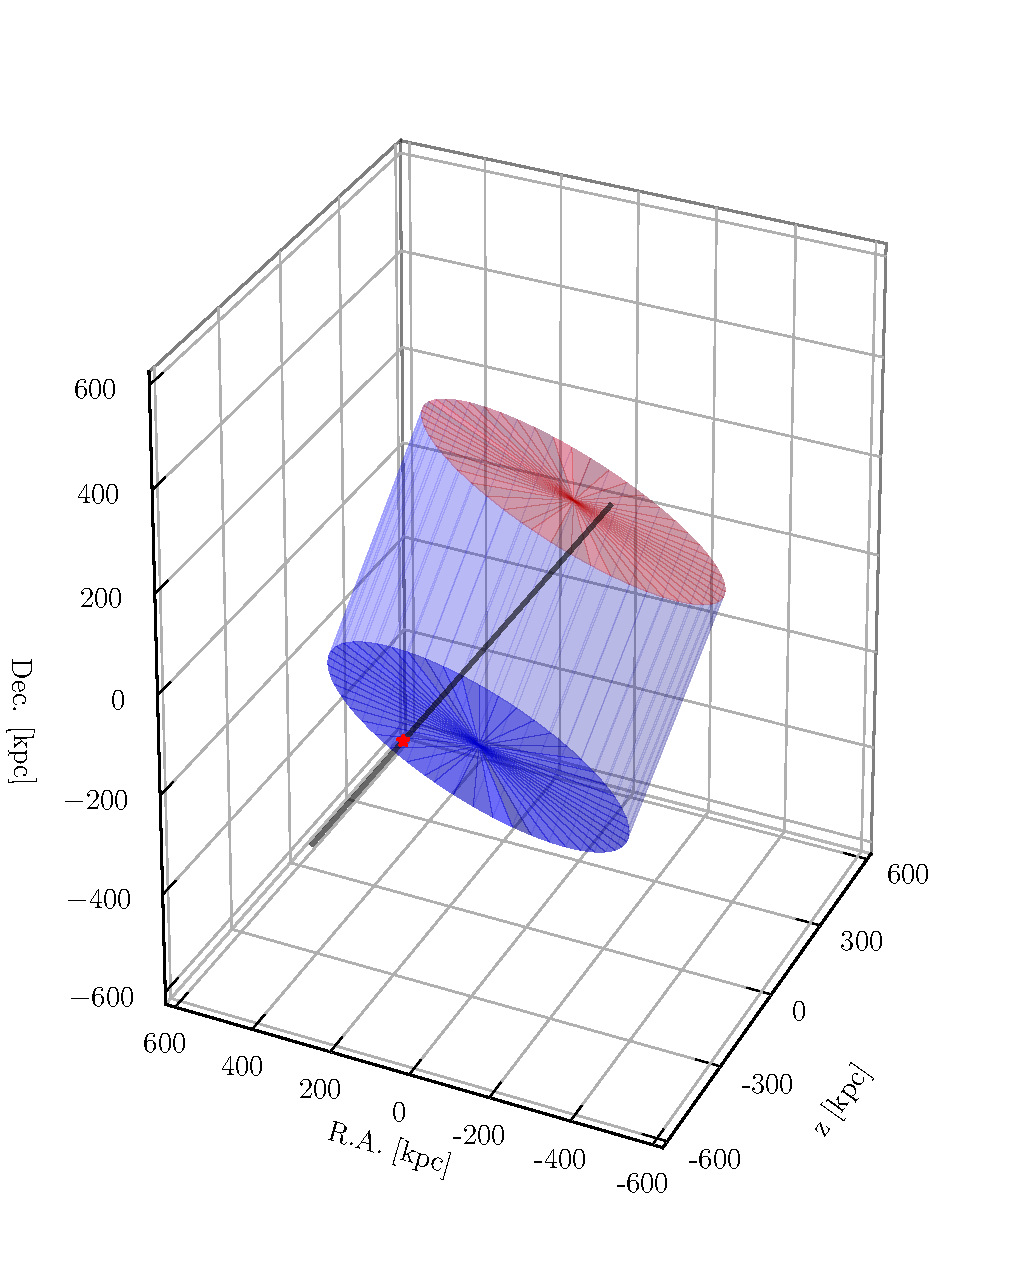
\includegraphics[width=0.6\linewidth]{NGC3633-RX_J1121_2+0326_3Dmodel_plot1_2.pdf}
%        
%        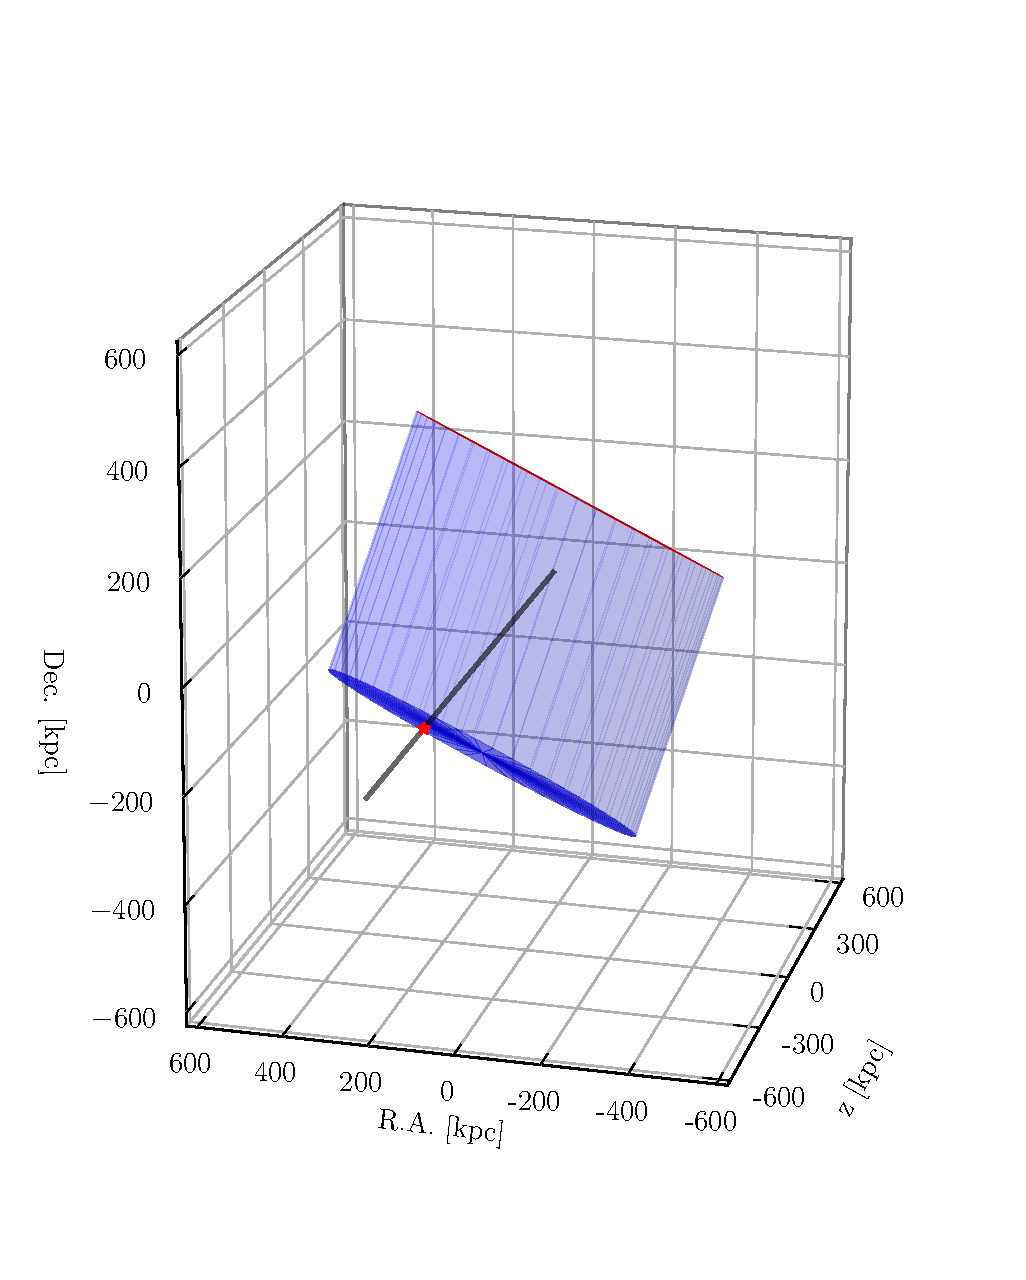
\includegraphics[width=0.6\linewidth]{NGC3633-RX_J1121_2+0326_3Dmodel_plot2_2.pdf}
%      
%        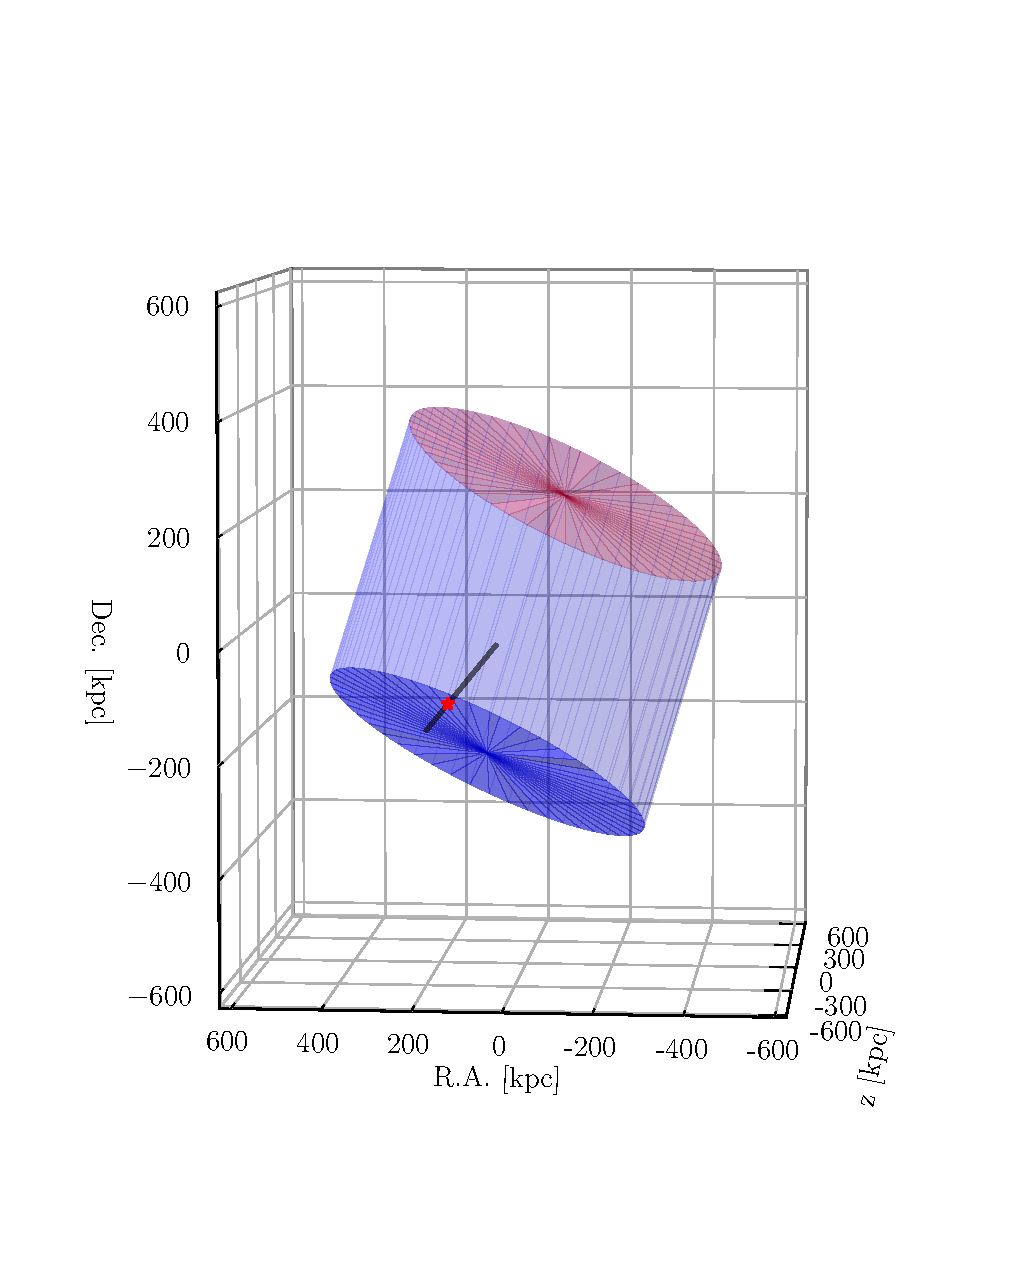
\includegraphics[width=0.6\linewidth]{NGC3633-RX_J1121_2+0326_3Dmodel_plot3_2.pdf}
%        \caption{\small{A 3D example mockup of our halo rotation model showing the orientation and extent of the NGC3633 model from 3 different viewing angles. The approaching extreme edge of the NGC3633 cylindrical halo is shown by dark-blue oval, with the far edge shown in red. The dark-grey line shows the location of the sightline toward RX\_J1121.2+0326 as it penetrates the halo, with a red star marking the first intercept point.}}
%%        \vspace{-5pt}
%        \label{3D_model}
%        \vspace{5pt}
%\end{figure}

 

Next, we project the interpolated rotation curve and NFW fit onto a plane oriented to a mock QSO sightline identically to the input galaxy-QSO pair orientation. By then stacking multiple such rotation-planes along the galaxy z-axis direction, we build a simple cylindrical halo model embedded with the fit and interpolated rotation curve. Finally, we calculate the projected rotation velocity encountered at each position along the sightline. The result is a function representing the rotation velocity encountered by the sightline as a function of velocity (i.e., distance) along it. Each model produces the velocity a co-rotating absorber would project onto the spectrum as a function of velocity along the sightline. Of course, there is an inherent degeneracy between the projected rotation velocity and the velocity along the sightline. For example, a stationary (not co-rotating) absorber located blueward of the galaxy systemic velocity would be indistinguishable from an approaching, co-rotating absorber physically located at the galaxy systemic velocity. 

We then collapse this into the range of possible observed velocities by summing the x- and y-velocity ranges generated by each model. This has the effect of combining \emph{both} the projected rotation velocity \emph{and} the physical velocity separation between an absorber and the galaxy's heliocentric velocity ($\Delta v = v_{\rm absorber} - v_{\rm galaxy}$) into a single velocity range, which we then can compare to the measured absorption velocity ($v_{\rm Ly\alpha}$). This resulting velocity range also includes the $1-\sigma$ rotation curve error estimates as given in the $v_{\rm rot}$ column of Table \ref{models}.

Figures \ref{model_fits} illustrates an example model for the SALT-observed galaxy NGC3633, with our observed rotation curve, the NFW fit, and the resulting cylindrical and NFW model output velocity distributions from left-to-right on top, and a 3-D halo mockup from 3 different viewing angles on the bottom. In most cases, and as seen in this example, the two model outputs have similar \emph{shape}, but the NFW profile fit usually results in a lower velocity range (i.e., closer to systemic). Because we combine projected velocity with velocity along the sightline, many models allow for an absorber to have the wrong sign of $\Delta v$. For example, an absorber on the approaching side of a halo but at the distant edge would end up with a range of positive $\Delta v$ consistent with co-rotation because the relatively positive redshift component overcomes the relatively negative rotation component. The result is that some absorbers with the ``wrong" on-sky velocity for co-rotation are indeed consistent with co-rotation based on our models.

% NFW profile comes from de Blok 2008


\startlongtable
\begin{deluxetable*}{l l l r r r r r r r r}
%\rotate
\tabletypesize{\scriptsize}
\tablewidth{0pt}
\tablecaption{Halo Model Results and Ly$\alpha$ Absorption Properties\label{models}}
\tablehead{
\colhead{$\#$}	&\colhead{Galaxy}  	&  \colhead{Target} 	&  \colhead{$\rho$ }  &  \colhead{Az.}      & \colhead{$v_{\rm sys}$}&  \colhead{$v_{\rm rot}$\tablenotemark{a}}   &  \colhead{$v_{\rm Ly\alpha}$} & \colhead{$W_{\rm Ly\alpha}$} & \colhead{Cyl. Model\tablenotemark{b}}  & \colhead{NFW Model\tablenotemark{c}}  \\
			  				&				&          			&  \colhead{(kpc)}   & \colhead{(deg)}	& \colhead{(\kms)}	     & \colhead{(\kms)}  		& \colhead{(\kms)}  		      	&  \colhead{(m\AA)}  			  & \colhead{(\kms)} 	       & \colhead{(\kms)} }
\colnumbers
\startdata
1  &        CGCG039-137  &   RX\_J1121.2+0326  &         99  &     71  &  6918  &      $143 \pm 25$  &  6975  &           678  &            6881 - 7079  & 6881 - 7106  \\
2  &        ESO343-G014  &   RBS1768  &                 466  &    74  &  9139  &      $-205 \pm 32$  & 9308  &           63  &             8904 - 9155  & 8985 - 9176  \\
2  &        ESO343-G014  &   RBS1768  &                 466  &    74  &  9139  &      $-205 \pm 32$  & 9360  &           306  &            8904 - 9155  & 8985 - 9176  \\
2  &        ESO343-G014  &   RBS1768  &                 466  &    74  &  9139  &      $-205 \pm 32$  & 9434  &           161  &            8904 - 9155  & 8985 - 9176  \\
3  &        IC5325  &        RBS2000  &                 314  &    64  &  1512  &      $-125 \pm 27$  & 1598  &           35  &             1467 - 1499  & 1479 - 1520  \\
4  &        MCG-03-58-009  & MRC2251-178  &             355  &    71  &  9015  &      $171 \pm 22$  &  9029  &           62  &             8985 - 9171  & 8969 - 9117  \\
5  &        NGC1566  &       1H0419-577  &              303  &    10  &  1502  &      $195 \pm 47$  &  1075  &           249  &            1534 - 1592  & 1485 - 1547  \\
5  &        NGC1566  &       1H0419-577  &              303  &    10  &  1502  &      $195 \pm 47$  &  1123  &           269  &            1534 - 1592  & 1485 - 1547  \\
5  &        NGC1566  &       1H0419-577  &              303  &    10  &  1502  &      $195 \pm 47$  &  1188  &           240  &            1534 - 1592  & 1485 - 1547  \\
5  &        NGC1566  &       1H0419-577  &              303  &    10  &  1502  &      $195 \pm 47$  &  1264  &           91  &             1534 - 1592  & 1485 - 1547  \\
5  &        NGC1566  &       1H0419-577  &              303  &    10  &  1502  &      $195 \pm 47$  &  2020  &           9  &              1534 - 1592  & 1485 - 1547  \\
6  &        NGC1566  &       HE0429-5343  &             256  &    60  &  1502  &      $-195 \pm 47$  & 1167  &           79  &             1439 - 1506  & 1470 - 1525  \\
6  &        NGC1566  &       HE0429-5343  &             256  &    60  &  1502  &      $-195 \pm 47$  & 1358  &           136  &            1439 - 1506  & 1470 - 1525  \\
7  &        NGC2770  &       FBQSJ0908+3246  &          204  &    59  &  1948  &      $148 \pm 6$  &   1915  &           202  &            1798 - 1946  & 1825 - 1959  \\
7  &        NGC2770  &       FBQSJ0908+3246  &          204  &    59  &  1948  &      $148 \pm 6$  &   1982  &           230  &            1798 - 1946  & 1825 - 1959  \\
8  &        NGC2770  &       TON1009  &                 267  &    41  &  1948  &      $148 \pm 6$  &   1908  &           111  &            1798 - 1912  & 1832 - 1937  \\
8  &        NGC2770  &       TON1009  &                 267  &    41  &  1948  &      $148 \pm 6$  &   1980  &           243  &            1798 - 1912  & 1832 - 1937  \\
9  &        NGC2770  &       TON1015  &                 218  &    61  &  1948  &      $148 \pm 6$  &   1833  &           244  &            1949 - 2097  & 1936 - 2069  \\
9  &        NGC2770  &       TON1015  &                 218  &    61  &  1948  &      $148 \pm 6$  &   1985  &           80  &             1949 - 2097  & 1936 - 2069  \\
10  &       NGC2770  &       SDSSJ091052.80+333008.0  & 239  &    66  &  1948  &      $148 \pm 6$  &   1824  &           266  &            1952 - 2097  & 1939 - 2066  \\
10  &       NGC2770  &       SDSSJ091052.80+333008.0  & 239  &    66  &  1948  &      $148 \pm 6$  &   1975  &           68  &             1952 - 2097  & 1939 - 2066  \\
11  &       NGC2770  &       SDSSJ091127.30+325337.0  & 234  &    30  &  1948  &      $148 \pm 6$  &   2063  &           271  &            1794 - 1909  & 1825 - 1932  \\
12  &       NGC3067  &       3C232  &                   11  &     74  &  1465  &      $143 \pm 9$  &   1408  &           2092  &           1336 - 1490  & 1318 - 1491  \\
12  &       NGC3067  &       3C232  &                   11  &     74  &  1465  &      $143 \pm 9$  &   1510  &           700  &            1336 - 1490  & 1318 - 1491  \\
12  &       NGC3067  &       3C232  &                   11  &     74  &  1465  &      $143 \pm 9$  &   1641  &           1635  &           1336 - 1490  & 1318 - 1491  \\
13  &       NGC3067  &       SDSSJ095914.80+320357.0  & 128  &    43  &  1465  &      $143 \pm 9$  &   1493  &           623  &            1472 - 1607  & 1451 - 1555  \\
14  &       NGC3198  &       RX\_J1017.5+4702  &         370  &    55  &  660  &       $152 \pm 5$  &   629  &            71  &             502 - 641  &   565 - 668  \\
15  &       NGC3351  &       SDSSJ104335.90+115129.0  & 31  &     43  &  778  &       $199 \pm 16$  &  717  &            823  &            632 - 797  &   670 - 804  \\
15  &       NGC3351  &       SDSSJ104335.90+115129.0  & 31  &     43  &  778  &       $199 \pm 16$  &  882  &            621  &            632 - 797  &   670 - 804  \\
15  &       NGC3351  &       SDSSJ104335.90+115129.0  & 31  &     43  &  778  &       $199 \pm 16$  &  1030  &           391  &            632 - 797  &   670 - 804  \\
16  &       NGC3432  &       CSO295  &                  20  &     82  &  617  &       $119 \pm 8$  &   600  &            568  &            580 - 670  &   580 - 759  \\
16  &       NGC3432  &       CSO295  &                  20  &     82  &  616  &       $119 \pm 8$  &   662  &            585  &            579 - 669  &   579 - 758  \\
17  &       NGC3432  &       RX\_J1054.2+3511  &         290  &    57  &  616  &       $119 \pm 8$  &   703  &            184  &            613 - 744  &   605 - 735  \\
18  &       NGC3513  &       H1101-232  &               60  &     67  &  1204  &      $22 \pm 24$  &   1182  &           635  &            1182 - 1233  & 1183 - 1233  \\
19  &       NGC3631  &       RX\_J1117.6+5301  &         78  &     75  &  1156  &      $143 \pm 25$  &  1131  &           374  &            1163 - 1186  & 1150 - 1178  \\
19  &       NGC3631  &       RX\_J1117.6+5301  &         78  &     75  &  1156  &      $143 \pm 25$  &  1259  &           62  &             1163 - 1186  & 1150 - 1178  \\
20  &       NGC3631  &       SBS1116+523  &             163  &    40  &  1156  &      $143 \pm 25$  &  -99  &            -99  &            1094 - 1156  & 1118 - 1171  \\
21  &       NGC3631  &       SDSSJ111443.70+525834.0  & 145  &    72  &  1156  &      $143 \pm 25$  &  1163  &           232  &            1160 - 1187  & 1147 - 1181  \\
22  &       NGC3631  &       SDSSJ112448.30+531818.0  & 86  &     74  &  1156  &      $143 \pm 25$  &  1019  &           71  &             1129 - 1148  & 1133 - 1163  \\
22  &       NGC3631  &       SDSSJ112448.30+531818.0  & 86  &     74  &  1156  &      $143 \pm 25$  &  1141  &           165  &            1129 - 1148  & 1133 - 1163  \\
23  &       NGC3633  &       RX\_J1121.2+0326  &         184  &    58  &  2587  &      $-157 \pm 9$  &  2605  &           180  &            2425 - 2576  & 2502 - 2599  \\
24  &       NGC3666  &       SDSSJ112439.50+113117.0  & 58  &     83  &  1060  &      $127 \pm 6$  &   1047  &           345  &            967 - 1080  &  914 - 1080  \\
24  &       NGC3666  &       SDSSJ112439.50+113117.0  & 58  &     83  &  1060  &      $127 \pm 6$  &   1099  &           272  &            967 - 1080  &  914 - 1080  \\
25  &       NGC3726  &       CSO1208  &                 369  &    88  &  866  &       $162 \pm 10$  &  731  &            470  &            839 - 895  &   837 - 888  \\
25  &       NGC3726  &       CSO1208  &                 369  &    88  &  866  &       $162 \pm 10$  &  874  &            506  &            839 - 895  &   837 - 888  \\
26  &       NGC3726  &       RX\_J1142.7+4625  &         440  &    86  &  866  &       $162 \pm 10$  &  818  &            375  &            832 - 854  &   836 - 861  \\
27  &       NGC4529  &       MRK771  &                  159  &    23  &  2536  &      $106 \pm 15$  &  2553  &           240  &            2416 - 2503  & 2432 - 2517  \\
28  &       NGC4536  &       3C273.0  &                 349  &    11  &  1867  &      $148 \pm 39$  &  1580  &           369  &            1930 - 2022  & 1841 - 1926  \\
28  &       NGC4536  &       3C273.0  &                 349  &    11  &  1867  &      $148 \pm 39$  &  2156  &           42  &             1930 - 2022  & 1841 - 1926  \\
28  &       NGC4536  &       3C273.0  &                 349  &    11  &  1867  &      $148 \pm 39$  &  2267  &           27  &             1930 - 2022  & 1841 - 1926  \\
29  &       NGC4536  &       HE1228+0131  &             338  &    51  &  1867  &      $148 \pm 39$  &  1495  &           160  &            1881 - 1935  & 1856 - 1900  \\
29  &       NGC4536  &       HE1228+0131  &             338  &    51  &  1867  &      $148 \pm 39$  &  1571  &           23  &             1881 - 1935  & 1856 - 1900  \\
29  &       NGC4536  &       HE1228+0131  &             338  &    51  &  1867  &      $148 \pm 39$  &  1686  &           321  &            1881 - 1935  & 1856 - 1900  \\
29  &       NGC4536  &       HE1228+0131  &             338  &    51  &  1867  &      $148 \pm 39$  &  1721  &           303  &            1881 - 1935  & 1856 - 1900  \\
29  &       NGC4536  &       HE1228+0131  &             338  &    51  &  1867  &      $148 \pm 39$  &  1854  &           78  &             1881 - 1935  & 1856 - 1900  \\
30  &       NGC4565  &       RX\_J1236.0+2641  &         147  &    41  &  1230  &      $253 \pm 12$  &  1009  &           365  &            1228 - 1495  & 1199 - 1390  \\
30  &       NGC4565  &       RX\_J1236.0+2641  &         147  &    41  &  1230  &      $253 \pm 12$  &  1166  &           305  &            1228 - 1495  & 1199 - 1390  \\
30  &       NGC4565  &       RX\_J1236.0+2641  &         147  &    41  &  1230  &      $253 \pm 12$  &  1254  &           122  &            1228 - 1495  & 1199 - 1390  \\
31  &       NGC4939  &       PG1302-102  &              254  &    61  &  3093  &      $-234 \pm 39$  & 3448  &           72  &             2845 - 3109  & 2942 - 3131  \\
32  &       NGC5364  &       SDSSJ135726.27+043541.4  & 165  &    84  &  1238  &      $155 \pm 23$  &  967  &            348  &            1211 - 1370  & 1207 - 1324  \\
32  &       NGC5364  &       SDSSJ135726.27+043541.4  & 165  &    84  &  1238  &      $155 \pm 23$  &  1124  &           83  &             1211 - 1370  & 1207 - 1324  \\
33  &       NGC5786  &       QSO1500-4140  &            453  &    1  &   2975  &      $172 \pm 25$  &  3138  &           177  &            3062 - 3157  & 2975 - 3060  \\
34  &       NGC5907  &       SBS1503+570  &             413  &    47  &  667  &       $229 \pm 6$  &   708  &            301  &            696 - 903  &   641 - 774  \\
35  &       NGC5907  &       RBS1503  &                 478  &    63  &  667  &       $229 \pm 6$  &   -99  &            -99  &            432 - 659  &   565 - 701  \\
36  &       NGC5951  &       2E1530+1511  &             55  &     85  &  1780  &      $133 \pm 6$  &   1795  &           507  &            1748 - 1902  & 1748 - 1909  \\
36  &       NGC5951  &       2E1530+1511  &             55  &     85  &  1780  &      $133 \pm 6$  &   1953  &           137  &            1748 - 1902  & 1748 - 1909  \\
37  &       NGC6140  &       MRK876  &                  113  &    21  &  910  &       $138 \pm 5$  &   939  &            379  &            952 - 1021  &  948 - 1023  \\
38  &       NGC7817  &       MRK335  &                  343  &    90  &  2309  &      $178 \pm 6$  &   1954  &           216  &            2283 - 2284  & 2283 - 2285  \\
38  &       NGC7817  &       MRK335  &                  343  &    90  &  2309  &      $178 \pm 6$  &   2274  &           150  &            2283 - 2284  & 2283 - 2285  \\
39  &       UGC04238  &      PG0804+761  &              148  &    59  &  1544  &      $92 \pm 12$  &   1526  &           62  &             1538 - 1642  & 1532 - 1635  \\
39  &       UGC04238  &      PG0804+761  &              148  &    59  &  1544  &      $92 \pm 12$  &   1593  &           32  &             1538 - 1642  & 1532 - 1635  \\
40  &       UGC06446  &      SDSSJ112448.30+531818.0  & 143  &    22  &  645  &       $79 \pm 6$  &    664  &            339  &            636 - 716  &   630 - 713  \\
41  &       UGC08146  &      PG1259+593  &              114  &    50  &  670  &       $82 \pm 3$  &    646  &            133  &            655 - 755  &   651 - 753  \\
41  &       UGC08146  &      PG1259+593  &              114  &    50  &  670  &       $82 \pm 3$  &    683  &            168  &            655 - 755  &   651 - 753  \\
42  &       UGC09760  &      SDSSJ151237.15+012846.0  & 123  &    90  &  2094  &      $54 \pm 16$  &   2029  &           506  &            2064 - 2124  & 2064 - 2191  \\
\enddata
\tablecomments{
\tablenotetext{a}{Galaxy rotation velocity in the direction of the target in column 3.} 
\tablenotetext{b}{Range of heliocentric velocities consistent with cylindrical co-rotation from the location of the target in column 3.} 
\tablenotetext{c}{Range of heliocentric velocities consistent with NFW halo co-rotation from the location of the target in column 3.} }
\end{deluxetable*}



\section{Discussion} \label{discussion}
We present data on 41 galaxy-QSO systems, representing 65 individual Ly$\rm \alpha$ component-galaxy matchups, for which we have galaxy information including kinematics, inclination, size and luminosity. This is the largest sample of its kind to date and provides the best yet opportunity to study the kinematic connection between galaxies and their neutral \HI~halos. 

Table \ref{results} summarizes our galaxy-absorber sample and gives the velocity range predicted by each halo model which would be consistent with co-rotation. Unfortunately our sample contains a large number of high-azimuth targets (i.e., the QSO lies close to the projected galaxy minor axis). These high-azimuth systems are inherently uncertain. For even the most edge-on galaxies, reasonable values for the position angle can vary by at least $\sim 5^{\circ}$, and this becomes even more uncertain for lower inclination galaxies. Because of this inherent uncertainty in every position angle measurement, we have automatically designated every system with an azimuth of $85^{\circ}$ or higher as ``uncertain." We do not include these when calculating co-rotation fractions or otherwise separating systems into co- and anti-rotating subsets. 

%For the remaining sample we designate each system as co-rotating or anti-rotating firstly based on the on-sky apparent velocity orientation. For example, an absorber with positive $\Delta v$ which is detected on the receding side of a galaxy is labeled ``co-rotating" (recall $\Delta v = v_{\rm absorber} - v_{\rm galaxy}$, hence a positive value corresponds to absorption with velocity higher than the galaxy systemic). Next, we compare $\Delta v$ of each absorber to our cylindrical and NFW profile fit model predictions. For example, an absorber with $\Delta v = 50$ and model ranges of (cylindrical = [0, 35], NFW = [10, 55]) would be labeled ``anti-rotating" for the cylindrical and ``co-rotating" for the NFW models, because $\Delta v = 50$ \kms~is inside the NFW range and outside the cylindrical range. 

For the remaining sample we designate each system as co-rotating or anti-rotating firstly based on the on-sky apparent velocity orientation. For example, an absorber with positive $\Delta v$ which is detected on the receding side of a galaxy is labeled ``co-rotating" (recall $\Delta v = v_{\rm absorber} - v_{\rm galaxy}$, hence a positive value corresponds to absorption with velocity higher than the galaxy systemic). Next, we compare $v_{\rm Ly\alpha}$ of each absorber to our cylindrical and NFW profile fit model predictions. For example, let's consider NGC5786, with an absorber measured in the spectrum of QSO1500-4140 at $v_{\rm Ly\alpha} = 3138$ \kms. The cylindrical model gives the range of velocities $3062-3157$ \kms, which contains $v_{\rm Ly\alpha} = 3138$ \kms, and would therefore be marked \emph{co-rotating}. However, the NFW model gives a narrower range, $2975-3060$ \kms, which does not contain $v_{\rm Ly\alpha} = 3138$ \kms~and would thus be marked \emph{anti-rotating}.

Table \ref{models} gives the rotation velocity and associated error for each galaxy in Column (7), with the resulting co-rotation velocity ranges for the cylindrical and NFW models given in Columns (10) and (11). In order to broadly account for velocity uncertainties we have calculated our model ranges to include the $1\sigma$ rotation velocity errors. We note that the majority of our ``co-rotating" sample fall well within the model ranges, so few would be thrown into uncertainty with a change in errors.

% whereas many ``anti-rotators" are close to the allowed ranges.

%In order to broadly account for both velocity uncertainties and absorber linewidth, we allow for an $\pm 10$ \kms~error with respect to these model ranges (i.e., if $\Delta v$ is within 10 \kms~of the edge of either model velocity range we count it as ``co-rotating"). This is a conservative underestimate of the true errors in the sense that larger errors would allow for \emph{more} absorbers to be labeled ``co-rotating." The majority of our ``co-rotating" sample fall well within the model ranges, so few would be thrown into uncertainty with a larger error, whereas many ``anti-rotators" are close to the allowed ranges.

\begin{figure*}[h]
        \centering
%        \vspace{15pt}
        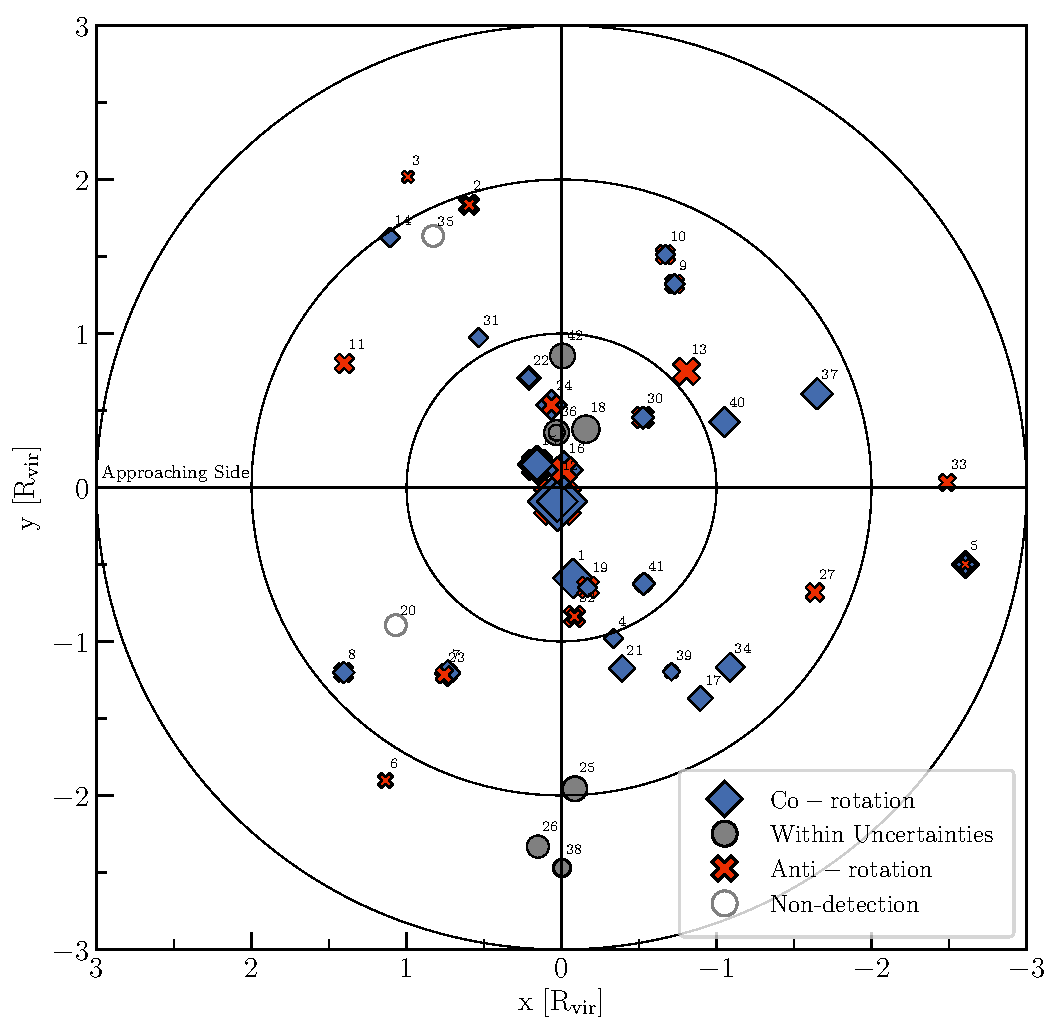
\includegraphics[width=0.96\linewidth]{SALTmap_velstrict_False_non_True_Lstar_0-100_minsep_False_inclim_0.pdf}
        \caption{\small{A map of the locations of each absorber normalized with respect to the galaxy virial radius, with \emph{no} additional constraints. The color and style of each point indicates the line-of-sight velocity compared to that of the rotation of the nearby galaxy. Blue diamonds indicate co-rotation, red crosses indicate anti-rotation, and grey circles indicate cases where either is possible due to a combination of orientation and velocity uncertainties. The size of each point is scaled to reflect the EW of the absorber. Concentric rings indicate distances of 1, 2, and 3 $R_{\rm vir}$. All galaxies are rotated to PA = $90^{\circ}$ or $270^{\circ}$, such that their major axis' are horizontal and their approaching side is on the left as indicated. The number identifiers correspond to the system number given in column (1) of Table \ref{model}.}}
%        \vspace{-5pt}
        \label{full_map}
%        \vspace{-5pt}
\end{figure*}

\begin{figure*}[ht]
\centering
  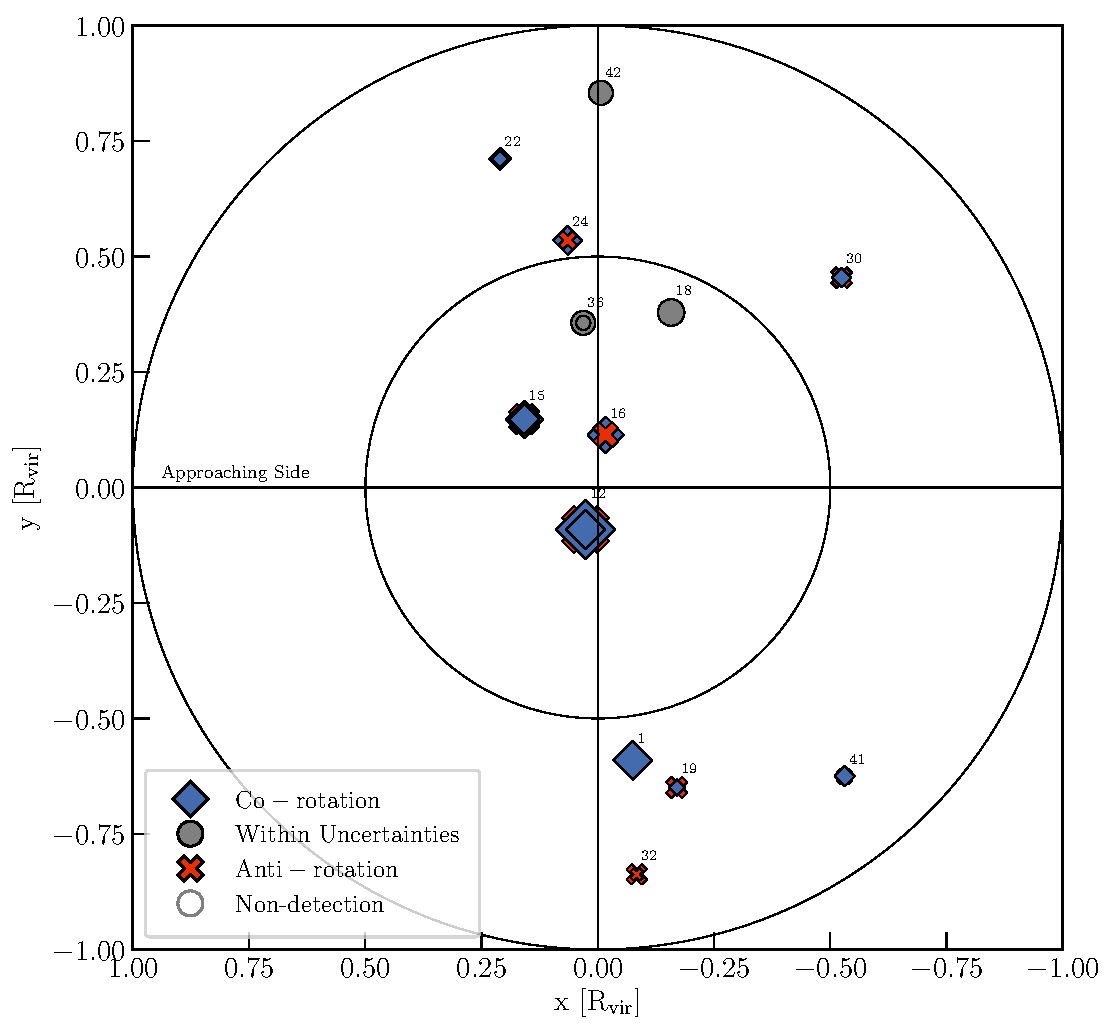
\includegraphics[width=0.96\linewidth]{SALTmap_velstrict_False_non_True_Lstar_0-100_minsep_False_zoom_1_inclim_0.pdf}
  \caption{\small{A map of the locations of each absorber normalized with respect to the galaxy virial radius. A zoom in showing only those systems within $1 R_{\rm vir}$ (exactly the same as Figure \ref{full_map} within $1 R_{\rm vir}$). The color and style of each point indicates the line-of-sight velocity compared to that of the rotation of the nearby galaxy. Blue diamonds indicate co-rotation, red crosses indicate anti-rotation, and grey circles indicate cases where either is possible due to a combination of orientation and velocity uncertainties. The size of each point is scaled to reflect the EW of the absorber. All galaxies are rotated to PA = $90^{\circ}$ or $270^{\circ}$, such that their major axis' are horizontal and their approaching side is on the left as indicated. The number identifiers correspond to the system number given in column (1) of Table \ref{model}.}}
%\vspace{0pt}
\label{zoom_map}
\vspace{2pt}
\end{figure*}



\subsection{Co-rotation Fraction}
Here we consider in aggregate our sample of Ly$\alpha$ absorbers, and the fraction consistent with co-rotation under various cuts and constraints. 

To start we consider the fraction of absorbers which appear to be rotating in the same sense as the nearby galaxy. With no cuts of any kind, we find 52\% of absorbers have velocities consistent with co-rotation with the nearby galaxy based on apparent velocity only. Figure \ref{full_map} presents an map of the locations of each absorber relative to it's assumed host galaxy. In this figure we have rotated every system such that the galaxy major axes are horizontal with the approaching side on the left. Blue-diamonds indicate the absorber has the appropriate velocity sign for co-rotation, red-crosses indicate an anti-alignment, grey circles indicate uncertain systems due to their high azimuth angles, and open grey circles indicate non-detections. We have also scaled the size of each marker according to it's relative EW, and annotated each with a number corresponding to the appropriate system number given in Column (1) of Table \ref{models}. Figure \ref{zoom_map} shows the same map zoomed in to a radius of $1 R_{\rm vir}$.


\begin{figure*}[ht!]
\centering
 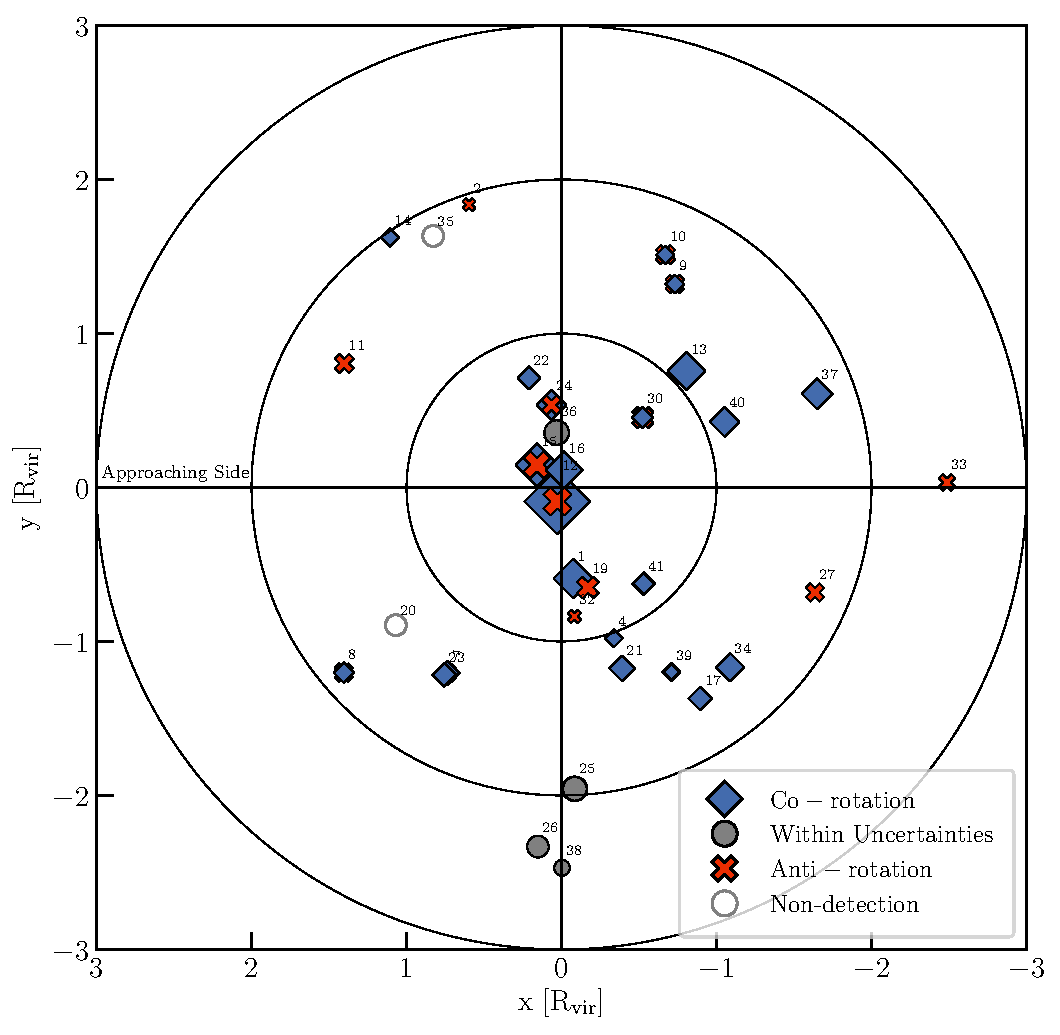
\includegraphics[width=0.49\linewidth]{SALTmap_NFW_model_velstrict_True_non_True_Lstar_0-100_minsep_False_inclim_0.pdf}\label{nfw_map}
  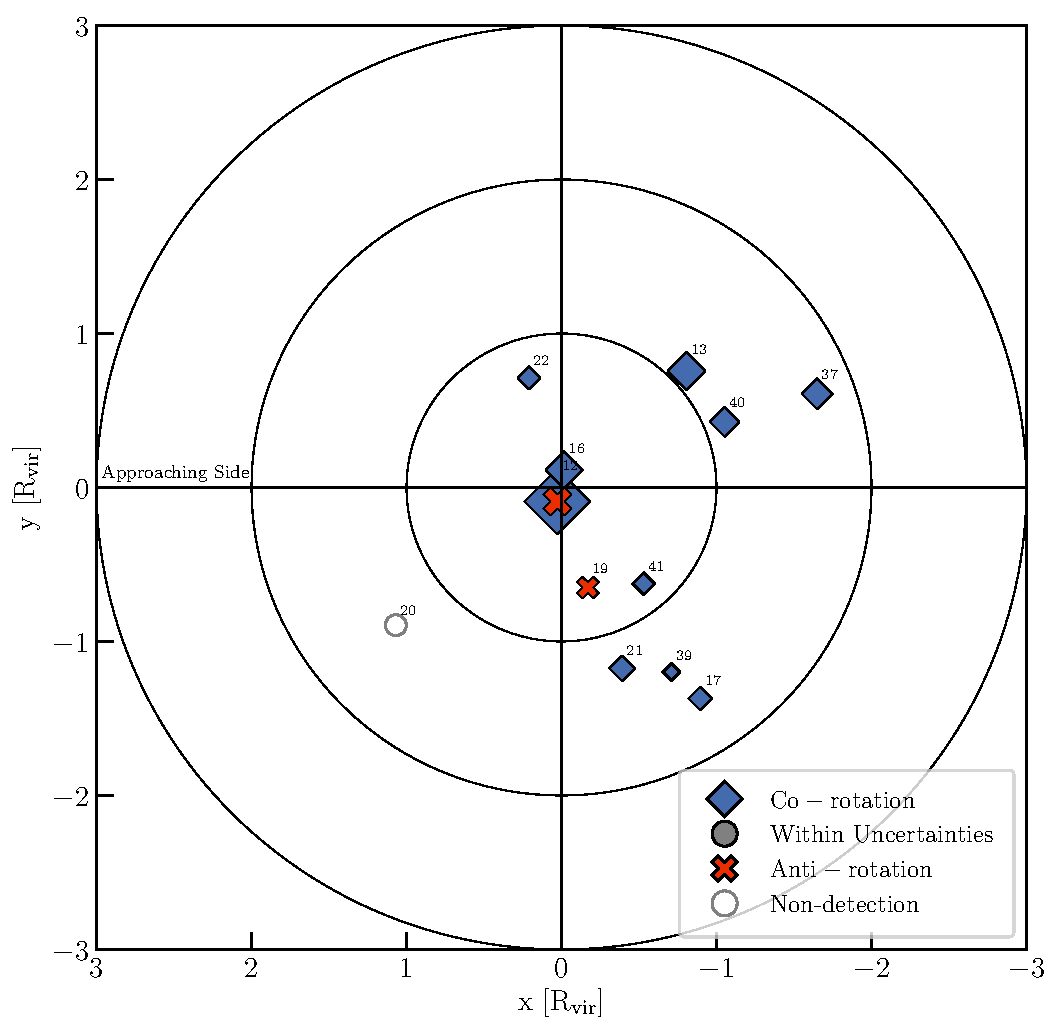
\includegraphics[width=0.49\linewidth]{SALTmap_NFW_model_velstrict_True_non_True_Lstar_0-06_minsep_False_inclim_0.pdf}\label{nfw_lstar_map}
  \caption{\small{Maps of the locations of each absorber normalized with respect to the galaxy virial radius. The color and style of each point indicates the NFW rotation model results for each absorber with a $v_{\rm Ly\alpha} \leq v_{\rm rot}$ constraint imposed. The \textbf{\textit{right}} panel includes only those absorbers near \Lstar $\leq 0.6$ galaxies. Concentric rings indicate distances of 1, 2, and 3 $R_{vir}$. Blue diamonds indicate co-rotation, red crosses indicate anti-rotation, and grey circles indicate cases where either is possible due to a combination of orientation and velocity uncertainties. The size of each point is scaled to reflect the EW of the absorber. All galaxies are rotated to PA = $90^{\circ}$ or $270^{\circ}$, such that their major axis' are horizontal and their approaching side is on the left as indicated. The number identifiers correspond to the system number given in column (1) of Table \ref{model}.}}
  \vspace{10pt}
%\vspace{5pt}
\end{figure*}


%\begin{figure*}[ht!]
%\centering
%  \subfigure[]{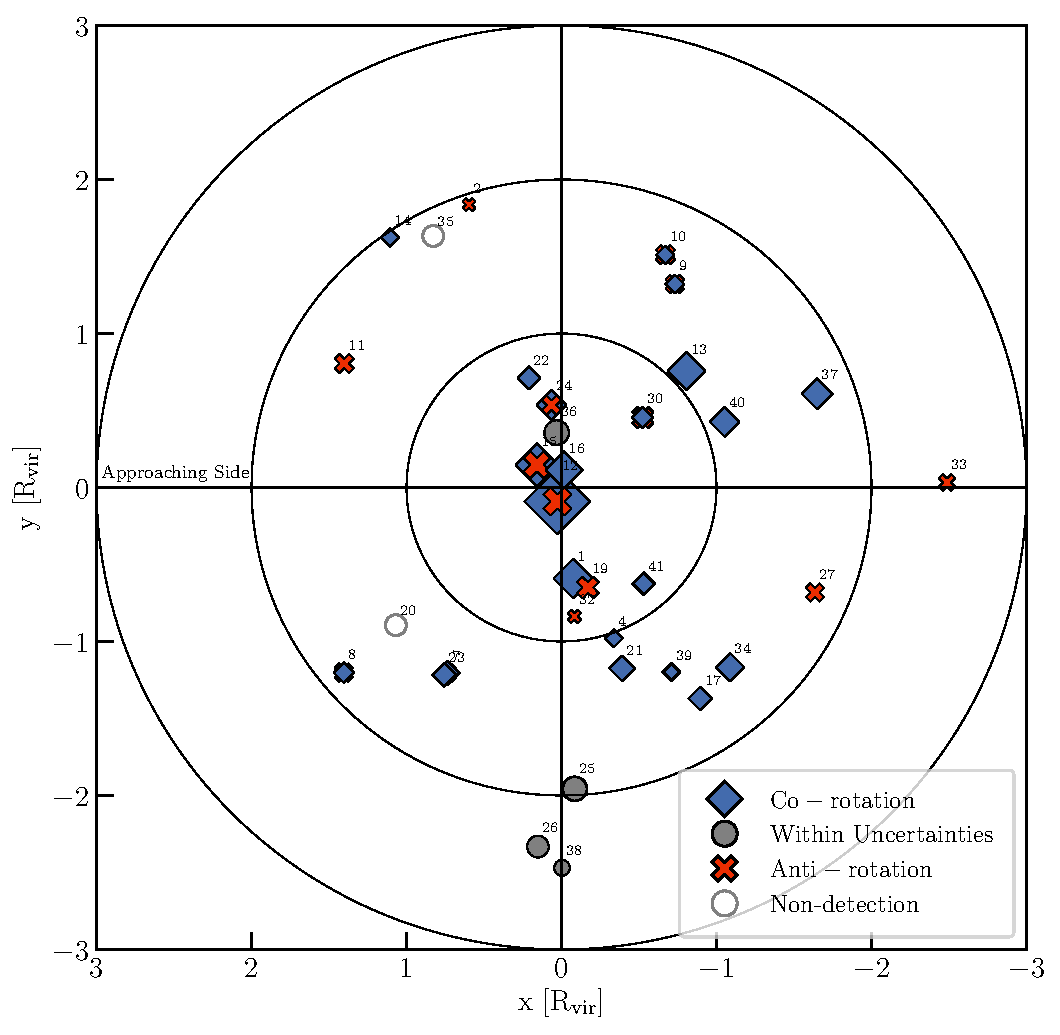
\includegraphics[width=0.4\linewidth]{SALTmap_NFW_model_velstrict_True_non_True_Lstar_0-100_minsep_False_inclim_0.pdf}}\label{nfw_map}
%  \subfigure[]{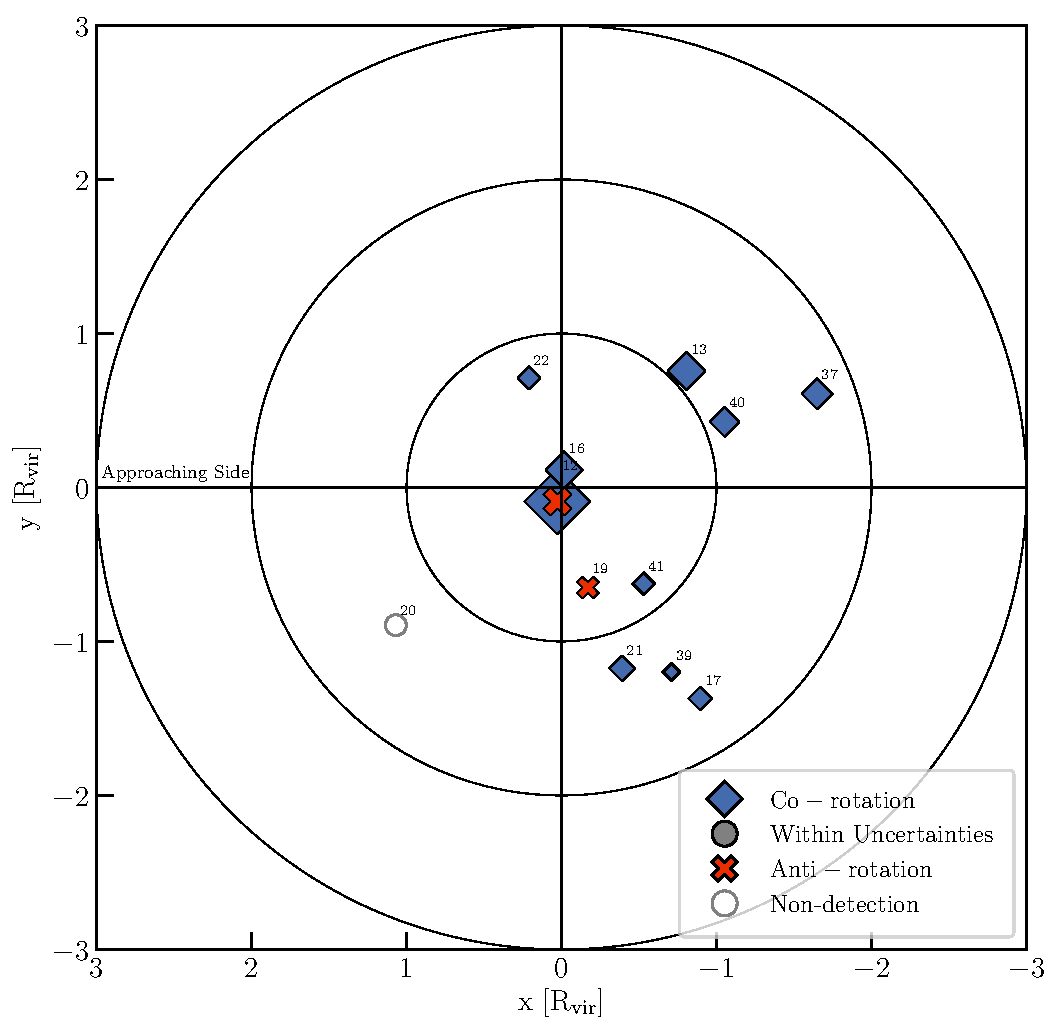
\includegraphics[width=0.4\linewidth]{SALTmap_NFW_model_velstrict_True_non_True_Lstar_0-06_minsep_False_inclim_0.pdf}}\label{nfw_lstar_map}
%  \caption{\small{Maps of the locations of each absorber normalized with respect to the galaxy virial radius. The color and style of each point indicates the NFW rotation model results for each absorber with a $v_{\rm Ly\alpha} \leq v_{\rm rot}$ constraint imposed. Concentric rings indicate distances of 1, 2, and 3 $R_{vir}$. Blue diamonds indicate co-rotation, red crosses indicate anti-rotation, and grey circles indicate cases where either is possible due to a combination of orientation and velocity uncertainties. The size of each point is scaled to reflect the EW of the absorber. All galaxies are rotated to PA = $90^{\circ}$ or $270^{\circ}$, such that their major axis' are horizontal and their approaching side is on the left as indicated. The number identifiers correspond to the system number given in column (1) of Table \ref{model}. \textbf{b)} Same, but here only showing those absorbers near \Lstar $\leq 0.6$ galaxies.}}
%%\vspace{5pt}
%\end{figure*}

%\begin{figure}[ht!]
%        \centering
%        \vspace{0pt}
%        \includegraphics[width=0.5\textwidth]{SALTmap_velstrict_False_non_True_Lstar_0-100_minsep_False_zoom_10_inclim_00.pdf}
%        \caption{\small{A map of the locations of each absorber normalized with respect to the galaxy virial radius, showing only those systems within $1 R_{\rm vir}$. The color and style of each point indicates the line-of-sight velocity compared to that of the rotation of the nearby galaxy. Blue diamonds indicate co-rotation, red crosses indicate anti-rotation, and grey circles indicate cases where either is possible due to a combination of orientation and velocity uncertainties. The size of each point is scaled to reflect the EW of the absorber. Concentric rings indicate distances of 0.5 and 1 $R_{vir}$. All galaxies are rotated to PA = 90 or 270, such that their major axis' are horizontal and their approaching side is on the left as indicated. The number identifiers correspond to the system number given in column (1) of Table \ref{model}.}}
%        \vspace{-5pt}
%        \label{zoom_map}
%\end{figure}
%\begin{figure}[ht!]
%        \centering
%        \vspace{0pt}
%        \includegraphics[width=0.48\textwidth]{SALTmap_NFW_model_velstrict_True_non_True_Lstar_0-100_minsep_False_inclim_00.pdf}
%        \caption{\small{A map of the locations of each absorber normalized with respect to the galaxy virial radius. The color and style of each point indicates the NFW rotation model results for each absorber with a $v_{\rm Ly\alpha} \leq v_{\rm rot}$ constraint imposed. Blue diamonds indicate co-rotation, red crosses indicate anti-rotation, and grey circles indicate cases where either is possible due to a combination of orientation and velocity uncertainties. The size of each point is scaled to reflect the EW of the absorber. Concentric rings indicate distances of 1, 2, and 3 $R_{vir}$. All galaxies are rotated to PA = 90 or 270, such that their major axis' are horizontal and their approaching side is on the left as indicated. The number identifiers correspond to the system number given in column (1) of Table \ref{model}.}}
%%        \vspace{-5pt}
%        \label{nfw_map}
%\end{figure}



A cursory look at Figures \ref{full_map} and \ref{zoom_map} reveals several interesting results. First, the highest EW absorbers are all found within $1 R_{\rm vir}$. This is not surprising, given the results by numerous groups claiming an impact parameter - equivalent width anti-correlation (see e.g., \citealt{french2017}, and references therein). Second, many of our absorbers, and many co-rotating ones, lie in the $1 - 2 R_{\rm vir}$ region. Previously, most groups have concentrated on studying the sub-$1 R_{\rm vir}$ regime, but doing so clearly does not reveal the whole physical picture. Third, just over half ($52\%$) of galaxy-QSO systems reveal multiple distinct velocity components, and they tend to be oriented such that one component is co- and one anti-rotating with the nearby galaxy.


\begin{figure*}[ht!]
\centering
  \subfigure[]{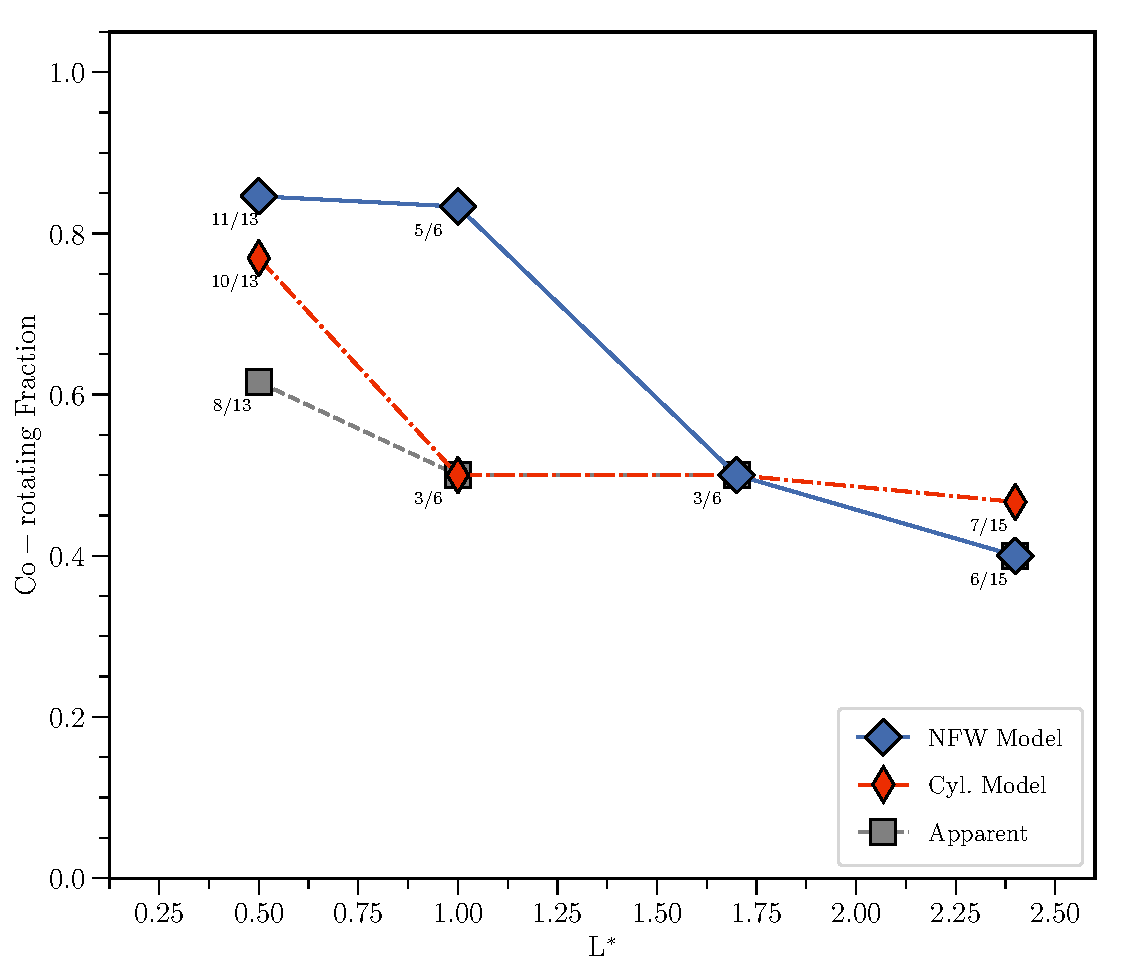
\includegraphics[width=0.48\linewidth]{SALT_corotate_vs_Lstar_velstrict_True_non_True_Lstar_06_minsep_False_ALLmodel.pdf}}\label{Lstar_fraction}
  \subfigure[]{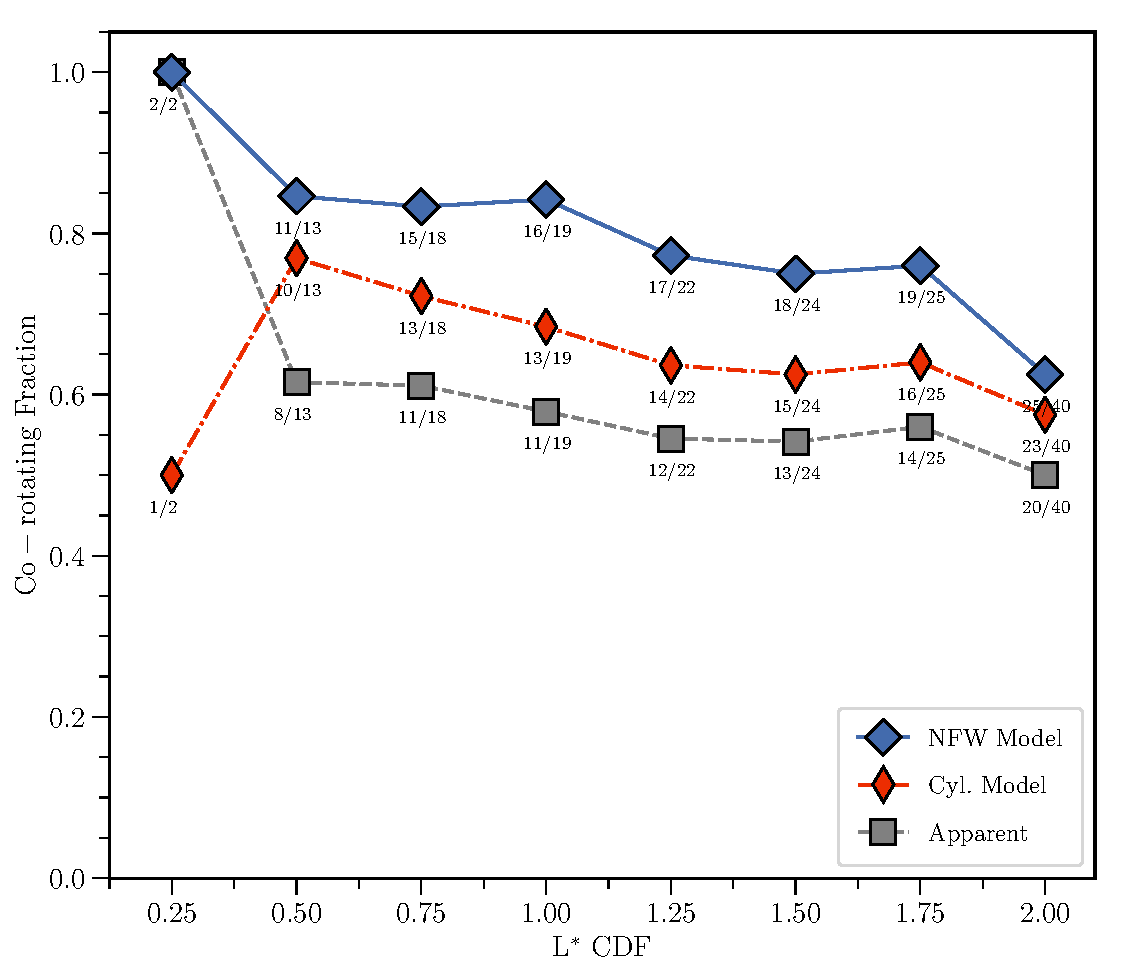
\includegraphics[width=0.48\linewidth]{SALT_corotate_vs_Lstar_minimum_velstrict_True_non_True_Lstar_06_minsep_False_ALLmodel.pdf}\label{Lstar_fraction_cdf}}
  \caption{\small{\textbf{Top:} The fraction of co-rotating absorbers as a function of \Lstar. The upper edges of the \Lstar~ bins are located at 0.5, 1.0, 1.7, and $>1.7$ \Lstar~ (i.e., all systems $1.7 $\Lstar~ and higher). \textbf{Bottom:} The fraction of co-rotating absorbers as a function of cumulative \Lstar~ distribution. All systems are included at the \Lstar$=2.0$ bin (this bin includes galaxies brighter than 2.0\Lstar~ as well), then only galaxies with \Lstar~ $ \leq 1.8$ are included at \Lstar~$ =1.8$, and so on.}}
\vspace{10pt}
\label{Lstar_fraction}
\end{figure*}

However, a more in-depth look at the underlying data reveals that many of these absorbers have $\Delta v$ much larger than the inclination-corrected galaxy rotation velocity ($v_{\rm rot}$). In other words, the velocity of the absorber relative to galaxy systemic is much greater than the rotation velocity of the galaxy disk. This results in a much smaller fraction of co-rotating absorbers when compared to our cylindrical and NFW profile models (41\% and 45\%, respectively), which will never output a velocity higher than $v_{\rm rot}$. In undertaking this study we necessarily must begin by assuming that absorption within some velocity limit and impact parameter from a galaxy is likely associated with that galaxy. To start with we set these limits at $\Delta v_{\rm max} = 400$ \kms~and $\rho_{\rm max} = 3 R_{\rm vir}$. 

Let us now instead consider only absorbers with $|\Delta v| \leq v_{\rm rot}$ \kms, or absorbers with velocities differences no greater than the maximal galaxy rotation velocity (in other words the we are only considering absorbers where $|v_{\rm Ly\alpha} - v_{\rm sys}| \leq v_{\rm rot}$ \kms~, which are those absorbers within the velocity range of $\pm$ rotation $-$ this constraint removes 22 from our original sample of 65 absorbers). This constraint thus focuses only on absorbers whose velocity falls within the range of possible rotation-related velocities. While this could be interpreted as a bias in the sample, we are really only setting the $\Delta v$ velocity separation limit on a case-by case basis instead of globally given the additional information available to us. We could just as easily have started this study by looking for only absorbers within $\Delta v = 150$ \kms~of a galaxy instead of $\Delta v = 400$ \kms, which would have a similar overall effect. This criteria instead narrows the focus to only those absorbers kinematically close enough to a galaxy to test for a co-rotation fraction with minimal contamination from $\rm Ly\alpha$ forest lines.




%\begin{figure}[ht!]
%        \centering
%        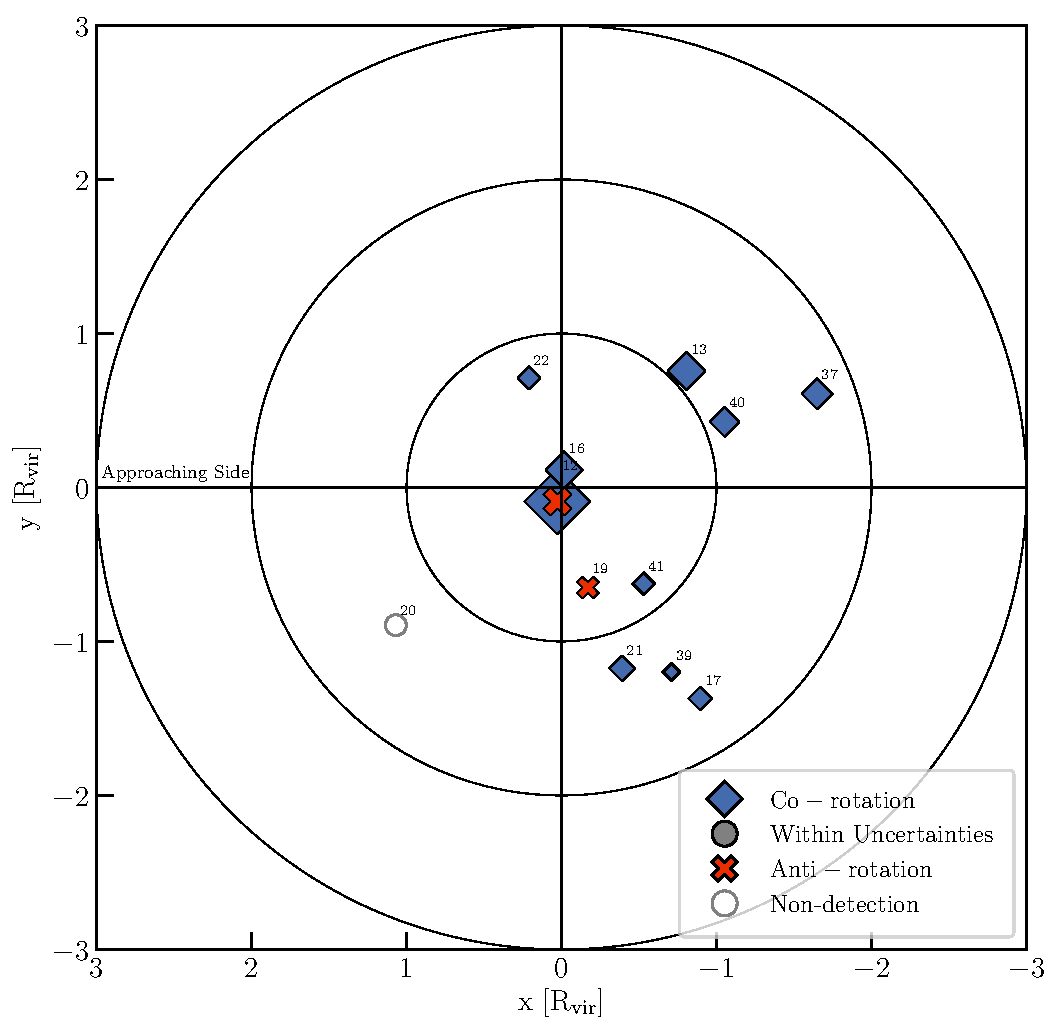
\includegraphics[width=0.98\linewidth]{SALTmap_NFW_model_velstrict_True_non_True_Lstar_0-06_minsep_False_inclim_0.pdf}
%        \caption{\small{A map of the locations of each absorber normalized with respect to the galaxy virial radius. The color and style of each point indicates the NFW rotation model results for each absorber with $\Delta v \leq v_{rot}$ and \Lstar $\leq 0.6$ constraints imposed. Blue diamonds indicate co-rotation, red crosses indicate anti-rotation, and grey circles indicate cases where either is possible due to a combination of orientation and velocity uncertainties. The size of each point is scaled to reflect the EW of the absorber. Concentric rings indicate distances of 1, 2, and 3 $R_{vir}$. All galaxies are rotated to PA = $90^{\circ}$ or $270^{\circ}$, such that their major axis' are horizontal and their approaching side is on the left as indicated. The number identifiers correspond to the system number given in column (1) of Table \ref{model}.}}
%\end{figure}



%\begin{figure}[ht!]
%\centering
%  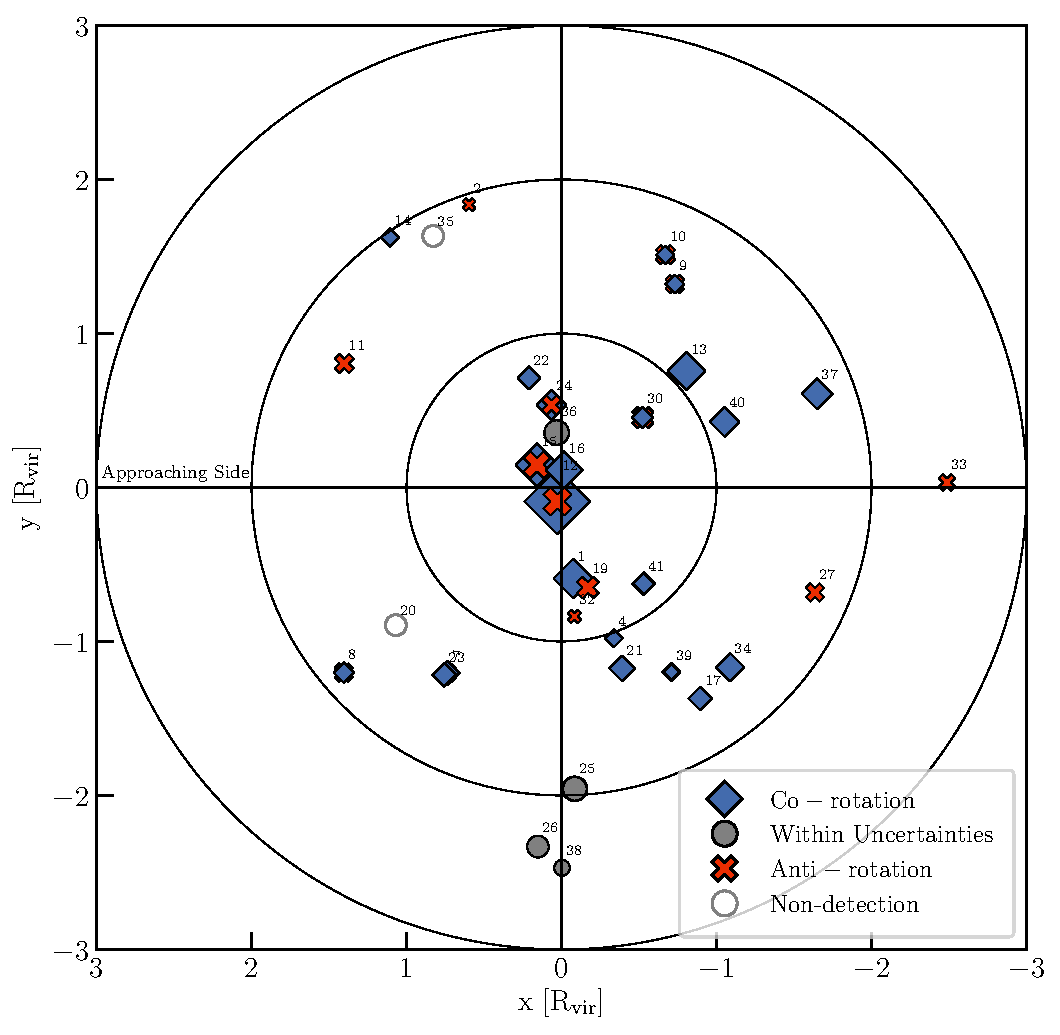
\includegraphics[width=0.96\linewidth]{SALTmap_NFW_model_velstrict_True_non_True_Lstar_0-100_minsep_False_inclim_0.pdf}
%  \caption{\small{A map of the locations of each absorber normalized with respect to the galaxy virial radius. The color and style of each point indicates the NFW rotation model results for each absorber with a $v_{\rm Ly\alpha} \leq v_{\rm rot}$ constraint imposed. Concentric rings indicate distances of 1, 2, and 3 $R_{vir}$. Blue diamonds indicate co-rotation, red crosses indicate anti-rotation, and grey circles indicate cases where either is possible due to a combination of orientation and velocity uncertainties. The size of each point is scaled to reflect the EW of the absorber. All galaxies are rotated to PA = $90^{\circ}$ or $270^{\circ}$, such that their major axis' are horizontal and their approaching side is on the left as indicated. The number identifiers correspond to the system number given in column (1) of Table \ref{model}.}}
%%\vspace{5pt}
%\label{nfw_map}
%\end{figure}
%\begin{figure}[ht!]
%        \centering
%        \vspace{0pt}
%        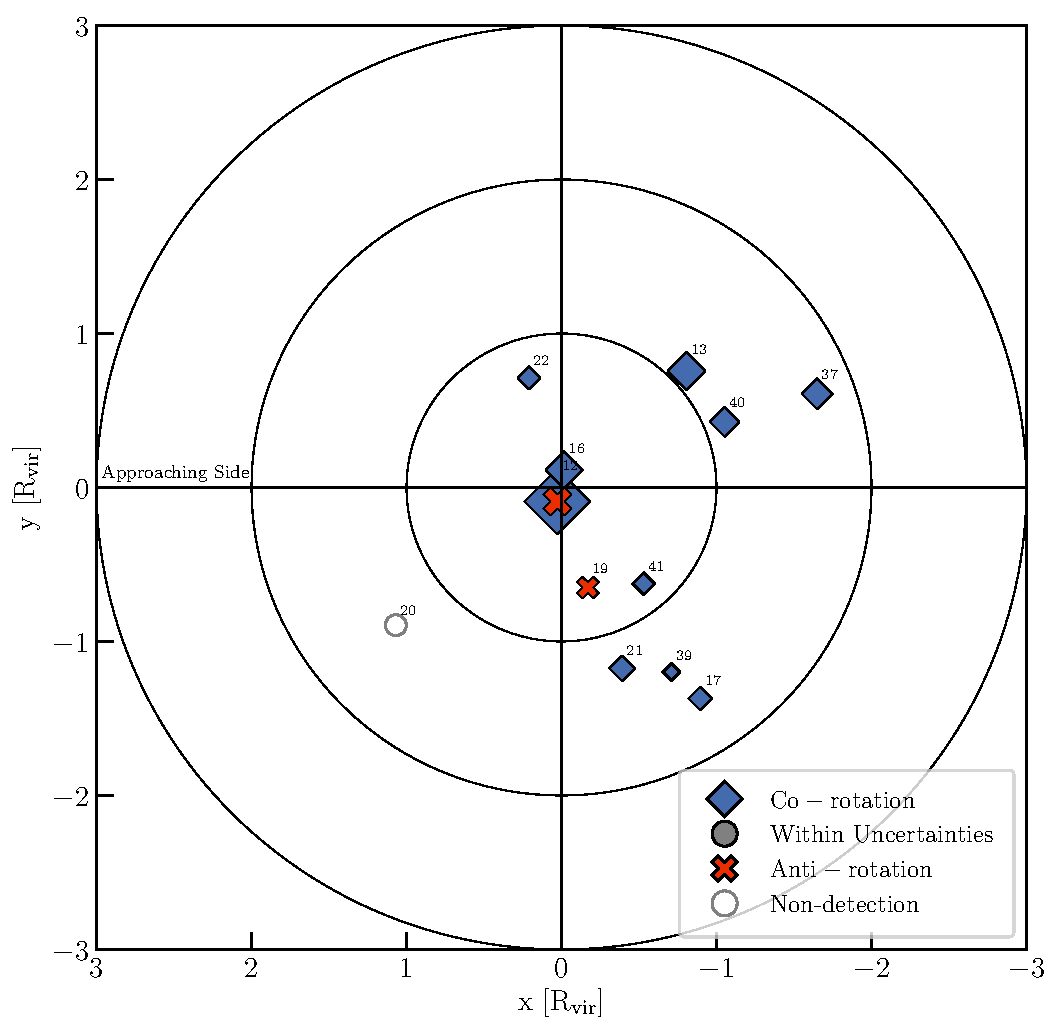
\includegraphics[width=0.98\linewidth]{SALTmap_NFW_model_velstrict_True_non_True_Lstar_0-06_minsep_False_inclim_0.pdf}
%        \caption{\small{A map of the locations of each absorber normalized with respect to the galaxy virial radius. The color and style of each point indicates the NFW rotation model results for each absorber with $\Delta v \leq v_{rot}$ and \Lstar $\leq 0.6$ constraints imposed. Blue diamonds indicate co-rotation, red crosses indicate anti-rotation, and grey circles indicate cases where either is possible due to a combination of orientation and velocity uncertainties. The size of each point is scaled to reflect the EW of the absorber. Concentric rings indicate distances of 1, 2, and 3 $R_{vir}$. All galaxies are rotated to PA = $90^{\circ}$ or $270^{\circ}$, such that their major axis' are horizontal and their approaching side is on the left as indicated. The number identifiers correspond to the system number given in column (1) of Table \ref{model}.}}
%        \vspace{5pt}
%        \label{nfw_lstar_map}
%\end{figure}


With this rotation-based velocity constraint in place the co-rotating fractions for our cylindrical and NFW models increase to 58\% and 63\%, while the apparent co-rotation fraction decreases slightly to 50\%. Consistently, we find our cylindrical model to predict an $\sim 8-10 \%$ higher co-rotation fraction than the straight apparent velocity analysis yields, and our NFW model tends to predict an additional $\sim 5\%$ increase. This is a not wholly unexpected, and yet refreshing result; simulations have predicted that galaxies are strongly linked to their surroundings and share angular momentum, which should result in a higher than $50\%$ halo-gas co-rotation fraction. However, the simple apparent on-sky velocity method ignores the complexities of sampling a 3-dimensional structure with a 1-dimensional QSO sightline. It appears then that the NFW model, the most physically motivated of the three, systematically recovers a higher fraction of this co-rotating gas. For brevity's sake we will concentrate only on the NFW model results from here onwards. Figure \ref{nfw_map} shows another absorber location map, this time colored according to our NFW model results.


%One additional constraining step we consider is to only include galaxies which have no neighbors within at least 20 kpc. The disruptions caused by near neighbors to both galaxy \HI~disks and halos has been well established observationally, so a 20 kpc minimum separation should at least remove the systems most likely to be disrupted. This constraint alone leads to a co-rotating fraction of 50\%. Combining both constraints (i.e. $\Delta v \leq \lvert v_{\rm rot} \rvert $ and $\rho \ge 20$ kpc nearest neighbor) results in a 62\% co-rotating fraction.

%\footnote{From here on we concentrate on the results using our NFW profile model. The cylindrical model results do not differ in a systematically interesting way.}



\subsection{Co-rotation as a function of \Lstar}
%Next, we consider the effect of galaxy luminosity. We separate our sample around $0.6$\Lstar,  while keeping our $\Delta v \leq v_{\rm rot} \pm 10$ \kms~constraint and relaxing the 20 kpc nearest-neighbor criteria in order to maximize the sample size. 

Next, we consider the effect of galaxy luminosity. We separate our sample around $0.6$\Lstar,  while keeping our $|\Delta v| \leq v_{\rm rot}$ \kms~constraint in place. This results in 15 absorbers near $L \leq 0.6$\Lstar~galaxies and 30 around more luminous galaxies. The co-rotating fraction around luminous galaxies is then 48\%, compared to 87\% around $L \leq 0.6$\Lstar~ galaxies. Figure \ref{nfw_lstar_map} shows an absorber map for these $L \leq 0.6$\Lstar~ galaxies only. 

Furthermore, we find this co-rotation fraction smoothly decreases as a function of \Lstar, as shown in Figure \ref{Lstar_fraction}(a). In this figure we have binned galaxy-absorber systems into the following 4 ranges: $L/$\Lstar $= [0-0.5],~(0.5-1.0],~(1.0-1.7],$ and $(1.7-\infty)$. This uneven bin spacing was chosen to produce as evenly occupied bins as possible, and does not affect the overall trend. Unfortunately there are a large number of systems between $1.7-1.8$ \Lstar, so no splitting exists to produce perfectly even bins. The co-rotation fraction is labeled explicitly underneath each data point for clarity.

In Figure \ref{Lstar_fraction_cdf} we consider the co-rotation fraction as a function of the cumulative \Lstar~ distribution (i.e., every consecutive \Lstar~ bin includes all previous bins' data as well). Here, bins are evenly distributed in $0.25$\Lstar~ increments with the final bin containing all systems. Thus, nearly $90\%$ of absorbers near \Lstar~ or fainter galaxies are co-rotating based on our NFW model results, but this fraction decreases to $\sim 80\%$ for $1.5$\Lstar~ or fainter galaxies, and to $63\%$ for all galaxies. As seen in Figure \ref{Lstar_fraction_cdf}, this trend is also model independent; it appears nearly identically but offset downward in both the cylindrical model (red-rhombus) and apparent velocity only (grey-square) samples.

%As seen in red rhombus and grey square markers in Figure \ref{Lstar_fraction_cdf}, this trend appears identically but offset downward in both the cylindrical model and apparent velocity only samples.



Given recent simulation results suggesting that co-rotating accretion gas is predominately cold-mode for low-mass galaxies in the local Universe, this may be a signature of this co-rotating, cold-mode accreting gas. Additionally, \cite{lutz2018} find that galaxies with high \HI mass compared to their stellar mass have higher halo angular momentum, which may be impeding their ability to efficiently form stars. While we do not have independent measures of \HI and stellar mass for our galaxies, it may not be unreasonable to think that these high angular momentum galaxies reside toward the lower luminosity end of our sample.

\subsection{Doppler $b$-parameters}
Finally, we consider the Doppler $b$-parameters of our absorber sample. Figure \ref{b_hist} shows the distribution of $b$-parameters for all velocity-constrained Ly$\alpha$ absorbers ($|\Delta v| \leq v_{\rm rot}$ \kms). In the top panel of Figure \ref{b_hist} we separate them into co-rotating and anti-rotating subsets, in the middle panel we do the same but only for $\rho \leq 1 R_{\rm vir}$, and on the bottom we separate based on absorbers near \Lstar $\leq 0.6$ and \Lstar $ > 0.6$ galaxies. Interestingly, we find that \emph{lower} $b$-parameter absorbers tend to be both anti-rotating and found near \Lstar $> 0.6$ galaxies. As previously discussed however, the picture described by the simulations of \cite{stewart2011b} and others describes a scenario where co-rotating gas is predominately the product of cold-mode accretion. Hotter, outflowing gas would likely carry angular momentum from the disk with it, but this would be quickly lost as the outflows expand into the halo and result in negligible observable rotation signature. 

In Figure \ref{b_vs_dv2}(b) we show how the $b$-parameters vary as a function of $\Delta v$ for co-rotating versus anti-rotating absorbers. We would expect the co-rotating sample to occupy a narrower $\Delta v$ space based on their definition ($\Delta v$ fitting within the velocity bounds given by our NFW model), but the elevated $b$-parameters for these compared to the relatively flat distribution for anti-rotators is intriguing. Aside from a single $\rm Ly\alpha$ line toward SDSSJ104335.90+115129.0 and NGC3351, all the anti-rotators have $b \lesssim 50$ \kms. As these are higher than expected for purely thermal motions within a single $\rm Ly\alpha$ structure, we may be observing either a number of clouds that are close in velocity space or a filament with a range of turbulent, internal velocities. In this scenario these high $b$-parameters would be consistent with filamentary inflows versus around higher \Lstar~ galaxies where virial shocks are perhaps breaking larger structures into smaller, more isolated cloudlets and producing lower $b$-parameter absorption.


\begin{figure}[ht!]
\centering
  \subfigure[]{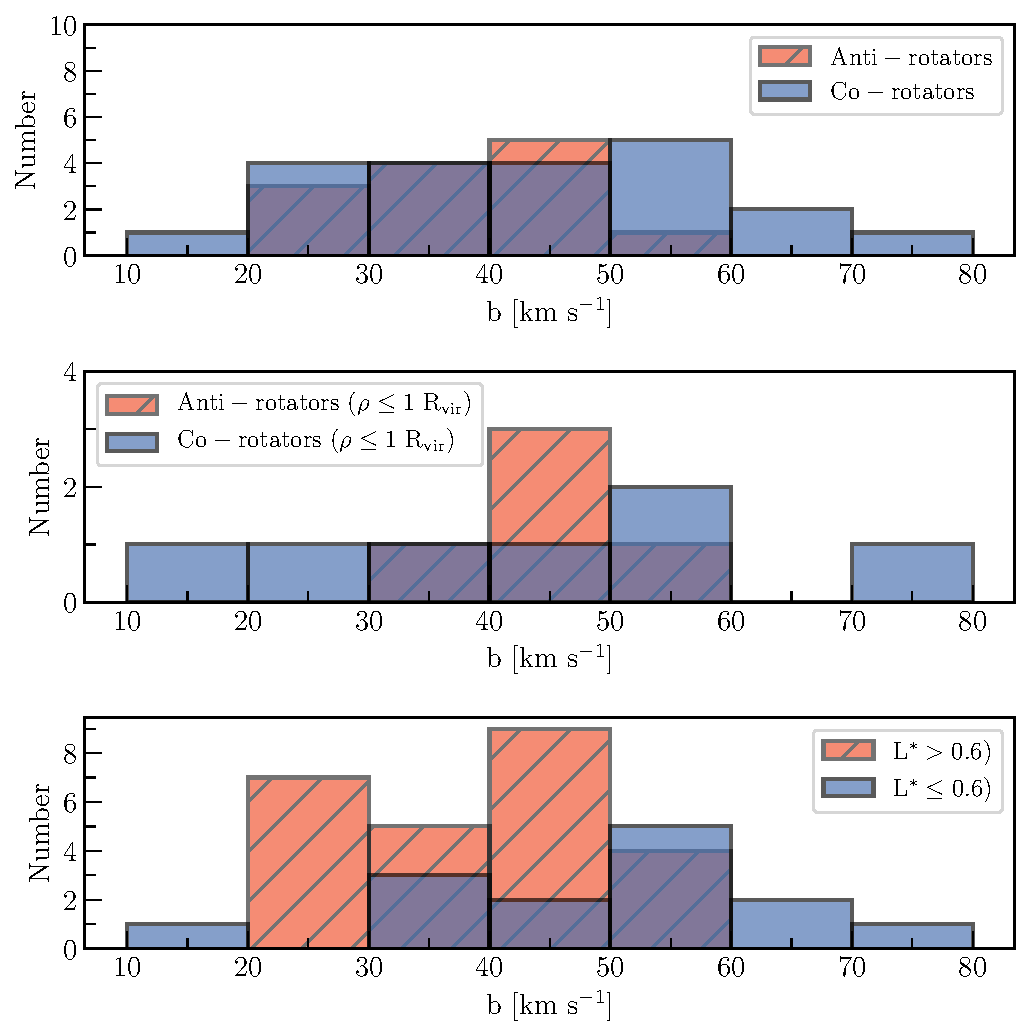
\includegraphics[width=0.946\linewidth]{SALT_bhist_NFW_velstrict_True_non_True_Lstar_06_minsep_False_fits_True.pdf}\label{b_hist}}
  \subfigure[]{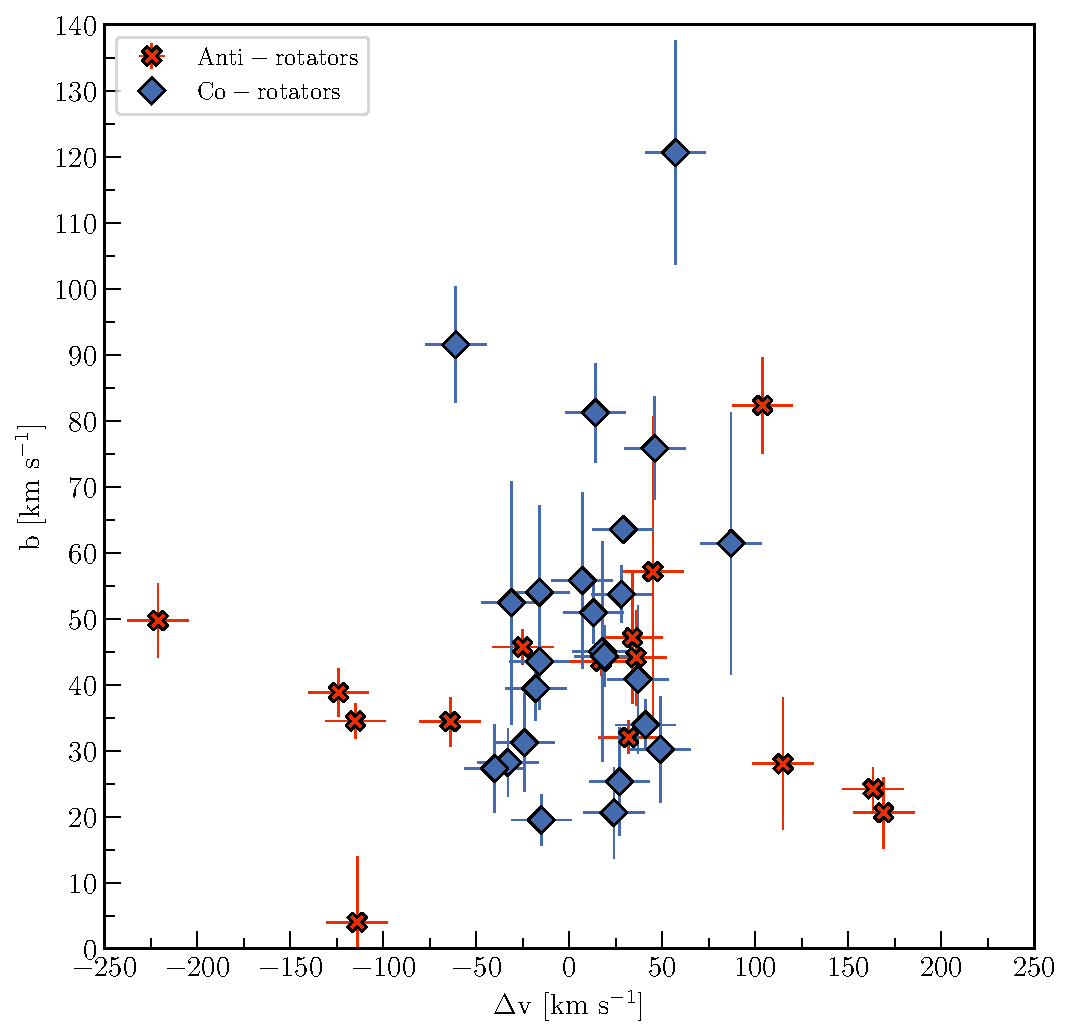
\includegraphics[width=0.946\linewidth]{SALT_b_vs_dv_NFW_velstrict_True_non_True_Lstar_06_minsep_False_fits_True.pdf}}\label{b_vs_dv2}
  \caption{\small{\textbf{Top:} The distributions of Doppler $b$-parameters for all Ly$\alpha$ absorbers with $\Delta v \leq v_{\rm rot} \pm 10$ \kms. The co-rotating versus anti-rotating designation here is based on NFW results. In the middle we do the same but only for $\rho \leq 1 R_{vir}$, and on the bottom we separate based on absorbers near \Lstar $\leq 0.6$ (blue) and \Lstar $ > 0.6$ (red-hatched) galaxies.  \textbf{Bottom:} The Doppler $b$-parameters of each absorber as a function of $\Delta v$, split into co-rotating (blue diamonds) and anti-rotating (red crosses). The data point for the NGC3067-3C232 LLS ($b = 245.2 \pm 25.9,  ~\Delta v = -68.0 \pm 11$ \kms, co-rotating) is not shown in order to highlight the majority distribution in greater detail.}}
\label{b_vs_dv2}
\end{figure}


\begin{deluxetable*}{l | c c c | c c | c c}
\tabletypesize{\footnotesize}
\tablewidth{0pt}
\tablecaption{CGM Rotation: Summary of Results\label{results}}
\tablehead{
\colhead{Sub-sample}  		&  \colhead{Co-rotating} 		&  \colhead{Anti-rotating}		&  \colhead{Uncertain}  	&  \colhead{Co-rotating} 		&  \colhead{Anti-rotating} 		&  \colhead{Co-rotating} 		&  \colhead{Anti-rotating}	\\
			  			&          			 		& 			 			&					& $\rho \leq 1$				& $\rho \leq 1$				& $\rho >$ 1				& $\rho > 1$		}
\startdata
Apparent Vel.				&	29					&	27					&	9				&		12				&		10				&	17					&	17				\\
\hline
Cyl. Model				&	23					&	33					&	9				&		10				&		12				&	13					&	21				\\
\hline
NFW Model				&	25					&	31					&	9				&		10				&		12				&	15					&	19				\\
\hline \\
\hline
NFW w/ Constraint:			&	25					&	15					&	5				&		10				&		7				&	15					&	8				\\
$ \lvert \Delta v \rvert \leq v_{\rm rot}  \pm 10$ \kms		&						&						&					&						&						&						&					\\
\hline
NFW w/ Constraint:			&	12					&	14					&	6				&		2				&		4				&	10					&	10				\\
Nearest $\rho \geq 20$ kpc	&						&						&					&						&						&						&					\\
\hline
NFW w/ Both Constraints		&	12					&	9					&	2				&		2				&		2				&	10					&	7				\\
\hline \\
\hline
NFW w/ $\Delta v$ Constraint:	&	13					&	2					&	0				&		6				&		2				&	7					&	0				\\
$[0 \leq $\Lstar $ \leq 0.6]$		&					&						&					&						&						&						&					\\
\hline
NFW w/ $\Delta v$ Constraint:	&	12					&	13					&	5				&		4				&		5				&	8					&	8				\\
$[$\Lstar $ > 0.6]$				&					&						&					&						&						&						&					\\
\enddata
%\tablecomments{Comments.}
%\vspace{-5pt}
\end{deluxetable*}

\section{Summary} \label{summary}
We have presented complimentary COS Ly$\alpha$ absorption-line and nearby galaxy rotation curve analysis for a sample of 42 galaxy-QSO pairs, resulting in the largest yet sample of its kind. Our main conclusions are the following:
\vspace{10pt}

1. The fraction of Ly$\alpha$ absorbers appearing to co-rotate with the nearby galaxy smoothly declines as a function galaxy luminosity (\Lstar). Our overall co-rotation fraction is consistent with the simulation results of \cite{stewart2011b, stewart2013}, and effect of galaxy luminosity on halo gas co-rotation is consistent with predicted cold-mode filamentary accretion schemes. 

\vspace{10pt}

%The fraction of co-rotating $\rm Ly\alpha$ absorbers smoothly decreases as a function of the luminosity (\Lstar) of the nearby (probable-) host galaxy. 
2. Based on the predicted velocity of the NFW halo model, 87\% of absorbers co-rotate around $\rm \leq 0.6 $\Lstar~ galaxies, which falls to 77\% around $\rm \leq 1.5$ \Lstar~ galaxies, and down to 63\% around all galaxies at $z \sim 0$.

\vspace{10pt}

3. Two thirds of all $\rm Ly\alpha$ absorbers are found with velocity separations less than or equal to the nearby galaxy rotation velocity ($\Delta v \leq \lvert v_{\rm rot} \rvert$ \kms). This includes systems with multiple galaxies and undoubtedly complex velocity fields. Restricting this study to only isolated galaxy-QSO systems would likely result in an even higher fraction.

%Two thirds of all $\rm Ly\alpha$ absorbers within $3 R_{\rm vir}$ and $\Delta v = 400$ \kms~of our galaxies with known kinematics reside within $\pm v{\rm rot}$

%A simple cylindrical halo model An NFW rotation curve fit, which results in a galaxy rotation velocity which approaches systemic 

\vspace{10pt}

4. A simple cylindrical halo model with rotation velocities smoothly declining based on an NFW rotation curve fit results in the highest co-rotation fraction for $\rm Ly\alpha$ absorbers ($63\%$).

\vspace{10pt}

5. Co-rotating absorbers (when chosen from the sample restricted to $\rvert \Delta v\lvert \leq  v_{\rm rot}$ \kms) occupy a wide range in Doppler $b$-parameter, while anti-rotators have mostly $b \leq 50$ \kms. A remarkably similar split is found for absorbers near $L \leq 0.6 $\Lstar~ vs $L > 0.6$\Lstar~ galaxies. This could add further evidence for our proposed cold-mode accretion explanation if these enhanced $b$-parameters are caused by the blending of multiple absorption components close in velocity space within a filament.

\vspace{10pt}


\acknowledgements

D. M. F. thanks Claire Murray for useful insights, particularly related to our halo model, and Julie Davis for invaluable SALT data reduction pointers. This research has made use of the NASA/IPAC Extragalactic Database (NED) which is operated by the Jet Propulsion Laboratory, California Institute of Technology, under contract with the National Aeronautics and Space Administration. Based on observations with the NASA/ESA \textit{Hubble Space Telescope}, obtained at the Space Telescope Science Institute (STScI), which is operated by the Association of Universities for Research in Astronomy, Inc., under NASA contract NAS 5-26555. Spectra were retrieved from the Barbara A. Mikulski Archive for Space Telescopes (MAST) at STScI. Some of the observations reported in this paper were obtained with the Southern African Large Telescope (SALT) under program 2016-1-SCI-062 (PI: Wakker). Over the course of this study, D.M.F. and B.P.W. were supported by grant AST-118913 from the National Science Foundation and GO-14240, GO-14268, and GO-14588 from the Space Telescope Science Institute.

%AST-1108913, awarded by the US National Science Foundation, and by NASA grants \textit{HST}-AR-12842.01-A, \textit{HST}-AR-13893.01-A, and \textit{HST}-GO-14240 (STScI). 

\facility{HST (COS), SALT (RSS)}
\clearpage

%\nocite{*}
%\bibliography{rotation_bib}
%\bibliography{/Users/frenchd/Research/bib}{}
%\bibliography{/Users/clairemurray/Desktop/DMF_thesis/bib}
\bibliography{/Users/frenchd/Research/inclination/git_inclination/thesis_bib}
\bibliographystyle{apj}

\clearpage

\appendix
%\section{Galaxy Sample}
\label{galaxy_sample}

\section{SALT Galaxies} \label{SALT_sample}
In this section we summarize each galaxy-QSO system observed by SALT. We calculate impact parameters to QSOs and galaxy-absorber velocity separations ($\Delta v = v_{\rm Ly\alpha} - v_{\rm sys}$) based on our measured $v_{sys}$ values. Both measured and previously published values for $v_{sys}$ are given in Table \ref{salt_targets} for reference. We provide rotation curves and finder chart images for the sub-sample of galaxies with newly observed SALT data.

\subsection{CGCG039-137}

CGCG039-137 is an isolated Scd type galaxy with a measured systemic velocity $v_{\rm sys} = 6918 \pm 24$ \kms~and inclination of $i = 72^{\circ}$. The QSO RX\_J1121.2+0326 is located nearby at an impact parameter of 99 kpc and azimuth angle of $71^{\circ}$ on the receding side. The data for  RX\_J1121.2+0326 has low signal-to-noise ($\sim 4.2$), but we are able to detect Ly$\alpha$ at 6975 \kms~, which, at $\Delta v = 57$ \kms, lies well within the range of projected velocities consistent with co-rotation (cylindrical model = [-36, 137], NFW = [-37, 164] \kms). 

\begin{figure}[hb]
\centering
%  \subfigure[]{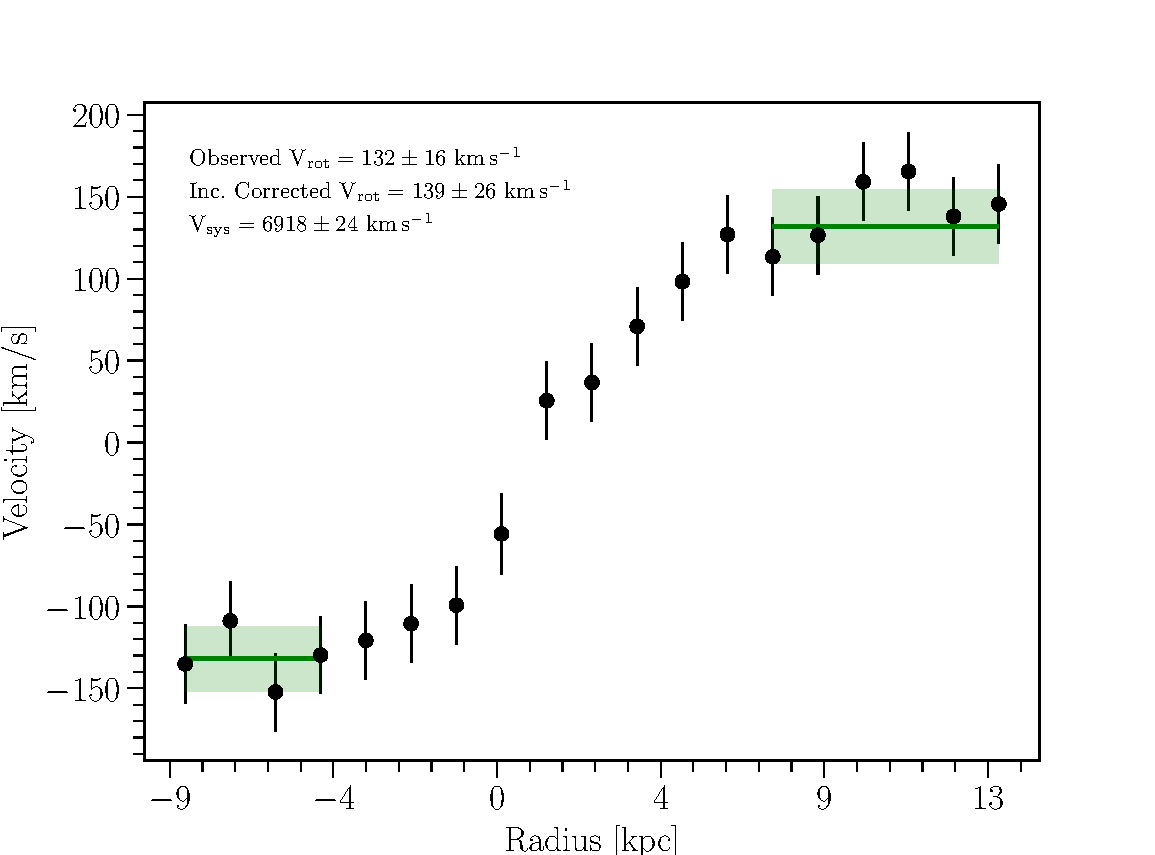
\includegraphics[width=.54\linewidth]{CGCG039-137_2_rotation_curve_xphys_helio_vobs_vrotObs_new4.pdf}}{\label{rotationcurve_CGCG039-137}}
  \subfigure[]{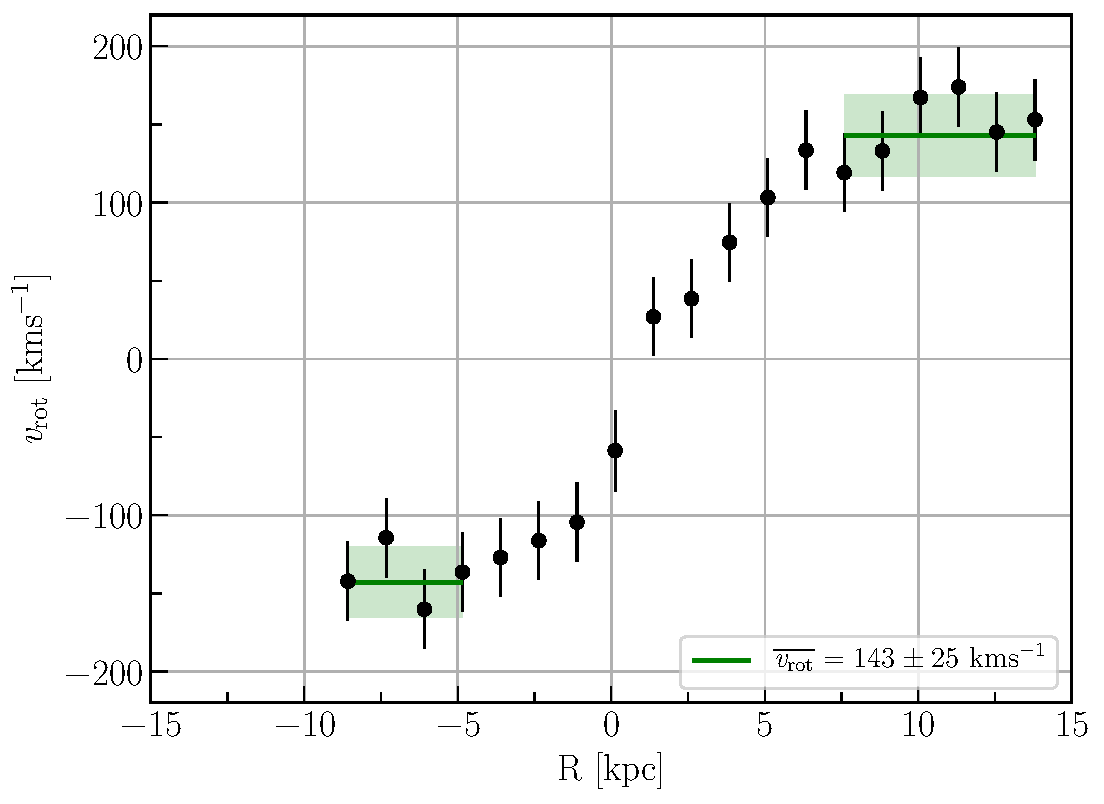
\includegraphics[width=.54\linewidth]{CGCG039-137-rotation_curve_nice3.pdf}}{\label{rotationcurve_CGCG039-137}}
  \subfigure[]{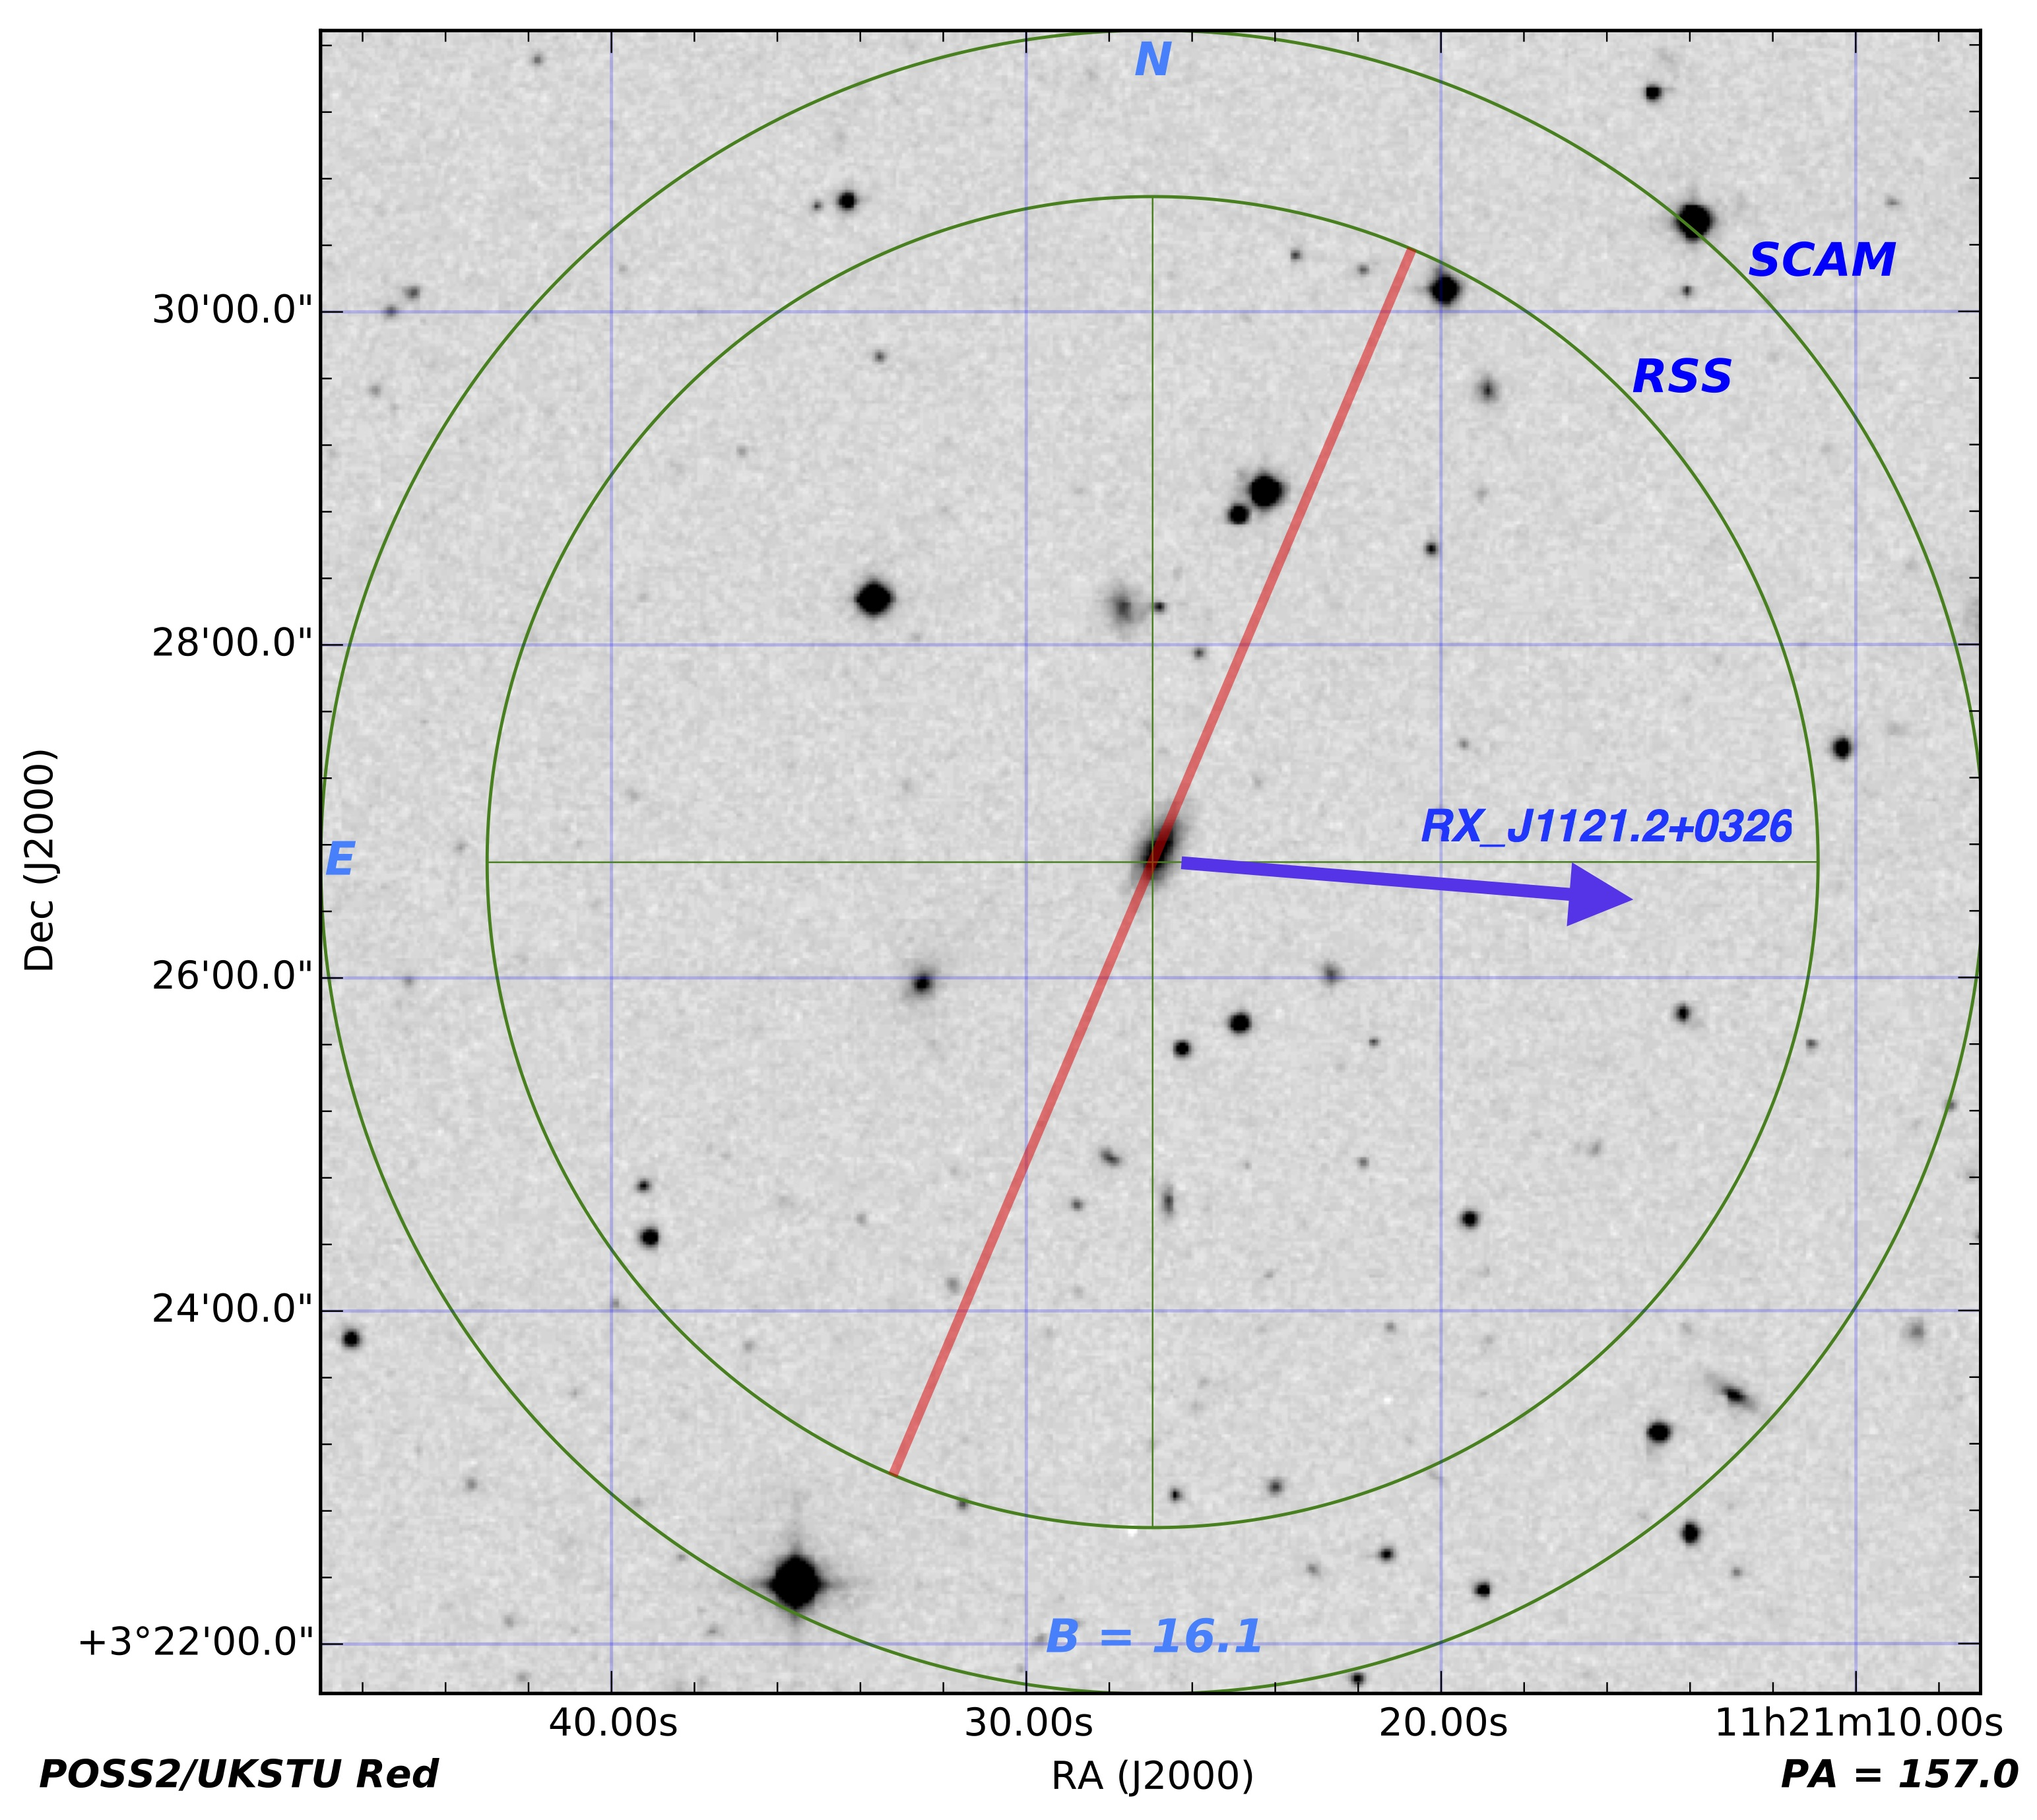
\includegraphics[width=0.45\linewidth]{CGCG039-137_Finding_chart.jpg}\label{finderchart_CGCG039-137}}
  \caption{\small{a) Rotation curve of CGCG039-137. The solid green line indicates the weighted mean velocity over the corresponding x-axis region, and the shaded green indicates the 1$\sigma$ error in the mean. b) SALT finder chart for CGCG039-137 showing the position of the slit in red.}}
\vspace{0pt}
\end{figure}


\subsection{ESO343-G014}
ESO343-G014 is an edge-on ($i = 90^{\circ}$) spiral galaxy with a measured systemic velocity $v_{\rm sys} = 9139 \pm$ 32 \kms. It has a smaller neighboring galaxy, 2MASXJ21372816-3824412, located north of its major axis at a projected distance of 216 kpc and velocity of 9129 \kms. The nearest sightline is towards RBS1768 at $\rho = 466$ kpc and $74^{\circ}$ azimuth angle on the approaching side. We detect 3 blended Ly$\rm \alpha$ absorption components toward RBS1768 at $v_{\rm Ly\alpha} = 9308, 9360, 9434$ \kms~($\Delta v = 169, 221, 295$ \kms). This system is highly blended with galactic S\,{\sc ii}, and therefore their widths are not reliable. All of these are anti-aligned with the rotation of ESO343-G014 relative to the models (cylindrical = [-203, 10], NFW = [-122, 31] \kms). Unfortunately the presence of 2MASXJ21372816-3824412 makes it difficult to attribute this gas uniquely to ESO343-G014. Additionally, this gas could be attributed to either the approaching or receding side of the disk due to the large impact parameter and high azimuth angle of the sightline.

\begin{figure}[ht]
\centering
%  \subfigure[]{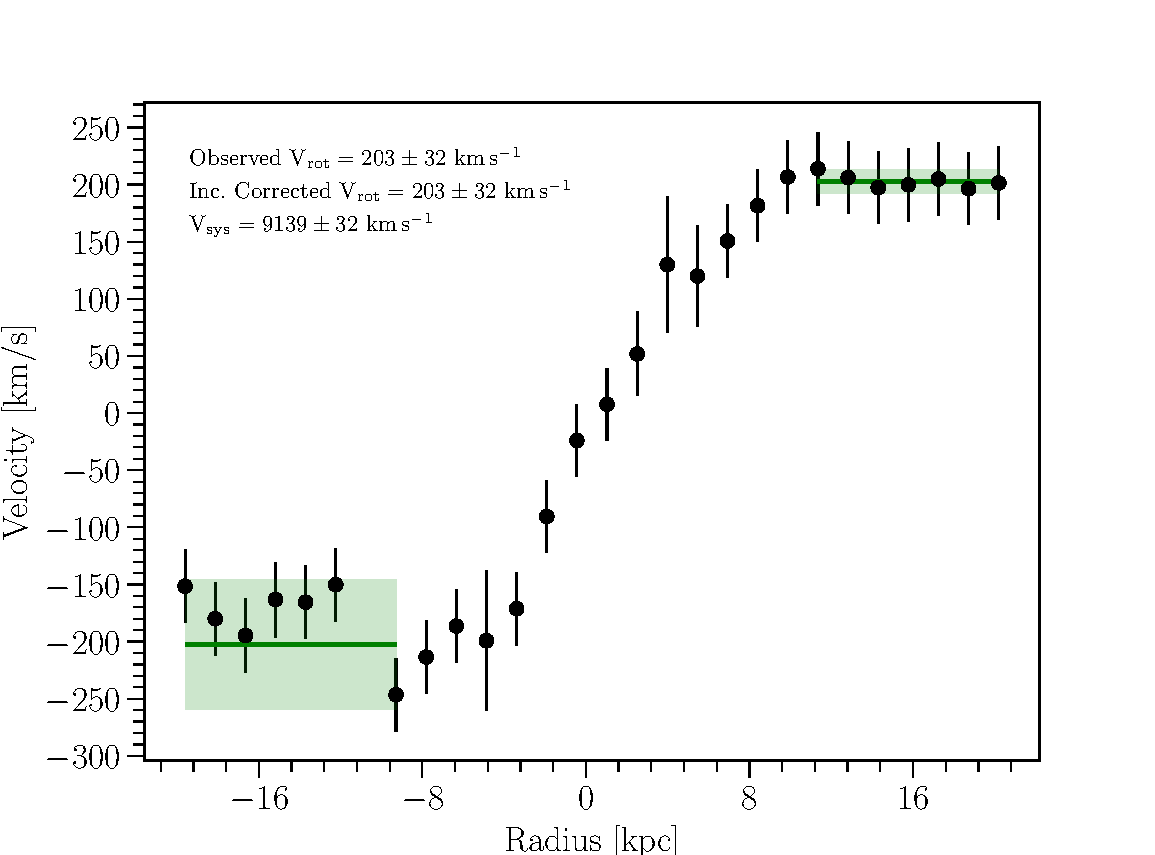
\includegraphics[width=.54\linewidth]{RFGC3781_2_rotation_curve_xphys_helio_vobs_vrotObs_new4.pdf}}{\label{rotationcurve_ESO343-G014}}
  \subfigure[]{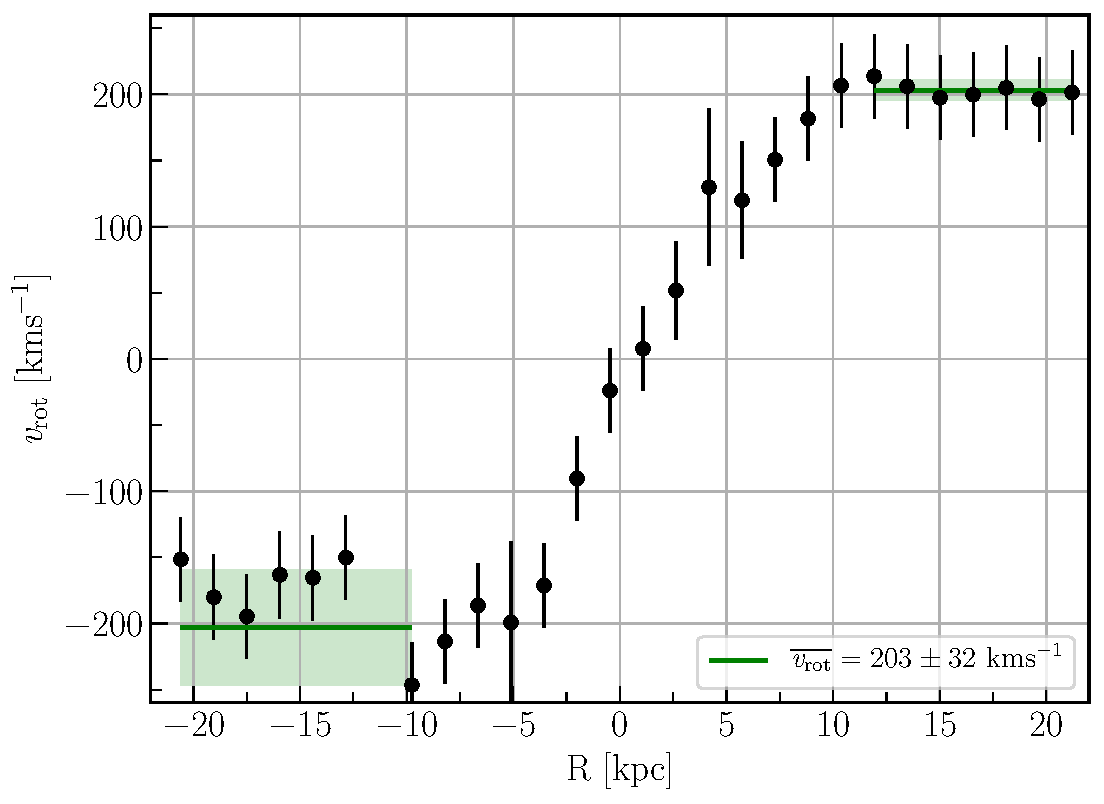
\includegraphics[width=.54\linewidth]{ESO343-G014-rotation_curve_nice3.pdf}}{\label{rotationcurve_ESO343-G014}}
  \subfigure[]{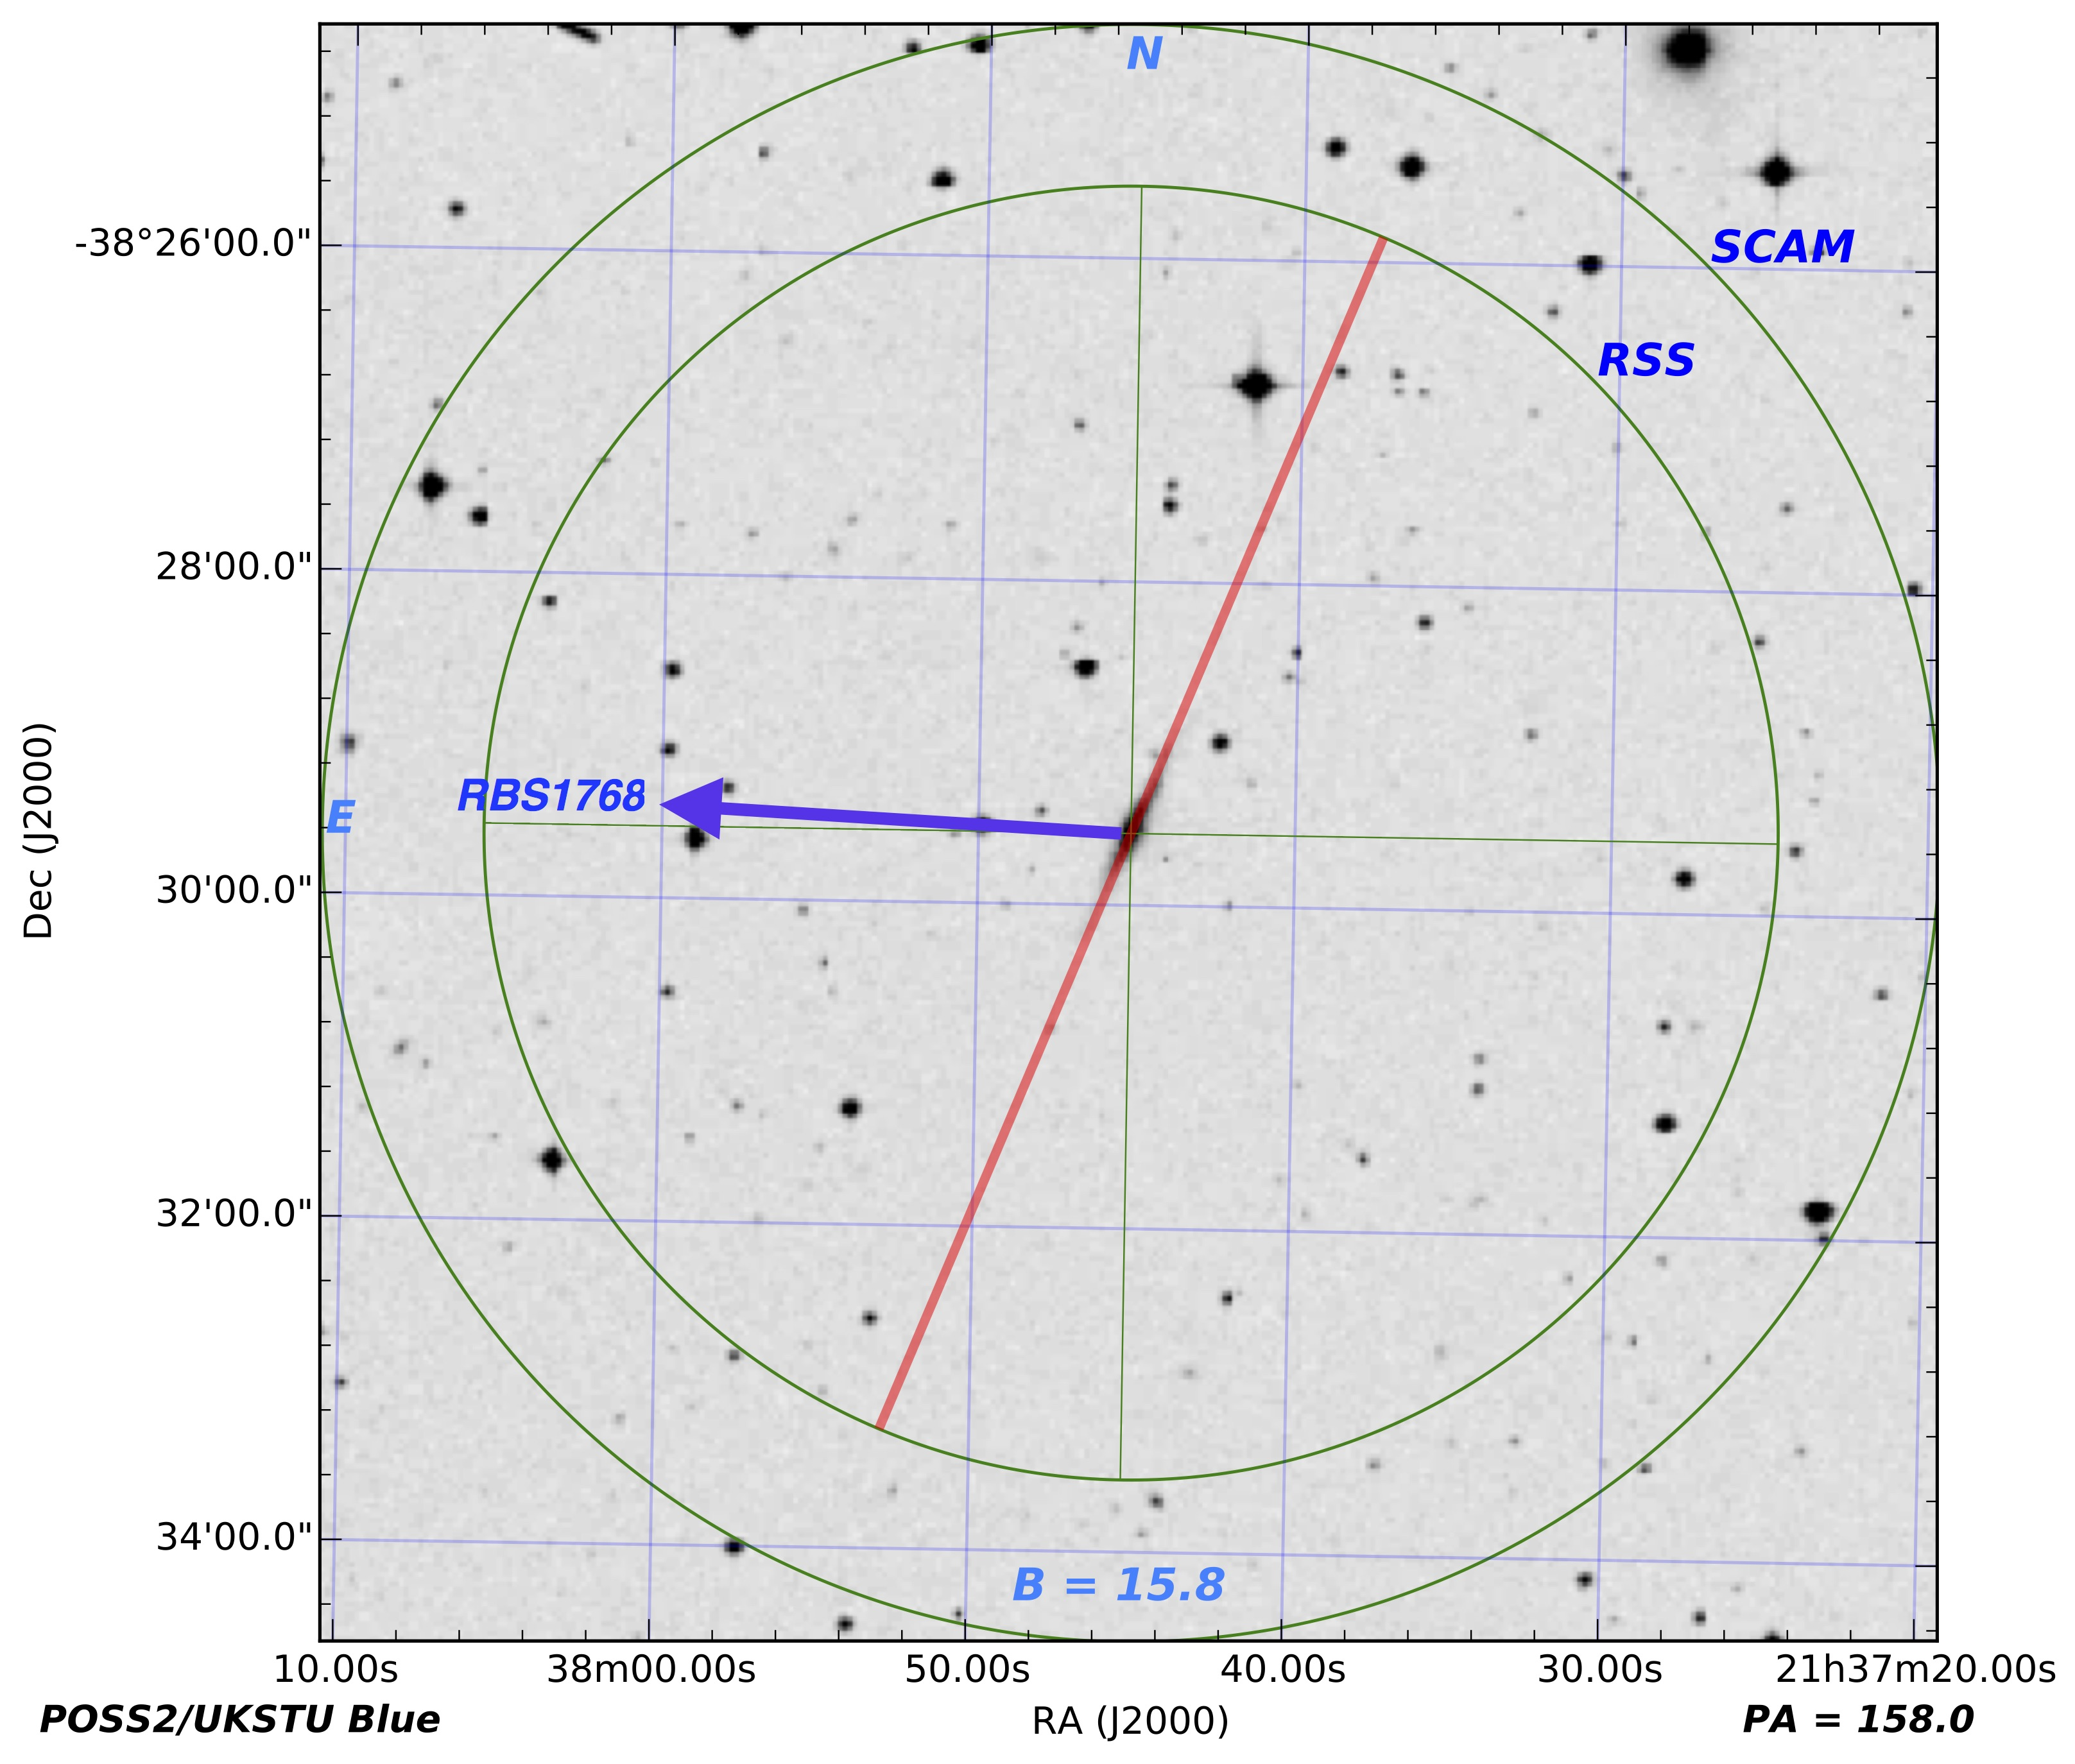
\includegraphics[width=0.45\linewidth]{RFGC3781_FindingChart.jpg}\label{finderchart_ESO343-G014}}
  \caption{\small{a) Rotation curve of ESO343-G014. The solid green line indicates the weighted mean velocity over the corresponding x-axis region, and the shaded green indicates the 1$\sigma$ error in the mean. b) SALT finder chart for ESO343-G014 showing the position of the slit in red.}}
\vspace{0pt}
\end{figure}


\subsection{IC5325}
IC5325 is a mostly face-on ($i = 25^{\circ}$) SAB(rs)bc type galaxy with a measured systemic velocity $v_{\rm sys} = 1512 \pm 8$ \kms. It's inclination is just high enough to obtain a reasonable rotation curve. The closest neighboring galaxy is ESO347-G020 to the southeast at 306 kpc and $v_{sys} = 1745$ \kms. Three other much smaller galaxies are also located $\sim 450$ kpc to the southwest. The background QSO RBS2000 is located northeast at $\rho = 314$ kpc and  $64^{\circ}$ azimuth angle on the approaching side of IC5325. We detect Ly$\alpha$ at $v_{\rm Ly\alpha} = 1598$ \kms~($\Delta v = 86$ \kms) towards RBS2000. While this velocity is anti-aligned with the rotation the disk gas relative to our model predictions (cylindrical = [-41, -20], NFW = [-29, 1] \kms), the low inclination angle of IC5325 leads to a highly uncertain position angle. Without additional observations, we cannot say for certain if the location of RBS2000 actually lies on the approaching or receding side. This position angle uncertainty also means our SALT rotation curve is a lower limit on the true rotation velocity of IC5325.

\begin{figure}[ht]
\centering
%  \subfigure[]{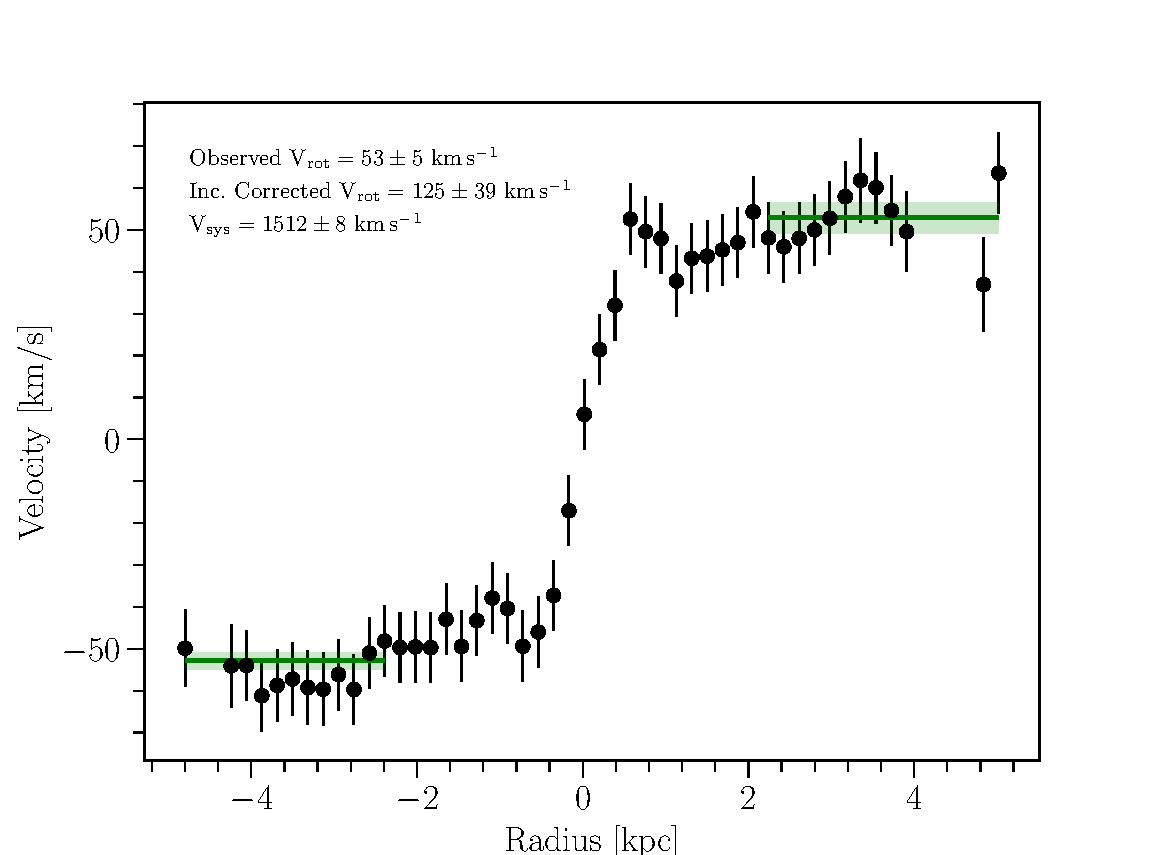
\includegraphics[width=.54\linewidth]{IC5325_2_rotation_curve_xphys_helio_vobs_vrotObs_new4.pdf}}{\label{rotationcurve_IC5325}}
  \subfigure[]{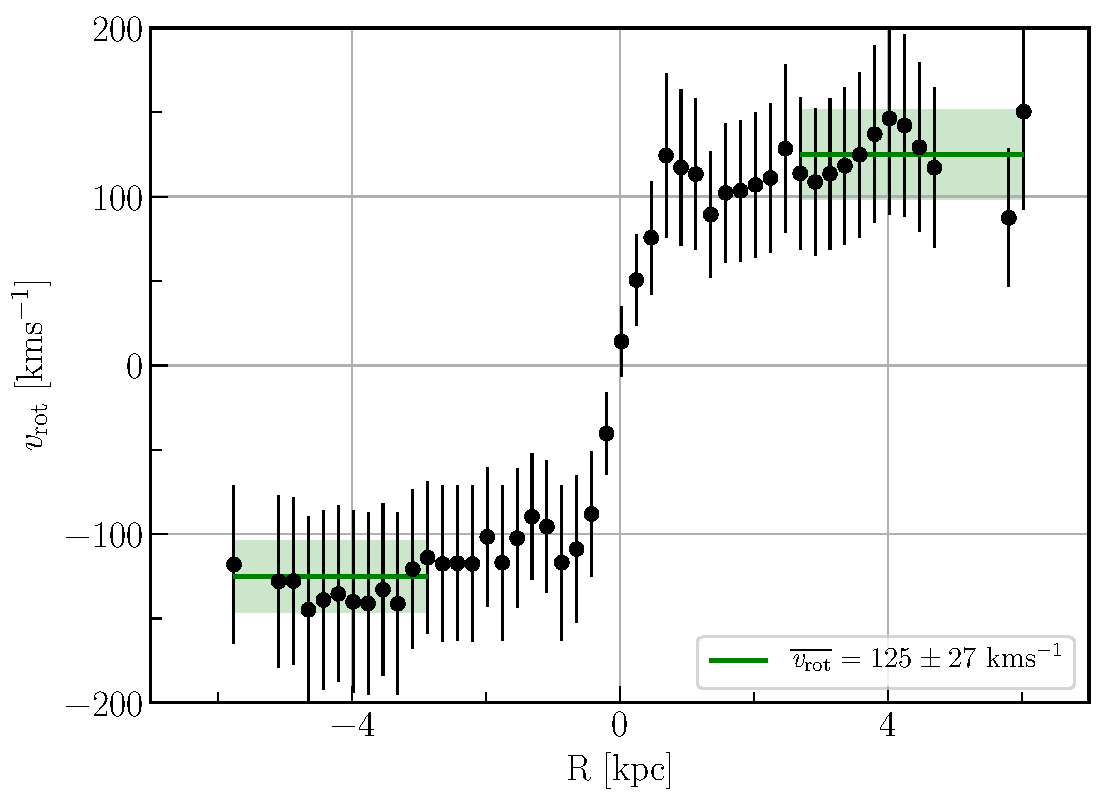
\includegraphics[width=.54\linewidth]{IC5325-rotation_curve_nice3.pdf}}{\label{rotationcurve_IC5325}}
  \subfigure[]{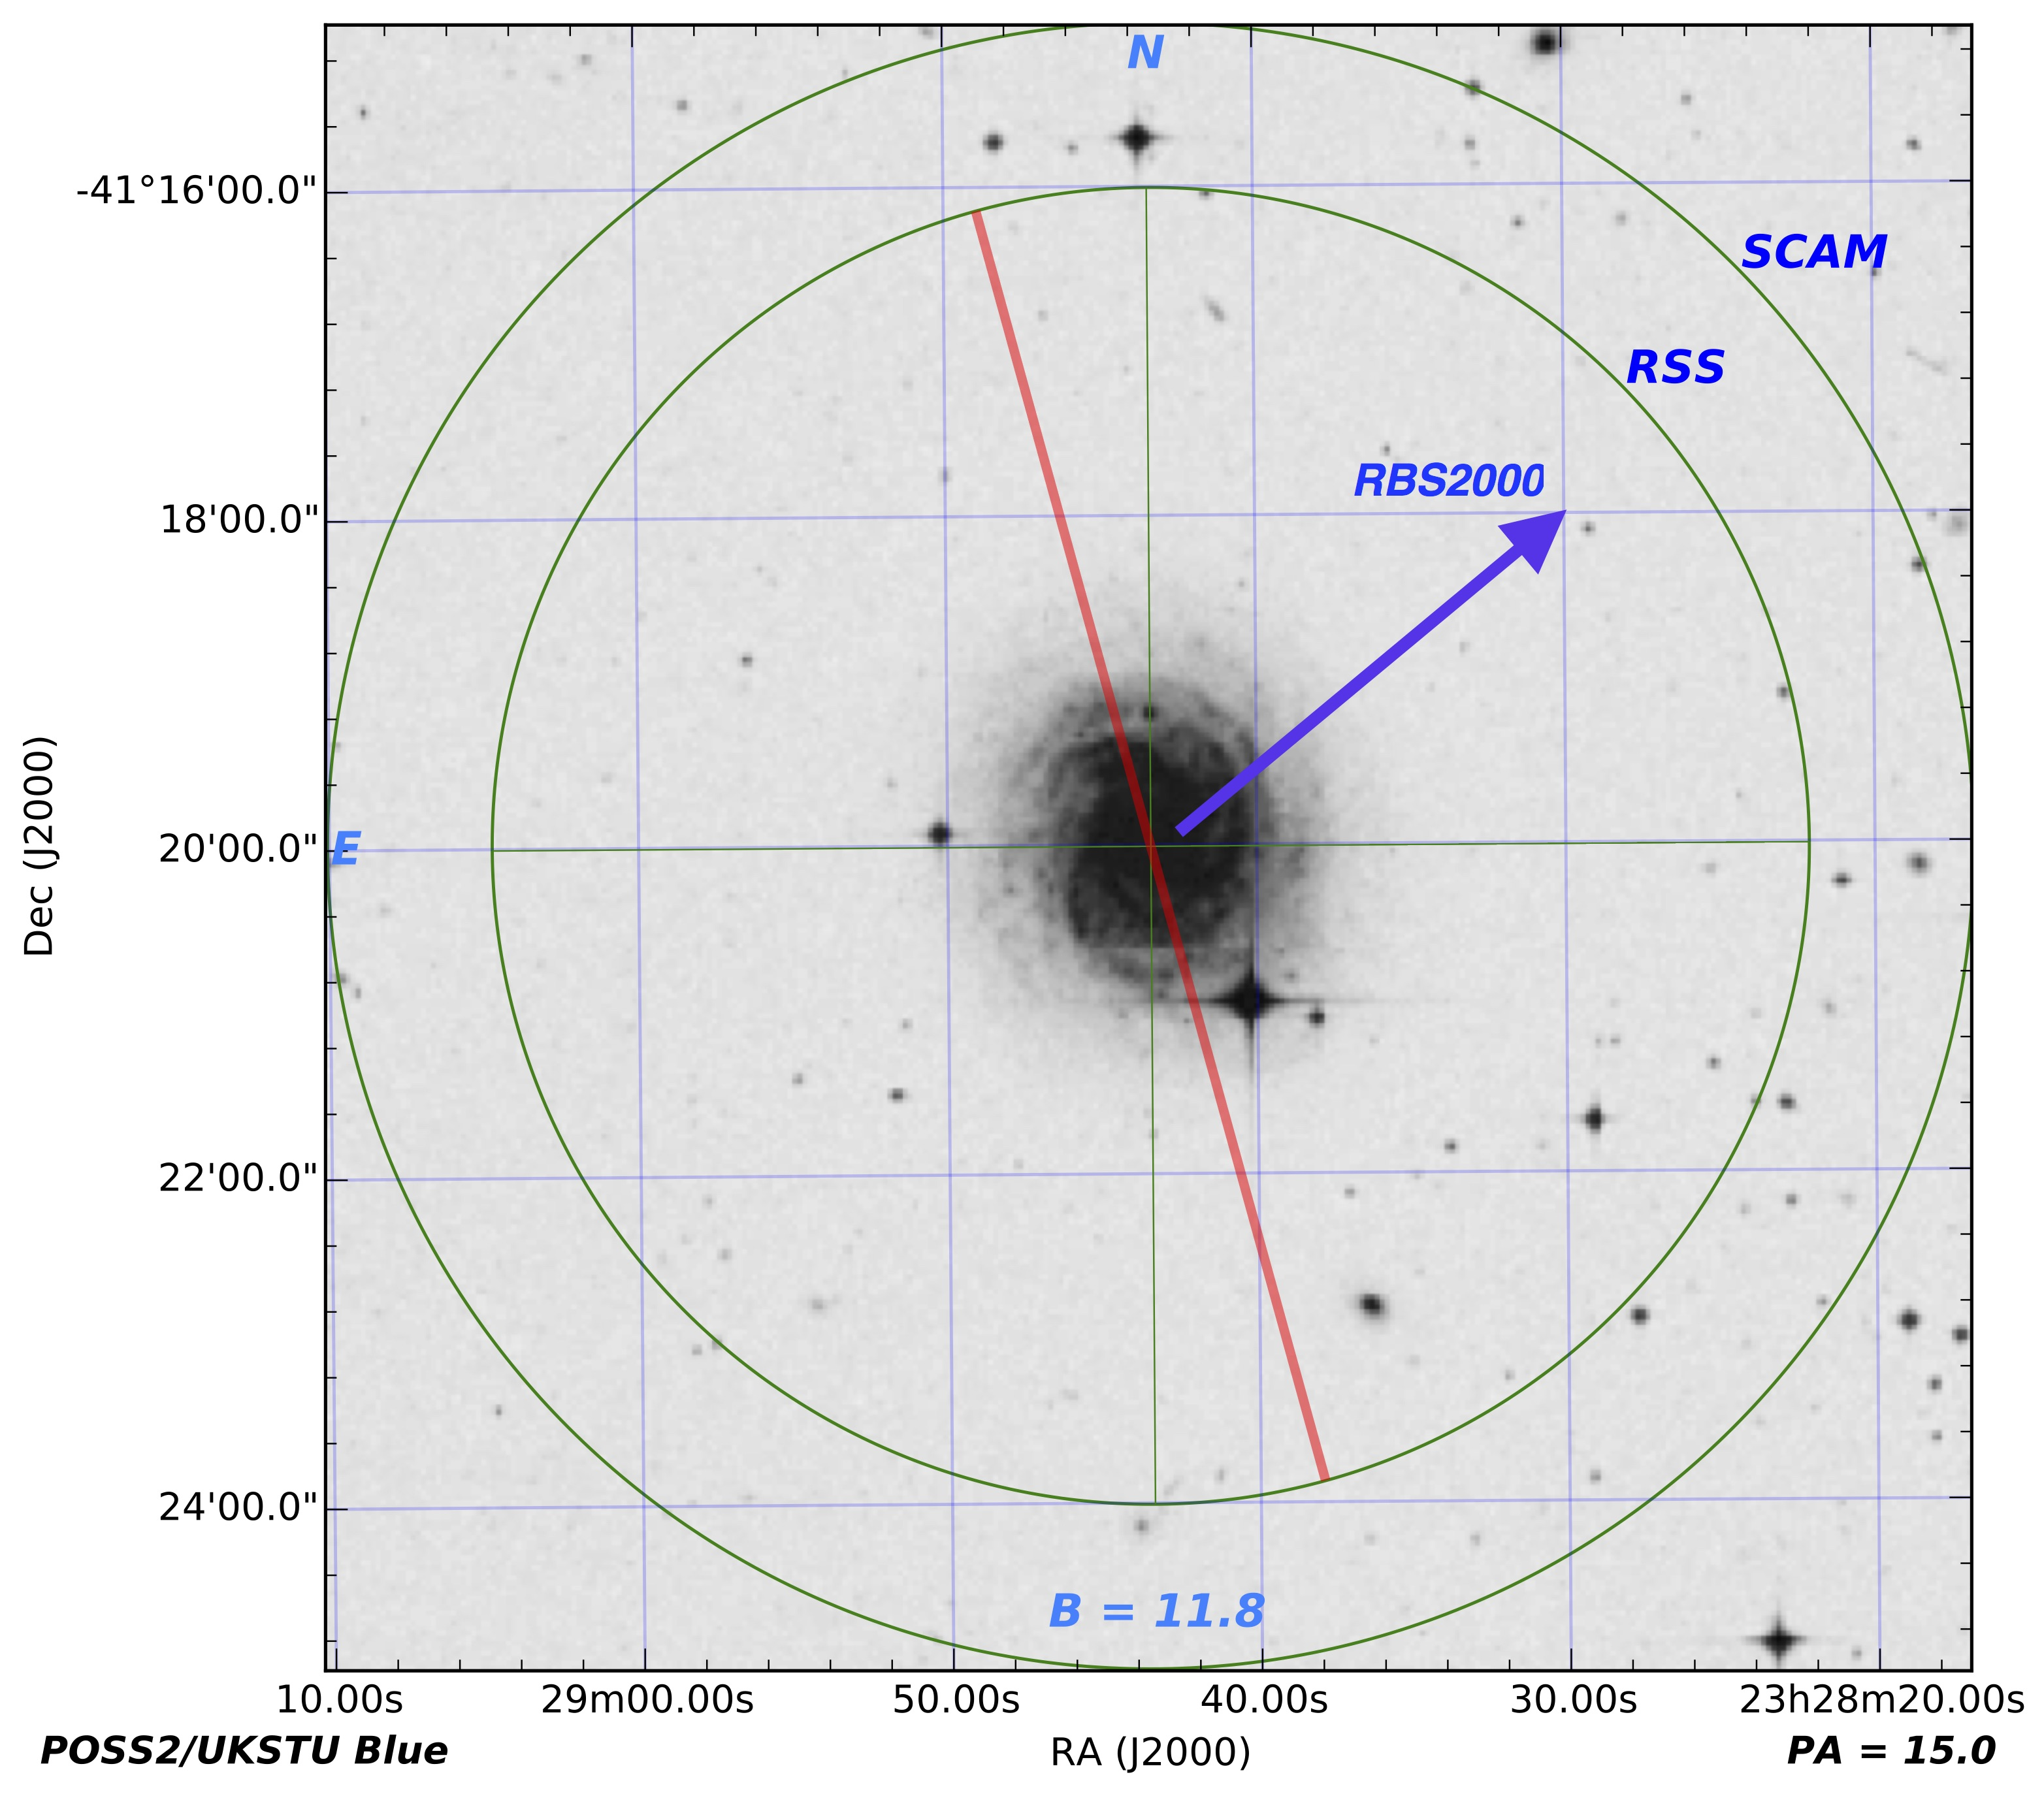
\includegraphics[width=0.45\linewidth]{IC5325_FindingChart.jpg}\label{finderchart_IC5325}}
  \caption{\small{a) Rotation curve of IC5325. The solid green line indicates the weighted mean velocity over the corresponding x-axis region, and the shaded green indicates the 1$\sigma$ error in the mean. b) SALT finder chart for IC5325 showing the position of the slit in red.}}
\vspace{0pt}
\end{figure}



\subsection{MCG-03-58-009}
MCG-03-58-009 is a massive and very isolated Sc type galaxy at a measured systemic velocity of $v_{\rm sys} = 9015 \pm 19$ \kms~and inclination angle of $i = 61^{\circ}$. The background QSO MRC2251-178 is located southeast at $\rho = 355$ kpc at an azimuth angle of $71^{\circ}$ on the receding side. We detect a weak Ly$\rm \alpha$ absorber at $v_{\rm Ly\alpha} = 9029$ \kms~($\Delta v = 14$ \kms) towards MRC2251-178. This absorber velocity falls well within the expected range for co-rotation relative to our models (cylindrical = [-26, 137], NFW = [-42, 83] \kms). Although this absorber matches the velocity expected for co-rotation, the velocity difference ($\Delta v = 14$ \kms) is also within the systemic velocity uncertainty for MCG-03-58-009. The relative weakness of this absorber (EW = $62 \pm 4$ m\AA) is somewhat unusual given it's proximity (just outside of 1 $R_{vir}$) to a massive galaxy. If this is representative of an isolated system such as MCG-03-58-009, then we should expect the halo rotational velocity to approach systemic by 1 $R_{vir}$.

\begin{figure}[ht]
\centering
%  \subfigure[]{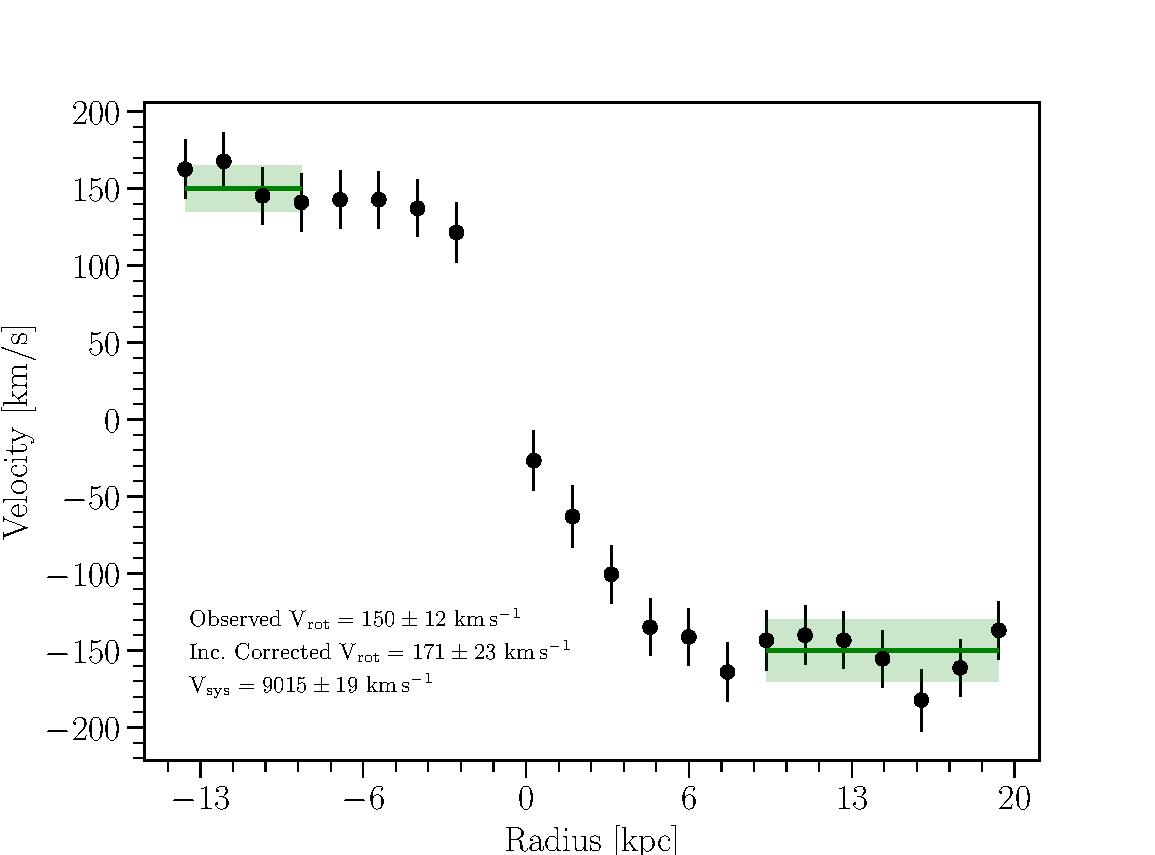
\includegraphics[width=.54\linewidth]{MCG-03-58-009_2_rotation_curve_xphys_helio_vobs_vrotObs_new4.pdf}}{\label{rotationcurve_MCG-03-58-009}}
  \subfigure[]{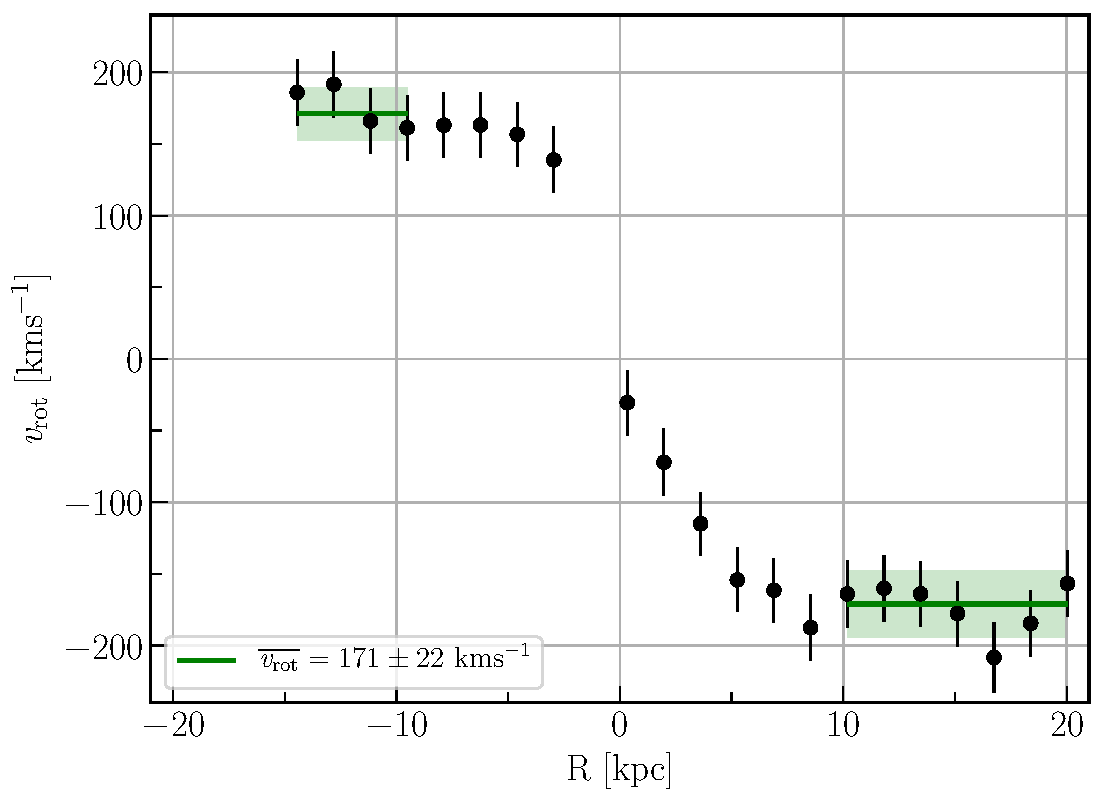
\includegraphics[width=.54\linewidth]{MCG-03-58-009-rotation_curve_nice3.pdf}}{\label{rotationcurve_MCG-03-58-009}}
  \subfigure[]{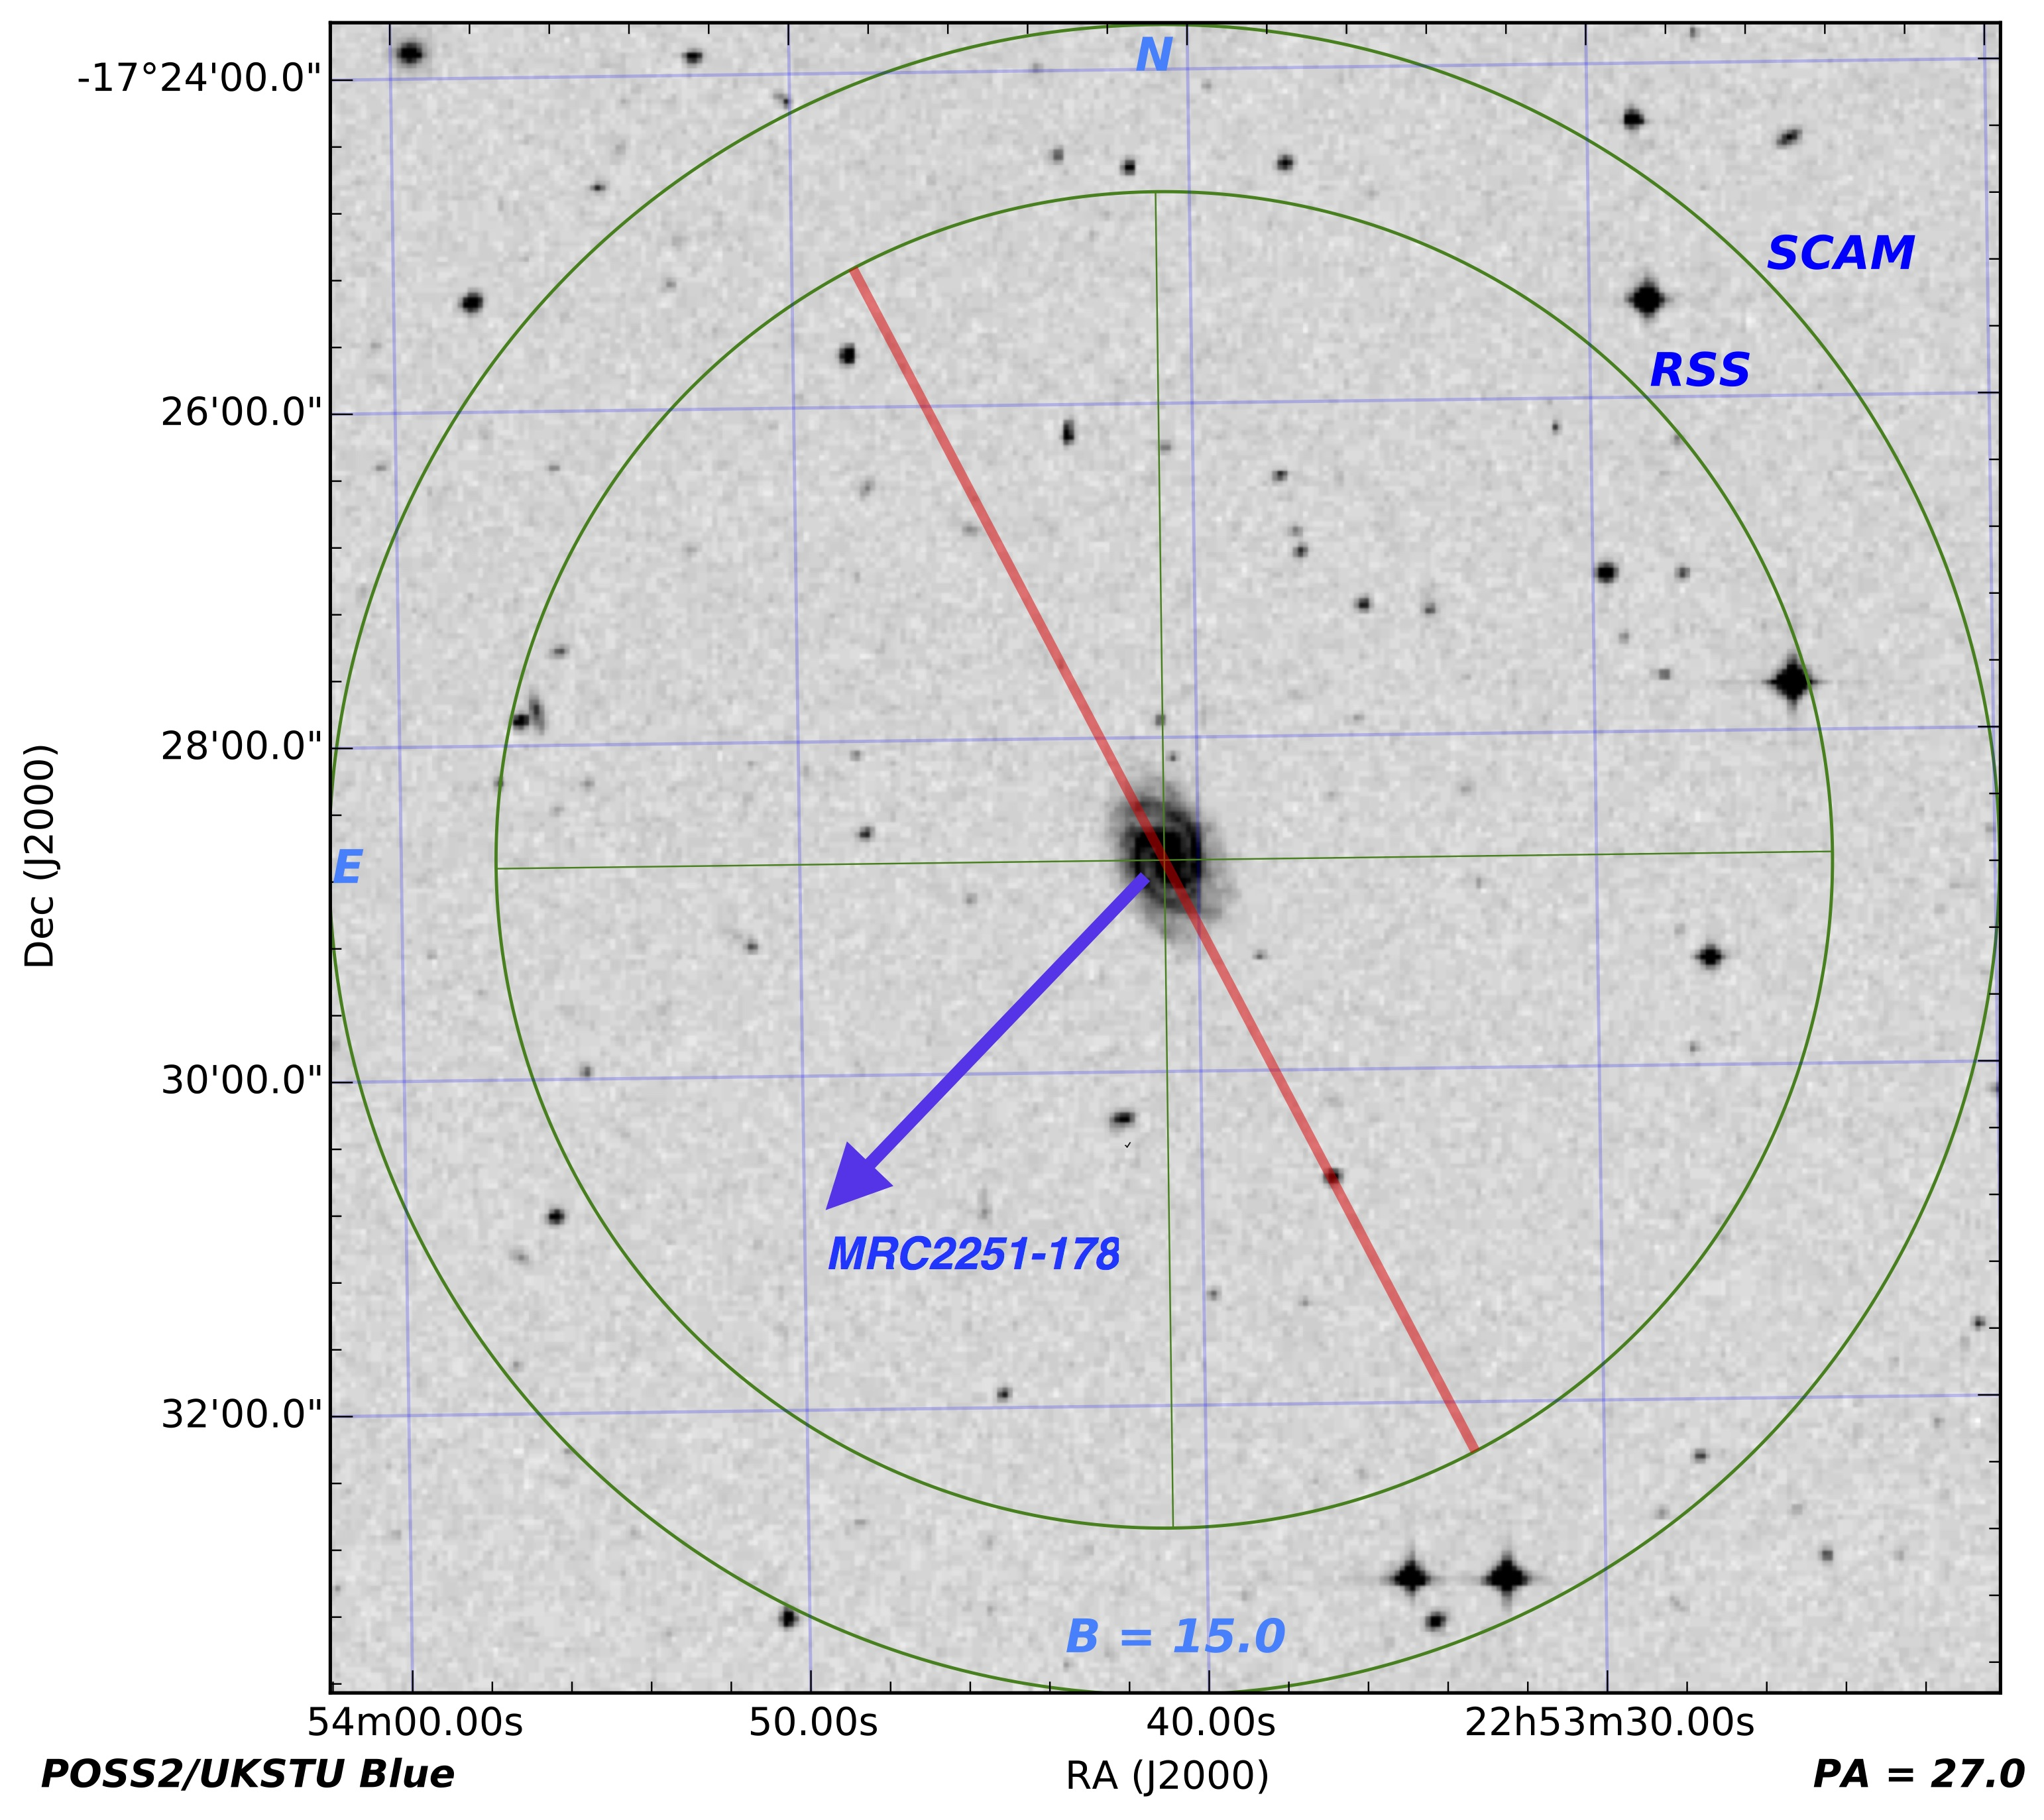
\includegraphics[width=0.45\linewidth]{MCG-03-58-009_FindingChart.jpg}\label{finderchart_MCG-03-58-009}}
  \caption{\small{a) Rotation curve of MCG-03-58-009. The solid green line indicates the weighted mean velocity over the corresponding x-axis region, and the shaded green indicates the 1$\sigma$ error in the mean. b) SALT finder chart for MCG-03-58-009 showing the position of the slit in red.}}
\vspace{0pt}
\end{figure}



\subsection{NGC1566}
NGC1566 is a mostly face-on ($i = 19^{\circ}$) SAB(rs)bc type galaxy with measured systemic velocity of $v_{\rm sys} = 1502 \pm 15$ \kms~and inclination angle of $i = 19^{\circ}$. There are several other large galaxies at $\rho \gtrsim 200$ kpc from NGC1566 (e.g., NGC1549, NGC1596, and NGC1581). The closest QSO sightline is toward HE0429-5343, northeast of NGC1566 at $\rho = 256$ kpc and $60^{\circ}$ azimuth angle. We detect Ly$\rm \alpha$ absorption toward HE0429-5343 at $v_{\rm Ly\alpha} = 1167, 1358$ \kms~($\Delta v = -335, -144$ \kms). Both of these absorbers have the correct velocity \emph{sign}, but we would expect a smaller velocity for co-rotation based on our model results (cylindrical = [-53, -2], NFW = [-22, 17] \kms). Unfortunately NGC1617 is slightly closer to this sightline than NGC1566, at $\rho = 233$ kpc and $v_{\rm sys} = 1063$ \kms, so it is not possible to confidently attribute these absorbers to NGC1566.

A more distant QSO sightline toward 1H0419-577 is located to the south at $\rho = 303$ kpc and just east of the receding side of the major axis at an azimuth angle of $10^{\circ}$. We detect Ly$\rm \alpha$ at $v_{\rm Ly\alpha} = 1123, 1188, 1264$ \kms~($\Delta v = -379, -314, -238$ \kms), all of which are the wrong sign for co-rotation relative to our models (cylindrical = [48, 76], NFW = [-2, 31] \kms). This sightline is \emph{also} actually closer to a small group of galaxies including NGC1549, NGC1546 and NGC1536, all with systemic velocities near $\sim 1200$ \kms. Additionally, this absorber system contains C\,{\sc iii}, C\,{\sc iv}, Si\,{\sc ii}, Si\,{\sc iii}, Si\,{\sc iv} lines. These lines likely are associated with this group rather than with NGC1566. 

\begin{figure}[ht]
\centering
%  \subfigure[]{\includegraphics[width=.54\linewidth]{NGC1566_2_rotation_curve_xphys_helio_vobs_vrotObs_new4.pdf}}{\label{rotationcurve_NGC1566}}
  \subfigure[]{\includegraphics[width=.54\linewidth]{NGC1566-rotation_curve_nice3.pdf}}{\label{rotationcurve_NGC1566}}
  \subfigure[]{\includegraphics[width=0.45\linewidth]{NGC1566_FindingChart.jpg}\label{finderchart_NGC1566}}
  \caption{\small{a) Rotation curve of NGC1566. The solid green line indicates the weighted mean velocity over the corresponding x-axis region, and the shaded green indicates the 1$\sigma$ error in the mean. b) SALT finder chart for NGC1566 showing the position of the slit in red.}}
\vspace{0pt}
\end{figure}


\subsection{NGC3513}
NGC3513 a mostly face-on ($i = 30^{\circ}$) SB(rs)c galaxy with measured systemic velocity $v_{\rm sys} = 1204 \pm 12$ \kms. It has a companion galaxy in NGC3511 at $\rho = 44$ kpc and $v_{\rm sys} = 1109$ \kms~(NGC3513 diameter $D = 22.1$ kpc, NGC3511 diameter $D = 28.1$ kpc). The background QSO H1101-232 is located directly south of the pair at $\rho = 60$ kpc and azimuth angle of $67^{\circ}$ on the receding side. We detect Ly$\rm \alpha$ at $v_{\rm Ly\alpha} = 1182$ \kms~($\Delta v = -22$ \kms) toward H1101-232. NGC3513 appears to be rotating slowly, with a maximal inclination-corrected rotation velocity of $v_{\rm rot} / \sin(\emph{i}) = 22 \pm 24$ \kms. The $\Delta v = -22$ \kms~for this absorber is opposite in sign for co-rotation on the sky and just outside our predicted model velocity range (cylindrical = [-19, 27], NFW = [-19, 28] \kms). Given that NGC3511 is so close, this absorber's velocity is probably subject to a complex velocity field influenced by both NGC3511 and NGC3513. For this reason we have marked this galaxy as ``uncertain" in all map plots and have not included it in our statistical results. This absorber system also contains C\,{\sc iv}, N\,{\sc v}, Si\,{\sc ii}, Si\,{\sc iii}, and Si\,{\sc iv} lines.

\begin{figure}[hb]
\centering
%  \subfigure[]{\includegraphics[width=.54\linewidth]{NGC3513_2_rotation_curve_xphys_helio_vobs_vrotObs_new4.pdf}}{\label{rotationcurve_NGC3513}}
  \subfigure[]{\includegraphics[width=.54\linewidth]{NGC3513-rotation_curve_nice3.pdf}}{\label{rotationcurve_NGC3513}}
  \subfigure[]{\includegraphics[width=0.45\linewidth]{NGC3513_Finding_chart.jpg}\label{finderchart_NGC3513}}
  \caption{\small{a) Rotation curve of NGC3513. The solid green line indicates the weighted mean velocity over the corresponding x-axis region, and the shaded green indicates the 1$\sigma$ error in the mean. b) SALT finder chart for NGC3513 showing the position of the slit in red.}}
\vspace{0pt}
\end{figure}



\subsection{NGC3633}
NGC3633 is an isolated, edge-on ($i = 72^{\circ}$) SAa type galaxy with a measured systemic velocity $v_{\rm sys} = 2587 \pm 7$ \kms. Several locations along the disk of NGC3633 show two velocities for emission. We have combined these into a single velocity measurement via a weighted average. 

The background QSO RX\_J1121.2+0326 is located southeast at $\rho = 184$ kpc and $58^{\circ}$ azimuth on the approaching side of NGC3633. We detect Ly$\rm \alpha$ at $v_{\rm Ly\alpha} = 2605$ \kms~($\Delta v = 18$ \kms) toward RX\_J1121.2+0326. While close to $v_{\rm sys}$, this absorber velocity is just outside our predicted model velocities (cylindrical = [-153, -14], NFW = [-77, 10] \kms). However, this absorber is also very weak and broad, making the velocity center uncertain by at least $\sim 10$ \kms. Taking this along with the uncertainty in $V_{\rm sys}$, this absorber could still be consistent with co-rotation.

\begin{figure}[ht]
\centering
%  \subfigure[]{\includegraphics[width=.54\linewidth]{NGC3633_2_rotation_curve_xphys_helio_vobs_vrotObs_new4.pdf}}{\label{rotationcurve_NGC3633}}
  \subfigure[]{\includegraphics[width=.54\linewidth]{NGC3633-rotation_curve_nice3.pdf}}{\label{rotationcurve_NGC3633}}
  \subfigure[]{\includegraphics[width=0.45\linewidth]{NGC3633_FindingChart.jpg}\label{finderchart_NGC3633}}
  \caption{\small{a) Rotation curve of NGC3633. The solid green line indicates the weighted mean velocity over the corresponding x-axis region, and the shaded green indicates the 1$\sigma$ error in the mean. b) SALT finder chart for NGC3633 showing the position of the slit in red.}}
\vspace{0pt}
\end{figure}


\subsection{NGC4536}
NGC4536 is a SAB(rs)bc type galaxy located in the Virgo Cluster at a measured systemic velocity of $v_{sys} = 1867 \pm 33$ \kms~and inclination $i = 61^{\circ}$. The data on the receding side of NGC4536 is messy, and may include contamination from background sources. Hence, our measured systemic velocity, and thus rotation velocity of $139 \pm 37$ \kms, have relatively high uncertainty. Other published redshift values available from NED and rotation velocities from the HyperLEDA database are broadly consistent with our values, albeit biased slightly lower and higher in velocity, respectively.

There are 2 sightlines to the southwest of NGC4536, both on the receding side of the galaxy. HE1228+0131 at $ \rho = 338$ kpc and $86^{\circ}$ azimuth has 5 Ly$\rm \alpha$ lines: $v_{\rm Ly\alpha} =$ 1495, 1571, 1686, 1721, 1854 \kms~($\Delta v = -$372, -296, -181, -146, -13 \kms). None of these are of the correct orientation for co-rotation relative to our model predictions (cylindrical = [18, 51], NFW = [2, 32] \kms), and all are more likely to be associated with other nearby galaxies, such as NGC4517A, which is slightly closer to these absorbers in impact parameter and velocity than is NGC4536. At $v_{\rm Ly\alpha}  = 1686$ \kms~we also detect C\,{\sc ii}, C\,{\sc iv}, Si\,{\sc ii}, Si\,{\sc iii}, and Si\,{\sc iv}, and at $v_{\rm Ly\alpha}  = 1721$ \kms~we detect Lyman series from Ly$\rm \alpha$ to Ly$\rm \theta$ as well as C\,{\sc ii}, C\,{\sc iii}, C\,{\sc iv}, Si\,{\sc ii}, Si\,{\sc iii}, and Si\,{\sc iv}.

The second nearby sightline is toward 3C273 at $\rho = 344$ kpc and $46^{\circ}$ azimuth angle, and shows 3 Ly$\rm \alpha$ lines at $v_{\rm Ly\alpha} =$ 1580, 2156, 2267 \kms~($\Delta v = -$287, 289, 400 \kms). Two of these are correctly oriented for co-rotation relative to our model predictions (cylindrical = [87, 121], NFW = [5, 41] \kms), but are too high in velocity to make this scenario probable. Overall, given the number of nearby galaxies and their locations, we would expect these absorbers to trace the overall velocity field instead of the halo rotation of any particular galaxy. After this galaxy was included in the SALT observing queue we realized it is actually located in the Virgo cluster, so we have decided to remove it from the statistical sample in this paper but present the observed data here nonetheless.

\begin{figure}[b]
\centering
%  \subfigure[]{\includegraphics[width=.54\linewidth]{NGC4536_2_rotation_curve_xphys_helio_vobs_vrotObs_new4.pdf}}{\label{rotationcurve_NGC4536}}
  \subfigure[]{\includegraphics[width=.54\linewidth]{NGC4536-rotation_curve_nice3.pdf}}{\label{rotationcurve_NGC4536}}
  \subfigure[]{\includegraphics[width=0.45\linewidth]{NGC4536_FindingChart.jpg}\label{finderchart_NGC4536}}
  \caption{\small{a) Rotation curve of NGC4536. The solid green line indicates the weighted mean velocity over the corresponding x-axis region, and the shaded green indicates the 1$\sigma$ error in the mean. b) SALT finder chart for NGC4536 showing the position of the slit in red.}}
\vspace{0pt}
\end{figure}

% I removed this weird data on the left side in NGC4536-summary.json, which I then used for the model and NFW fit. 


\subsection{NGC4939}
NGC4939 is a large SA(s)bc type galaxy with measured systemic velocity $v_{\rm sys} = 3093 \pm 33$ \kms~and inclination $i = 61^{\circ}$. The background QSO PG1302-102 is located southeast at $\rho = 254$ kpc and $61^{\circ}$ azimuth angle on the approaching side of NGC4939. We detect a Ly$\rm \alpha$ absorber at $v_{\rm Ly\alpha} = 3448$ \kms~($\Delta v = 355$\kms) towards PG1302-102. As this absorber is located on the approaching side, we can easily rule out co-rotation in this case. NGC4939 does not have any close neighbors, so represents an intriguing case against co-rotation for gas past $1 R_{\rm vir}$.

\begin{figure}[ht!]
\centering
%  \subfigure[]{\includegraphics[width=.54\linewidth]{NGC4939_2_rotation_curve_xphys_helio_vobs_vrotObs_new4.pdf}}{\label{rotationcurve_NGC4939}}
  \subfigure[]{\includegraphics[width=.54\linewidth]{NGC4939-rotation_curve_nice3.pdf}}{\label{rotationcurve_NGC4939}}
  \subfigure[]{\includegraphics[width=0.45\linewidth]{NGC4939_FindingChart.jpg}\label{finderchart_NGC4939}}
  \caption{\small{a) Rotation curve of NGC4939. The solid green line indicates the weighted mean velocity over the corresponding x-axis region, and the shaded green indicates the 1$\sigma$ error in the mean. b) SALT finder chart for NGC4939 showing the position of the slit in red.}}
\vspace{0pt}
\end{figure}

% Originally used an inclination of 48, seems too low.


\subsection{NGC5364}
NGC5364 is a SA(rs)bc pec type galaxy at a measured systemic velocity $v_{\rm sys} = 1238 \pm 17$ \kms~and inclination $i = 57^{\circ}$. It is located in a group environment with 5 other large, nearby galaxies. The background QSO SDSSJ135726.27+043541.4 is located southeast at $\rho = 165$ kpc and $84^{\circ}$ azimuth angle on the receding side of NGC5364. We detect Ly$\rm \alpha$ at $v_{\rm Ly\alpha} = 967, 1124$ \kms~($\Delta v = -271, -114$ \kms) toward SDSSJ135726.27+043541.4. These absorbers have the opposite sign for co-rotation relative to our model predictions (cylindrical = [-26, 108], NFW = [-30, 68] \kms). However, because of the orientation of NGC5364 on the sky with respect to this sightline, these absorbers lie extremely close to the inflection point where projected rotation velocities flip to approaching instead of receding. For example, shifting the location of SDSSJ135726.27+043541.4 east by a tenth of a degree ($\sim 20$ kpc) is sufficient to put these absorbers on the approaching side of NGC5364. Hence, both of these absorbers could be co-rotating with NGC5364 given very reasonable assumptions on the shape of an extended disk. Nonetheless, the fact that this system lives in galaxy group environment likely dominates the surrounding velocity field.
\begin{figure}[ht!]
\centering
%  \subfigure[]{\includegraphics[width=.54\linewidth]{NGC5364_2_rotation_curve_xphys_helio_vobs_vrotObs_new4.pdf}}{\label{rotationcurve_NGC5364}}
  \subfigure[]{\includegraphics[width=.54\linewidth]{NGC5364-rotation_curve_nice3.pdf}}{\label{rotationcurve_NGC5364}}
  \subfigure[]{\includegraphics[width=0.45\linewidth]{NGC5364_FindingChart.jpg}\label{finderchart_NGC5364}}
  \caption{\small{a) Rotation curve of NGC5364. The solid green line indicates the weighted mean velocity over the corresponding x-axis region, and the shaded green indicates the 1$\sigma$ error in the mean. b) SALT finder chart for NGC5364 showing the position of the slit in red.}}
\vspace{0pt}
\end{figure}


\subsection{NGC5786}
NGC5786 is a large, strongly-barred spiral galaxy with measured systemic velocity $v_{\rm sys} = 2975 \pm 22$ \kms~and inclination $i = 65^{\circ}$. The background QSO QSO1500-4140 is located directly east at $\rho = 453$ kpc and $1^{\circ}$ azimuth angle on the receding side of NGC5786. We detect Ly$\rm \alpha$ at $v_{\rm Ly\alpha} = 3138$ \kms~($\Delta v = 163$ \kms) toward QSO1500-4140, which is slightly above the model predicted velocity range (cylindrical = [106, 160], NFW = [19, 67] \kms). However, the two neighboring galaxies ESO327-G038 and ESO327-G039 are both located south of NGC5786 at $\rho = 62, 296$ kpc, respectively. These nearby galaxies, along with the large distance to the absorption ($\sim 2.5 R_{\rm vir}$), make it difficult to believe there is a connection to a NGC5786 extended disk.

\begin{figure}[ht]
\centering
%  \subfigure[]{\includegraphics[width=.54\linewidth]{NGC5786_2_rotation_curve_xphys_helio_vobs_vrotObs_new4.pdf}}{\label{rotationcurve_NGC5786}}
  \subfigure[]{\includegraphics[width=.54\linewidth]{NGC5786-rotation_curve_nice3.pdf}}{\label{rotationcurve_NGC5786}}
  \subfigure[]{\includegraphics[width=0.45\linewidth]{NGC5786_FindingChart.jpg}\label{finderchart_NGC5786}}
  \caption{\small{a) Rotation curve of NGC5786. The solid green line indicates the weighted mean velocity over the corresponding x-axis region, and the shaded green indicates the 1$\sigma$ error in the mean. b) SALT finder chart for NGC5786 showing the position of the slit in red.}}
\vspace{0pt}
\end{figure}


\subsection{UGC09760}
UGC09760 is an edge-on ($i = 90^{\circ}$), slow-rotating Sd galaxy with measured systemic velocity $v_{\rm sys} =  2094 \pm 16$ \kms. This systemic velocity deviates slightly from other published redshifts, such as the The Updated Zwicky Catalog value of $v_{\rm sys} = 2023 \pm 2$ \kms~\citep{falco1999}. This is likely due to our method of imposing rotation symmetry and averaging the approaching and receding velocities to derive $v_{\rm sys}$. If we do not sample the rotation curve far enough out, a systematic offset is not unreasonable. Indeed, we do not detect the rotation curve turnover or flattening point.

The background QSO SDSSJ151237.15+012846.0 is located southeast at $\rho = 123$ kpc and $90^{\circ}$ azimuth angle. We detect Ly$\rm \alpha$ absorption at $v_{\rm Ly\alpha} = 2029$ \kms~($\Delta v = -65$ \kms) toward SDSSJ151237.15+012846.0. This velocity falls outside the model predictions for co-rotation (cylindrical = [-30, 30], NFW = [-30, 86] \kms), but unfortunately this sightline lies almost exactly at an azimuth of $90^{\circ}$. Hence, the motion of this gas could easily be either co-rotating or counter-rotating depending on a minute change in the position angle assigned to UGC09760. This is especially true if we assume our measured $v_{sys}$ is erroneously high, and indeed closer to the values obtained by other observations. For example, if we adjust the position angle by a single degree, to $56^{\circ}$ instead of $57^{\circ}$, our model predictions become (cylindrical = [-30, 30] , NFW = [-79, 30] \kms) and this absorber becomes consistent with co-rotation in the NFW model.

It is worth noting that there are several small satellite galaxies nearby, including SDSSJ151208.16+013508.5, SDSSJ151121.63+013637.6, SDSSJ151241.38+013723.7 and UGC09746 (impact parameters $\rho = 53, 88, 82, 230$ kpc respectively). All of these galaxies lie slightly blue-ward of UGC09760, and thus \emph{farther} away in velocity from the Ly$\rm \alpha$ absorber at 2029 \kms.

\begin{figure}[ht]
\centering
%  \subfigure[]{\includegraphics[width=.54\linewidth]{UGC09760_2_rotation_curve_xphys_helio_vobs_vrotObs_new4.pdf}}{\label{rotationcurve_UGC09760}}
  \subfigure[]{\includegraphics[width=.54\linewidth]{UGC09760-rotation_curve_nice3.pdf}}{\label{rotationcurve_UGC09760}}
  \subfigure[]{\includegraphics[width=0.45\linewidth]{UGC09760_FindingChart.jpg}\label{finderchart_UGC09760}}
  \caption{\small{a) Rotation curve of UGC09760. The solid green line indicates the weighted mean velocity over the corresponding x-axis region, and the shaded green indicates the 1$\sigma$ error in the mean. b) SALT finder chart for UGC09760 showing the position of the slit in red.}}
\vspace{0pt}
\end{figure}



\section{Ancillary Data} \label{ancillary_data}
To increase our sample size we have also searched the literature for galaxies with published rotation curves and orientations. Unfortunately, while the rotation velocity is available for thousands of galaxies, only a handful of publications also include the \emph{orientation} of the rotation on the sky. Of these, we were able to find 18 additional galaxies which have a systemic velocity greater than $\sim 500$ \kms, and are near to a COS or STIS sightline with available data. We have included 3 of the galaxy-QSO systems analyzed by \cite{cote2005}. We briefly summarize each of these systems here (see Sections \ref{NGC6140} - \ref{UGC04238}), and refer the reader to \cite{cote2005} for a more complete discussion. As new spectra and redshift-independent distances are available for these systems our results, while similar, are not identical.


\subsection{NGC2770}
NGC2770 is a large, edge-on ($i = 80^{\circ}$) Sc type galaxy with systemic velocity $v_{\rm sys} = 1948 \pm 2$ \kms. It is mostly isolated except for two nearby small dwarfs MCG+06-20-036NED02 and GALEXASCJ090946.88+330840.4 (both 25 kpc away, on opposite sides of NGC2770). We take the rotation curve and orientation information produced by \cite{rhee1996}.  There are five nearby QSOs, which we present in order of increasing impact parameter. 

First, the QSO FBQSJ0908+3246 is located south at $\rho = 204$ kpc and $59^{\circ}$ azimuth angle on the approaching side of NGC2770. We detect Ly$\rm \alpha$ at $v_{\rm Ly\alpha} = 1915, 1982$ \kms~($\Delta v = -33, 34$ \kms). Relative to our model predictions (cylindrical = [-146, -4], NFW = [-117, 10] \kms), only the lower velocity line can be described as co-rotating.

Second, the QSO TON1015 is located northeast at $\rho = 218$ kpc and $61^{\circ}$ azimuth angle on the receding side of NGC2770. We detect Ly$\rm \alpha$ at $v_{\rm Ly\alpha} = 1833, 1985$ \kms~($\Delta v = -115, 37$ \kms). Relative to our model predictions (cylindrical = [3, 146], NFW = [-10, 115] \kms), only the higher velocity absorber can be described as co-rotating.

Third the QSO SDSSJ091127.30+325337.0 is located southeast at $\rho = 234$ kpc and $30^{\circ}$ azimuth angle on the approaching side of NGC2770. We detect Ly$\rm \alpha$ at $v_{\rm Ly\alpha} = 2063$ \kms~($\Delta v = 115$ \kms). Relative to our model predictions (cylindrical = [-150, -43], NFW = [-117, -19] \kms), this absorber appears to be counter-rotating.

Fourth, the QSO SDSSJ091052.80+333008.0 at is located northeast at $\rho = 239$ kpc and $66^{\circ}$ azimuth angle on the receding side of NGC2770. We detect Ly$\rm \alpha$ at $v_{\rm sys} = 1824, 1975$ \kms~($\Delta v = -124, 27$ \kms). Relative to our model predictions (cylindrical = [6, 145], NFW = [-7, 112] \kms), only the higher velocity absorber can be described as co-rotating.

Finally, the QSO TON1009 is located south at $\rho = 267$ kpc and $41^{\circ}$ azimuth angle on the approaching side of NGC2770. We detect Ly$\rm \alpha$ at $v_{\rm sys} = 1908, 1980$ \kms~($\Delta v = -40, 32$ \kms). Relative to our model predictions (cylindrical = [-146, -39], NFW = [-110, -14] \kms), only the lower velocity absorber can be described as co-rotating.

Interestingly, we appear to be detecting extended gas structures in these 5 sightlines. Toward the northeast we find TON1015 and SDSSJ091052.80+333008.0 and a set of absorber pairs at $v_{\rm Ly\alpha} =1833, 1824$ \kms~and $v_{\rm Ly\alpha} = 1985, 1975$ \kms~each having very similar EW and $N_{\rm \HI}$, and remarkably similar appearing line-structure. Adopting a distance of 28.6 Mpc to this cloud, we calculate a linear separation between TON1015 and SDSSJ091052.80+333008.0 of 28 kpc. Hence, there appears to be two distinct clouds of at least 28 kpc in physical extent sandwiched around the systemic velocity of NGC2770. Toward the south we find TON1009 and FBQSJ0908+3246 and a set of absorber pairs at $v_{\rm Ly\alpha} =1908, 1915$ \kms~and $v_{\rm Ly\alpha} = 1980, 1982$ \kms, again with similar EW, $N_{\rm \HI}$ and line-shapes.



\subsection{NGC3067}
NGC3067 is a mostly edge-on ($i = 71^{\circ}$) SAB(s)ab type galaxy with systemic velocity $v_{\rm sys} = 1465 \pm 5$ \kms. This galaxy and the nearby QSO sightline toward 3C232 is a particularly well studied system. They are separated by only $\rho = 11$ kpc ($74^{\circ}$ azimuth angle on the northwest, receding side) and a Lyman Limit System (LLS) with column density $N_{\scriptsize \HI} = 1 \times 10^{20}$ $\rm cm^{-2}$ is detected toward 3C232 at $v_{\rm Ly\alpha} = 1408$ \kms, which has been postulated as a high velocity cloud (HVC) orbiting NGC3067 \citep{carilli1989, keeney2005}. 

We obtained the rotation curve for NGC3067 from \cite{rubin1982} and the orientation from \cite{carilli1989}. While \HI~measurements of this LLS fit a single component (at $v_{\rm H\I} =1421$ \kms), we have fit 3 separate components at $v_{\rm Ly\alpha} = 1408, 1510, 1641$ \kms~($\Delta v = -57, 45, 176$ \kms) to match the associated metal lines (namely, C\,{\sc iv}, Si\,{\sc ii}, Si\,{\sc iii}, Si\,{\sc iv}, Mg\,{\sc ii}, Fe\,{\sc ii}, and N\,{\sc i} all show at least 2 separate components). This splitting has been analyzed in detail most recently by \cite{keeney2005} and \cite{stocke2010}, who find similar but slightly lower $v_{\rm Ly\alpha}$ for all three absorbers. Only the lowest velocity component can strictly be described by our model velocity range (cylindrical = [-121, 25], NFW = [-139, 26] \kms), however the $v_{\rm Ly\alpha} = 1510$ \kms~component is also very close to this range. The $v_{\rm Ly\alpha} = 1641$ \kms~component, however, must be either a counter-rotating cloudlet or an outflow directed away from our line of sight.

A second QSO SDSSJ095914.80+320357.0 is located farther away, to the southeast at $\rho = 128$ kpc and $43^{\circ}$ azimuth angle on the receding side of NGC3067. We detect Ly$\rm \alpha$ at v$_{\rm Ly\alpha} = 1493$ \kms~($\Delta v = 28$ \kms), which agrees well with our model predicted velocity range (cylindrical = [11, 138], NFW = [-12, 81] \kms).



\subsection{NGC3198}
NGC3198 is a SB(rs)c type galaxy with systemic velocity $v_{\rm sys} = 660 \pm 1$ \kms and inclination = $i = 73^{\circ}$. It is a well studied galaxy, and is included in the detailed THINGS rotation curve study of \cite{deblok2008}. We extracted the raw rotation curve derived by \cite{deblok2008} using the plot digitization software WebPlotDigitizer\footnote{WebPlotDigitizer; http://arohatgi.info/WebPlotDigitizer}. NGC3198 has an even and flat rotation curve, with an average velocity of $v_{\rm rot} = 152$ \kms. The background QSO RX\_1017.5+4702 is located northeast at $\rho = 370$ kpc and $55^{\circ}$ azimuth angle on the approaching side of NGC3198. We detect Ly$\rm \alpha$ toward RX\_1017.5+4702 at $v_{\rm Ly\alpha} = 629$ \kms~($\Delta v = -32$ \kms), which can nicely be described by a co-rotating disk based on our model predicted velocity range (cylindrical = [-153, -21], NFW = [-91, 6] \kms). We note that the small dwarf galaxy SDSSJ101848.77+452137.0 is located 65 kpc away from NGC3198 toward the southwest.



\subsection{NGC3351}
NGC3351 is a mostly face-on ($i = 42^{\circ}$) SB(r)b type galaxy with systemic velocity  $v_{\rm sys} = 778 \pm 4$ \kms. It is located $\sim200$ kpc southwest of the core of the Leo I group. We take the rotation curve and orientation produced by \cite{dicaire2008}. While we expect any extended disk rotation to be quickly disrupted due to the complex Leo I environment, this galaxy also has one of the closest sightlines in our sample with SDSSJ104335.90+115129.0 at $\rho = 31$ kpc and $13^{\circ}$ azimuth on the northwest, approaching side. We detect Ly$\rm \alpha$ at $v_{\rm Ly\alpha} = 717, 882, 1030$ \kms ($\Delta v = -61, 104, 252$ \kms) toward this sightline. The lowest velocity absorber agrees nicely with both models for co-rotation, while the other two are above our model predictions (cylindrical = [-99, 12], NFW = [-68, 20] \kms). We also detect multiple metal ions associated with the $v_{\rm Ly\alpha} = 717$ \kms~line, including C\,{\sc ii}, N\,{\sc i}, N\,{\sc v}, O\,{\sc i}, Si\,{\sc ii}, Si\,{\sc iii}, Si\,{\sc iv}, S\,{\sc ii}, and Fe\,{\sc ii}.



\subsection{NGC3432}
NGC3432 is an edge-on ($i = 90^{\circ}$) SB(s)m type galaxy with systemic velocity $v_{\rm sys} = 616 \pm 4$ \kms. It is interacting with the nearby dwarf galaxy UGC05983 located 11 kpc away and at $v_{\rm sys} = 765$ \kms. We take a rotation curve and orientation for NGC3432 from \cite{rhee1996}. The QSO CSO295 is located just 20 kpc away and just to the receding side of the minor axis ($82^{\circ}$ azimuth angle). This is the second closest pair in our sample, after the 11 kpc separated NGC3067-3C232 system. We detect Ly$\rm \alpha$ at $v_{\rm Ly\alpha} = 600, 662$ \kms~($\Delta v = -16, 46$ \kms) toward CSO295. Relative to our model predictions (cylindrical = [-37, 48], NFW = [-37, 134] \kms) both of these absorbers are consistent with co-rotation. In fact, this orientation would represent the lower-velocity cloud existing toward the near-edge of the halo and the higher velocity cloud lying very close to the plane of the stellar disk. We also detect C\,{\sc ii}, Si\,{\sc ii}, Si\,{\sc iii}, and Si\,{\sc iv} associated with this absorption system.

A second QSO RX\_J1054.2+3511 is located south at $\rho = 290$ kpc and $57^{\circ}$ azimuth angle on the receding side of NGC3432. We detect Ly$\rm \alpha$ at $v_{\rm sys} = 703$ \kms~($\Delta v = 87$ \kms) toward RX\_J1054.2+3511. Relative to our model predictions (cylindrical = [0, 123], NFW = [-9, 111] \kms), this absorber is consistent with co-rotation as well. \\
	
%	Already corrected for inclination in Rhee
% MS1047.3+3518 has no usable data



\subsection{NGC3631}
NGC3631 is a mostly face-on ($i = 17^{\circ}$) SA(s)c type galaxy with systemic velocity $v_{\rm sys} = 1156 \pm 1$ \kms. We take the rotation curve and orientation information produced by \cite{knapen1997}. There are 4 nearby QSOs, which we will present in order of increasing impact parameter.

First, the closest background QSO RX\_J1117.6+5301 is located southwest at $\rho = 78$ kpc and $75^{\circ}$ azimuth angle on the receding side of NGC3631. We detect Ly$\rm \alpha$ at $v_{\rm Ly\alpha} = 1131, 1259$ \kms~($\Delta v = -25, 103$ \kms). Both of these lines fall outside of our model predicted velocities (cylindrical = [10, 24], NFW = [1, 21] \kms).

Second, background QSO SDSSJ112448.30+531818.0 is located northeast at $\rho = 86$ kpc and $74^{\circ}$ azimuth angle on the approaching side of NGC3631. We detect Ly$\rm \alpha$ at $v_{\rm Ly\alpha} = 1019, 1141$ \kms~($\Delta v = -137, -15$ \kms). Only the higher velocity absorber falls within our model predicted velocity range (cylindrical = [-26, -11], NFW = [-22, 1] \kms).

Third, the background QSO SDSSJ111443.70+525834.0 is located in the same direction but farther than RX\_J1117.6+5301, at $\rho = 145$ kpc and $72^{\circ}$ azimuth angle on the receding side of NGC3631. We detect Ly$\rm \alpha$ at $v_{\rm Ly\alpha} = 1163$ \kms~($\Delta v = 7$ \kms). This absorber appears to agree well with our model predicted velocity range (cylindrical = [8, 29], NFW = [-5, 24] \kms).

Finally, the background QSO SBS1116+523 is located south at $\rho = 163$ kpc and $40^{\circ}$ azimuth angle on the approaching side of NGC3631, but we do not detect any Ly$\rm \alpha$ within $\pm400$ of NGC3631.



\subsection{NGC3666}
NGC3666 is a mostly isolated and edge-on ($i = 78^{\circ}$) SA(rs)c type galaxy with systemic velocity $v_{\rm sys}=1060 \pm 1$ \kms. We take the rotation curve and orientation information produced by \cite{rhee1996}. The QSO SDSSJ112439.50+113117.0 is located north at $\rho = 58$ kpc and $83^{\circ}$ azimuth angle on the approaching side of NGC3666. We detect Ly$\rm \alpha$ at $v_{\rm sys} = 1047, 1099$ \kms~($\Delta v = -13, 39$ \kms) toward SDSSJ112439.50+113117.0. Relative to our model predictions (cylindrical = [-87, 20], NFW = [-136, 20] \kms) the lower velocity absorber is consistent with co-rotation, while the other is slightly too high in velocity.



\subsection{NGC3726}
NGC3726 is a SAB(r)c type galaxy with systemic velocity $v_{\rm sys}= 866 \pm 1$ \kms~and inclination $i = 53^{\circ}$ on the southwestern edge of the Ursa Major galaxy cluster \citep{verheijen2001}. The closest background QSO, CSO1208, is located southeast at $\rho = 369$ kpc and $88^{\circ}$ azimuth angle on the receding side of NGC3726. We detect Ly$\rm \alpha$ at $v_{\rm Ly\alpha} = 731, 874$ \kms~($\Delta v = -135, 8$ \kms) toward CSO1208. Only the higher velocity absorber falls within our predicted velocity range (cylindrical = [-27, 29], NFW = [-28, 21] \kms). A more distant QSO, RX\_J1142.7+4625, is located in the same direction as CSO1208 at $\rho = 440$ kpc and $86^{\circ}$ azimuth angle on the approaching side of NGC3726. We detect Ly$\rm \alpha$ at $v_{\rm Ly\alpha} = 818$ \kms~($\Delta v = -48$ \kms), which falls just outside our predicted velocity range (cylindrical = [-34, -14], NFW = [-30, -7] \kms). 

These two QSOs lie very close to and on opposing sides of the minor axis, such that CSO1208 samples the receding side and RX\_J1142.7+4625 the approaching. Unfortunately, both are also closer to a small group of dwarf galaxies, including NGC3782 and MCG+08-21-092, $\sim 100$ \kms~blueward of NGC3726. The $v_{\rm sys} = 731$ \kms~line toward CSO1208 is likely associated with this dwarf group, and the other lines may also be.



\subsection{UGC04238} \label{UGC04238}
UGC04238 is an isolated, mostly edge-on ($i = 62^{\circ}$) SBd type galaxy with systemic velocity $v_{\rm sys} = 1544 \pm 7$ \kms. We take the rotation curve and orientation information produced by \cite{cote2005}. The background QSO PG0804+761 is located directly south at $\rho = 148$ kpc and $59^{\circ}$ azimuth on the receding side of UGC04238. We detect Ly$\rm \alpha$ at $v_{\rm Ly\alpha} = 1526, 1593$ \kms~($\Delta v = -18, 49$ \kms) toward PG0804+761. Relative to our model predictions (cylindrical = [-3, 86], NFW = [-10, 75] \kms), although both are close, only the absorber at 1593 \kms~(the lower EW of the two) falls within the expected velocity range for co-rotation.



\subsection{NGC4529} \label{NGC4529}
NGC4529 is an edge-on ($i = 80^{\circ}$) and isolated Scd type galaxy with systemic velocity $v_{\rm sys} = 2536 \pm 11$ \kms. We take the rotation curve and orientation information produced by \cite{cote2005}. The QSO MRK771 is located west at $\rho = 159$ kpc and $23^{\circ}$ azimuth angle on the approaching side of NGC4529. We detect Ly$\rm \alpha$ at $v_{\rm sys} = 2553$ \kms~($\Delta v = 17$ \kms), which is anti-rotating relative to our model predictions (cylindrical = [-103, -40], NFW = [-87, -25] \kms). As \cite{cote2005} conclude, ``there is simply no physical way to produce such a velocity with an extending co-rotating disk." \\



\subsection{NGC4565}
NGC4565 is an edge-on ($i = 86^{\circ}$) SA(s)b type galaxy with systemic velocity $v_{\rm sys} = 1230 \pm 5$ \kms. We take the rotation curve and orientation produced by \cite{sofue1996}. The background QSO RX\_J1236.0+2641 is located directly north at $\rho = 147$ kpc and $41^{\circ}$ azimuth angle on receding side of NGC4565. We detect Ly$\rm \alpha$ absorption at $v_{\rm Ly\alpha} = 1009, 1166, 1254$ \kms~($\Delta v = -221, -64, 24$ \kms) toward RX\_J1236.0+2641. Only the $v_{\rm Ly\alpha}=1254$ \kms~line is consistent with co-rotating gas relative to our model predictions (cylindrical = [-2, 246], NFW = [-30, 144] \kms). However, the presence of several other nearby galaxies (e.g., NGC4559, NGC4562) surely disrupts any possible extended disk rotation that would otherwise be detectable via sightline absorption.



\subsection{NGC5907}
NGC5907 is a large, edge-on ($i = 90^{\circ}$) SA(s)c type galaxy with systemic velocity $v_{\rm sys} = 667 \pm 3$ \kms. We take the rotation curve and orientation produced by \cite{yim2014}. The background QSO SBS1503+570 is located northwest at $\rho = 413$ kpc and $47^{\circ}$ azimuth angle on the receding side of NGC5907. We detect Ly$\rm \alpha$ at $v_{\rm Ly\alpha} = 708$ \kms~($\Delta v = 38$ \kms), which falls within the model predictions for co-rotation (cylindrical = [31, 228], NFW = [-24, 101] \kms). Unfortunately there are several other nearby galaxies, the largest of which being NGC5866 (diameter $D = 20.8$ and impact parameter $\rho = 208$ kpc, versus for NGC5907 - $D = 50.6$ and $\rho = 413$ kpc). Hence, it is difficult to assign this absorber to NGC5907 alone.



\subsection{NGC5951}
NGC5951 is a large, edge-on ($i = 74^{\circ}$) SBc type galaxy with systemic velocity $v_{\rm sys} = 1780 \pm 1$ \kms. We take the rotation curve and orientation for NGC5951 from \cite{rhee1996}. The QSO 2E1530+1511 is located east at $\rho = 55$ kpc and $85^{\circ}$ azimuth angle on the receding side of NGC5951. We detect Ly$\rm \alpha$ at $v_{\rm Ly\alpha} = 1795, 1953$ \kms~($\Delta v = 15, 173$ \kms) toward 2E1530+1511. Relative to our model predictions (cylindrical = [-31, 114], NFW = [-32, 125] \kms), the lower velocity absorber is consistent with co-rotation while the other is a bit outside of the upper range. The pair of galaxies NGC5954 and NGC5953 are nearby ($\sim 100$ kpc), but the sightline toward 2E1530+1511 is closer and on the opposite side of NGC5951. Given the systemic velocity for the nearby galaxies NGC5954 and NGC5953 ($v_{\rm sys} = 1959, 1965$ \kms), this absorber is likely also linked with that system.



\subsection{NGC6140} \label{NGC6140}
NGC6140 is a small SB(s)cd type galaxy with systemic velocity $v_{\rm sys} = 910 \pm 4$ \kms~and inclination $i = 49^{\circ}$. We take the rotation curve and orientation information produced by \cite{cote2005}. A background QSO Mrk876 is located northwest at $\rho = 113$ kpc and azimuth angle $21^{\circ}$ (although this is somewhat uncertain; the position angle for NGC6140 could be closer to $60^{\circ}$ than our adopted value of $94^{\circ}$ due to it being mostly face on, faint, and strongly barred). We detect Ly$\rm \alpha$ at $v_{\rm Ly\alpha} =  939$ \kms~($\Delta v = 29$ \kms) toward MRK876. This absorber velocity is of the correct \emph{sign}, but just under the the model predicted velocity range (cylindrical = [40, 101], NFW = [35, 102] \kms) for co-rotation. However, this absorber is still likely co-rotating given both the velocity and position angle uncertainties. Additionally, we detect Ly$\rm \beta$ and O\,{\sc vi} associated with this Ly$\rm \alpha$ absorber (see \cite{narayanan2010}).



\subsection{UGC06446} \label{UGC06446}
UGC06446 is a Sd type galaxy with systemic velocity $v_{\rm sys} = 645 \pm 1$ \kms~and inclination $i = 52^{\circ}$ on the far northwest edge of the Ursa Major cluster of galaxies. We take the rotation curve and orientation information produced by \cite{verheijen2001} and  \cite{swaters2009}. The background QSO SDSSJ112448.30+531818.0 is located southwest at $\rho = 143$ kpc and $22^{\circ}$ azimuth angle on the receding side of UGC06446. We detect Ly$\rm \alpha$ at $v_{\rm Ly\alpha} = 664, 1019$ \kms~($\Delta v = 20, 375$ \kms). The absorber at $v_{\rm Ly\alpha} = 664$ falls well within our model predicted co-rotation range (cylindrical = [-9, 65], NFW = [-15, 61] \kms), but the absorber at $v_{\rm Ly\alpha} = 1019$ is far more likely to be associated with NGC3631 ($\rho = 86$ kpc, $v_{\rm sys} = 1156$ \kms). We therefore treat these as separate systems.


%%%%%%%%%%%%%%%%%%%%%%%%%%%%%%%%%%%%%%%%
%%%%%%%%%%%%%%%%%%%%%%%%%%%%%%%%%%%%%%%%


\subsection{NGC7817}
NGC7817 is an edge-on ($i = 80^{\circ}$) SAbc type galaxy with systemic velocity $v_{\rm sys} = 2309 \pm 4$ \kms. We take the rotation curve and orientation information produced by \cite{rhee1996}. The background QSO MRK335 is located southeast at $\rho = 343$ kpc and almost directly along the minor axis of NGC7817 ($90^{\circ}$ azimuth angle). We detect Ly$\rm \alpha$ at $v_{\rm sys} = 1954, 2274$ \kms~($\Delta v = -355, -35$ \kms) toward MRK335. Because these absorbers lie almost exactly along the minor axis, our model predicts a very narrow velocity range for co-rotation (cylindrical = [-26, -24], NFW = [-26, -24] \kms). While the higher velocity line falls a mere 9 \kms~outside this predicted range, the absorption at 1954 \kms~is likely not directly associated with NGC7817 given the large velocity difference. Additionally, the neighboring dwarf galaxy ESDOF538-02 ($v_{\rm sys} = 2175$  \kms) appears in the same direction as MRK335 and only $\rho = 57$ kpc away from NGC7817, and NSA126180 ($v_{\rm sys} = 1950$ \kms) appears only $\rho = 83$ kpc away from MRK335.



\subsection{UGC08146} \label{UGC08146}
UGC08146 is an isolated and edge-on ($i = 78^{\circ}$) Sd type galaxy with systemic velocity $v_{\rm sys} = 670 \pm 1$ \kms. This galaxy (and the nearby QSO PG1259+593) are included in the \cite{cote2005} sample also, but we have taken the rotation curve and orientation information from \cite{rhee1996}. The QSO PG1259+593 is located northwest at $\rho = 114$ kpc at $50^{\circ}$ azimuth angle on the receding side of UGC08146. While \cite{cote2005} cite a single Ly$\rm \alpha$ component at $v_{\rm Ly\alpha} = 679$ \kms, we detect two components at $v_{\rm Ly\alpha} = 646, 683$ \kms~($\Delta v = -24, 13$ \kms), in the higher signal-to-noise COS data now available for PG1259+593. Relative to our model predictions (cylindrical = [-13, 82], NFW = [-16, 83] \kms), the higher velocity component is consistent with co-rotation, and the other component is only 8 \kms~shy of falling into the NFW co-rotation range as well.

\end{document}